\documentclass[a4paper]{book}
\usepackage{makeidx}
\usepackage{natbib}
\usepackage{graphicx}
\usepackage{multicol}
\usepackage{float}
\usepackage{listings}
\usepackage{color}
\usepackage{ifthen}
\usepackage[table]{xcolor}
\usepackage{textcomp}
\usepackage{alltt}
\usepackage[utf8]{inputenc}
\usepackage{mathptmx}
\usepackage[scaled=.90]{helvet}
\usepackage{courier}
\usepackage{sectsty}
\usepackage[titles]{tocloft}
\usepackage{doxygen}
\lstset{language=C++,inputencoding=utf8,basicstyle=\footnotesize,breaklines=true,breakatwhitespace=true,tabsize=8,numbers=left }
\makeindex
\setcounter{tocdepth}{3}
\renewcommand{\footrulewidth}{0.4pt}
\renewcommand{\familydefault}{\sfdefault}
\hfuzz=15pt
\setlength{\emergencystretch}{15pt}
\hbadness=750
\tolerance=750
\begin{document}
\begin{titlepage}
\vspace*{7cm}
\begin{center}
{\Large \-D$\ast$\-Lite \\[1ex]\large 1.\-0 }\\
\vspace*{1cm}
{\large \-Generated by Doxygen 1.7.6.1}\\
\vspace*{0.5cm}
{\small Tue Apr 21 2015 12:00:37}\\
\end{center}
\end{titlepage}
\clearemptydoublepage
\pagenumbering{roman}
\tableofcontents
\clearemptydoublepage
\pagenumbering{arabic}
\chapter{\-D$\ast$\-Lite}
\label{index}\section{\-Documentation}\label{index_Documentation}
\subsection{\-Intro}\label{index_Intro}
\-General implementation of the \-D$\ast$-\/\-Lite planner. \-The algorithm finds the shortest path in a directed graph using \-A$\ast$ search and has the ability to quickly replan if any edge costs along the path have changed (using dynamic \-A$\ast$, or \-D$\ast$). \-A typical application is a robotic vehicle with limited sensing radius that needs to optimally reach a goal in a partially known environment. \-The robot starts to travel towards the goal and as its sensors refine the terrain map the remaining path is efficiently adjusted or replanned using \-D$\ast$. \-The package provides a general implementation based on an underlying directed graph (graph ops are done using a fibonacci heap for faster key modifications) as well as a grid-\/based implementation (derived from the graph-\/based one) for search in an environment composed of cells of different \char`\"{}traversibility cost.\char`\"{}

\-The library is easy to use and extend. \-Included is a test executable that demonstrates a typical path planning scenario.\subsection{\-Installation}\label{index_Installation}
\subsection{requirements}\label{index_Build}
g++; cmake\subsubsection{\-Download}\label{index_Download}

\begin{DoxyItemize}
\item download\-: {\tt dsl-\/1.\-0.\-0-\/\-Source.\-tar.\-gz}
\item \-To unzip $>$\-: tar xfz dsl-\/1.\-0.\-0-\/\-Source.\-tar.\-gz
\item \-To compile $>$\-: cd dsl-\/1.\-0.\-0-\/\-Source; mkdir build; cd build; cmake ..; make
\item \-To test $>$\-: cd test; bin/test ../bin/map.ppm (look at the generated ppm images to view the result)
\end{DoxyItemize}\subsection{\-Reference}\label{index_Class}
{\tt \-Class hierarchy}\subsection{\-Usage}\label{index_Usage}
\-The underlying structure is a regular directed graph of vertices and edges that can be added and removed during operation \-This implementation serves mostly as a base class for specific type of problems. \-Thus it does not define a \char`\"{}real distance\char`\"{} and \char`\"{}heuristic distance\char`\"{} functions between vertices but allows the user to supply a cost interface which defines them.

\-The implementation follows the \-D$\ast$-\/\-Lite paper by \-S.\-Koenig and \-M. \-Likhachev with several optimizations\-:


\begin{DoxyItemize}
\item restructuring of some of the internals allows for reduced number of heap accesses and edge iterations;
\item a fibonacci heap for faster \-O(1) key decrease
\item a \char`\"{}\-Focussed D$\ast$\char`\"{} type of heap extraction is used which was discovered to be more effective than the current \-D$\ast$-\/\-Lite \-Top() by empirical results this modification results in more than 30\% speedup in time processing (for more complex, i.\-e. maze-\/like environments), results in reduced number of total explored states, as well as total number of heap accesses. \-In essense, the gain in efficiency comes from delaying certain heap operations. \-For simple environments there's no siginificant difference
\end{DoxyItemize}

\-The planner is usually used as follows\-:
\begin{DoxyItemize}
\item 0. \-Create a graph
\item 1. \-Create a cost interface
\item 2. \-Initialize the search using \-Search(graph, cost)
\item 3. \-Set start vertex using \-Set\-Start()
\item 4. \-Set goal vertex using \-Set\-Goal()
\item 5. \-Find the optimal path \-Plan()
\item 6. follow the generated path until some changes in the graph are observed
\item 7. \-Change\-Cost() -\/-\/ for every changed cost
\item 8. \-Set\-Start() -\/-\/ to set the current position
\item 9. goto 5 to replan path
\end{DoxyItemize}\subsection{\-Example}\label{index_Example}
see directory test \subsection{\-Author}\label{index_Author}
\-Copyright (\-C) 2004 \-Marin \-Kobilarov \subsection{\-Keywords}\label{index_Keywords}
\-D$\ast$, \-D$\ast$-\/\-Lite, \-D-\/star, \char`\"{}\-D star\char`\"{}, \char`\"{}\-A$\ast$\char`\"{}, \char`\"{}\-D$\ast$ Lite\char`\"{}, \char`\"{}\-Heuristic Search\char`\"{} 
\chapter{\-Directory \-Hierarchy}
\section{Directories}
This directory hierarchy is sorted roughly, but not completely, alphabetically:\begin{DoxyCompactList}
\item \contentsline{section}{\_\-CPack\_\-Packages}{\pageref{dir_949d36cfafaa4e6950844749aa080626}}{}
\begin{DoxyCompactList}
\item \contentsline{section}{Linux}{\pageref{dir_943db7d55acd1417e87da53057cf021e}}{}
\begin{DoxyCompactList}
\item \contentsline{section}{STGZ}{\pageref{dir_cbab0df183e923a5a2b33ddcfe885653}}{}
\begin{DoxyCompactList}
\item \contentsline{section}{dsl-\/1.0.0-\/Linux}{\pageref{dir_1e99ddaa554ebbc7e8f1613cb1b777d5}}{}
\begin{DoxyCompactList}
\item \contentsline{section}{include}{\pageref{dir_3bd05a077d6494803f21c4bb09b76c20}}{}
\begin{DoxyCompactList}
\item \contentsline{section}{dsl}{\pageref{dir_be485240c1e7952f5ef2ed83ac360f41}}{}
\end{DoxyCompactList}
\end{DoxyCompactList}
\end{DoxyCompactList}
\item \contentsline{section}{TGZ}{\pageref{dir_7fe88d36fceb524508d4e996c6dfe0cf}}{}
\begin{DoxyCompactList}
\item \contentsline{section}{dsl-\/1.0.0-\/Linux}{\pageref{dir_a6706984b7e17595025dfc88346ee31b}}{}
\begin{DoxyCompactList}
\item \contentsline{section}{include}{\pageref{dir_fc2def683ae2cea19a37ee2509ddc574}}{}
\begin{DoxyCompactList}
\item \contentsline{section}{dsl}{\pageref{dir_b071ca984c334f79c9c96709219709da}}{}
\end{DoxyCompactList}
\end{DoxyCompactList}
\end{DoxyCompactList}
\item \contentsline{section}{TZ}{\pageref{dir_d7dd51b5d8bec5d1b90b567534d962ce}}{}
\begin{DoxyCompactList}
\item \contentsline{section}{dsl-\/1.0.0-\/Linux}{\pageref{dir_775e09240b0f2760919c1045e6729762}}{}
\begin{DoxyCompactList}
\item \contentsline{section}{include}{\pageref{dir_f77462ddf413e62e3785411da562ad53}}{}
\begin{DoxyCompactList}
\item \contentsline{section}{dsl}{\pageref{dir_e42cc2da18249826ce68985d33c256f4}}{}
\end{DoxyCompactList}
\end{DoxyCompactList}
\end{DoxyCompactList}
\end{DoxyCompactList}
\item \contentsline{section}{Linux-\/Source}{\pageref{dir_9fe30774bc31abd6ed1cae73a65efa8e}}{}
\begin{DoxyCompactList}
\item \contentsline{section}{TBZ2}{\pageref{dir_03397bb155d94279ed6759aec7a680f4}}{}
\begin{DoxyCompactList}
\item \contentsline{section}{dsl-\/1.0.0-\/Source}{\pageref{dir_c725755bf0ef60f938e64ea1c8e39826}}{}
\begin{DoxyCompactList}
\item \contentsline{section}{\_\-CPack\_\-Packages}{\pageref{dir_e5a15e137671cfa95d5df5117fc0702c}}{}
\begin{DoxyCompactList}
\item \contentsline{section}{Linux}{\pageref{dir_148ae9827297a31a7cbc6d539c2cac20}}{}
\item \contentsline{section}{STGZ}{\pageref{dir_4c0dc46acd65a2265bb40b4e8fea52f5}}{}
\item \contentsline{section}{dsl-\/1.0.0-\/Linux}{\pageref{dir_6caa63cc964faeae6afd440d685f61b1}}{}
\item \contentsline{section}{include}{\pageref{dir_9bffcff0203554746788522c13069fab}}{}
\item \contentsline{section}{dsl}{\pageref{dir_cedf49146d1d552d872e9727e8303ede}}{}
\item \contentsline{section}{TGZ}{\pageref{dir_de9ff7abf75ae0e58e373d664f0f794c}}{}
\item \contentsline{section}{dsl-\/1.0.0-\/Linux}{\pageref{dir_3739b3350e9e2be2e688f87e154e0bb2}}{}
\item \contentsline{section}{include}{\pageref{dir_9caa77f985a944ab2095ee039d3accf9}}{}
\item \contentsline{section}{dsl}{\pageref{dir_0acc580105e727674729866597efb3ff}}{}
\item \contentsline{section}{TZ}{\pageref{dir_5564d13c71a1937610319395b1174218}}{}
\item \contentsline{section}{dsl-\/1.0.0-\/Linux}{\pageref{dir_0e899a56fd55d026950f1f3acb6c2835}}{}
\item \contentsline{section}{include}{\pageref{dir_cbc5d265fa47c44554392d5821e76f39}}{}
\item \contentsline{section}{dsl}{\pageref{dir_85bbb720e0c8a4ee06309eabe01398bc}}{}
\item \contentsline{section}{Linux-\/Source}{\pageref{dir_7b2ce3fb8e27186bfc1dbed692f69cab}}{}
\item \contentsline{section}{TGZ}{\pageref{dir_82b1143a191e22803a56eea194bf3faf}}{}
\item \contentsline{section}{dsl-\/1.0.0-\/Source}{\pageref{dir_c6c6715ad10b806737a60dacb5966ddb}}{}
\item \contentsline{section}{\_\-CPack\_\-Packages}{\pageref{dir_0ae95b8218ae91129d1e2bb3051a9f5f}}{}
\item \contentsline{section}{Linux}{\pageref{dir_bc69d03a3becbd4018896eeacef6ad2f}}{}
\item \contentsline{section}{STGZ}{\pageref{dir_477719bc6ddec577a71e357b33f3f20d}}{}
\item \contentsline{section}{dsl-\/1.0.0-\/Linux}{\pageref{dir_6bb53eaf2abd62e6131647614bddce8d}}{}
\item \contentsline{section}{include}{\pageref{dir_dfb819902b696f9799fbad3d598ba5ab}}{}
\item \contentsline{section}{dsl}{\pageref{dir_0d93c130967359b760c70dc6f652cb23}}{}
\item \contentsline{section}{TGZ}{\pageref{dir_9573c29cb9dca295eaab459a98f0cb41}}{}
\item \contentsline{section}{dsl-\/1.0.0-\/Linux}{\pageref{dir_0f3572024d47aae4d8827b1fa8f15b8e}}{}
\item \contentsline{section}{include}{\pageref{dir_c06c4587c3cebaa1c8cf5e4ce30f8e90}}{}
\item \contentsline{section}{dsl}{\pageref{dir_31effe378bbcb411610112eeea4332f0}}{}
\item \contentsline{section}{TZ}{\pageref{dir_08d68d8114d1715cc592ecce0a4f365c}}{}
\item \contentsline{section}{dsl-\/1.0.0-\/Linux}{\pageref{dir_091c0eab698833a79aa7d4aa8609a33b}}{}
\item \contentsline{section}{include}{\pageref{dir_e249c2b02e60c2cfb3d0be67e0f1f0fc}}{}
\item \contentsline{section}{dsl}{\pageref{dir_cf2acbfaf311753f9b829d23fb3f0bd6}}{}
\item \contentsline{section}{Linux-\/Source}{\pageref{dir_1fc5290de022441fe595d01051b3ad0c}}{}
\item \contentsline{section}{TBZ2}{\pageref{dir_d01f9aeb1a4ab1ea3c5bfc5bbb0c343f}}{}
\item \contentsline{section}{dsl-\/1.0.0-\/Source}{\pageref{dir_931225d9850e6291965d39c0ea1b1e91}}{}
\item \contentsline{section}{\_\-CPack\_\-Packages}{\pageref{dir_d8f4c9edd51aca77cb3bce15e5274925}}{}
\item \contentsline{section}{Linux}{\pageref{dir_6dd90e15ed4560b094e918093cfe3dde}}{}
\item \contentsline{section}{STGZ}{\pageref{dir_5713e43b233d11776ef89cd363f1ecfb}}{}
\item \contentsline{section}{dsl-\/1.0.0-\/Linux}{\pageref{dir_72372255528167d7a3116e814f05d32e}}{}
\item \contentsline{section}{include}{\pageref{dir_3dfae763d4f8d349598af7eadd96a85c}}{}
\item \contentsline{section}{dsl}{\pageref{dir_10eeddc2bf85a794f410ef75bf93d15b}}{}
\item \contentsline{section}{TGZ}{\pageref{dir_0e02b1550c2ae8114bd5c16bb3365adc}}{}
\item \contentsline{section}{dsl-\/1.0.0-\/Linux}{\pageref{dir_8aa5704692d62d5c286df580fb3805a3}}{}
\item \contentsline{section}{include}{\pageref{dir_7615a8c8558218371747a65b9f9b3cc7}}{}
\item \contentsline{section}{dsl}{\pageref{dir_61b4c3dfd7ea7f3cc3501efa6ff04219}}{}
\item \contentsline{section}{TZ}{\pageref{dir_44e9c8cdda04cb35f1d0a2358e5f941e}}{}
\item \contentsline{section}{dsl-\/1.0.0-\/Linux}{\pageref{dir_c357ba9f1f4dc0516ab8605941f8850c}}{}
\item \contentsline{section}{include}{\pageref{dir_f44331973a3c6fc946ad98d44cf66c39}}{}
\item \contentsline{section}{dsl}{\pageref{dir_2e01e36e4fffd3142806c1e323730725}}{}
\item \contentsline{section}{Linux-\/Source}{\pageref{dir_2dc0720b077598dbe21938a2ebf6d9f3}}{}
\item \contentsline{section}{TGZ}{\pageref{dir_5d1bbd30a7689756ea70d17e6a403e1a}}{}
\item \contentsline{section}{dsl-\/1.0.0-\/Source}{\pageref{dir_5987324dbcd369772d0f1c30245f44ed}}{}
\item \contentsline{section}{\_\-CPack\_\-Packages}{\pageref{dir_12d257d24702ec4b433680330c066ed0}}{}
\item \contentsline{section}{Linux}{\pageref{dir_efafbac40115b6c3d9d4b4a6d7af15a1}}{}
\item \contentsline{section}{STGZ}{\pageref{dir_e9d2b67db6240f9aed763506da4473b1}}{}
\item \contentsline{section}{dsl-\/1.0.0-\/Linux}{\pageref{dir_085b142b6bd791458281a6b85acac9eb}}{}
\item \contentsline{section}{include}{\pageref{dir_f3986f143240f84101311e15ede77527}}{}
\item \contentsline{section}{TGZ}{\pageref{dir_c85e18314f55b3c179467768337a092c}}{}
\item \contentsline{section}{dsl-\/1.0.0-\/Linux}{\pageref{dir_e14be61413c3ec32cda7fc147dc3165f}}{}
\item \contentsline{section}{include}{\pageref{dir_d1b3a5000d0555891a6b0e175b05e94e}}{}
\item \contentsline{section}{TZ}{\pageref{dir_81ee8366e7b3c2f6c7b46c25b4bbf603}}{}
\item \contentsline{section}{dsl-\/1.0.0-\/Linux}{\pageref{dir_5f79e554157c1278ee46a13c6ebd4558}}{}
\item \contentsline{section}{include}{\pageref{dir_7e13c074b2c5268fbb0378b53782a66f}}{}
\item \contentsline{section}{bin}{\pageref{dir_87a8732f4616c7c783d914963b0a6ad8}}{}
\item \contentsline{section}{CMakeFiles}{\pageref{dir_ccda1734d3948caa7cd8e0cc0b6b5a17}}{}
\item \contentsline{section}{CompilerIdC}{\pageref{dir_00286fabfeafa76cfc2591ffe167e4b8}}{}
\item \contentsline{section}{CompilerIdCXX}{\pageref{dir_879f2d553a3f857e9946712f496fa1a1}}{}
\item \contentsline{section}{lib}{\pageref{dir_0118d78f26b38f45d711cb48f9437f3d}}{}
\item \contentsline{section}{bin}{\pageref{dir_0d671fa6695bcc658d7a0c1b3f38ec26}}{}
\item \contentsline{section}{CMakeFiles}{\pageref{dir_76c4de0a772a4c5af132a1189ab1f617}}{}
\item \contentsline{section}{CompilerIdC}{\pageref{dir_83c78011548022c93cd53eef08a521a0}}{}
\item \contentsline{section}{CompilerIdCXX}{\pageref{dir_5f95a9dea2162916926c973c4536fd35}}{}
\item \contentsline{section}{lib}{\pageref{dir_5d943a6c7832bff383854aa6f5802959}}{}
\item \contentsline{section}{bin}{\pageref{dir_5b522d802ba5bbdf1c87a29b709c55be}}{}
\item \contentsline{section}{CMakeFiles}{\pageref{dir_14203b2c877f888dcdba83c36b0b51af}}{}
\item \contentsline{section}{CompilerIdC}{\pageref{dir_36fd482471954cec295eb5167d315c43}}{}
\item \contentsline{section}{CompilerIdCXX}{\pageref{dir_9e0f5cf5f17e3c4a1083d1a4d04289a8}}{}
\item \contentsline{section}{lib}{\pageref{dir_6f1c816f15c163a20e29effb0f6582d6}}{}
\end{DoxyCompactList}
\item \contentsline{section}{bin}{\pageref{dir_db3ce3980f01be04fa1b7c87ec7a8a07}}{}
\item \contentsline{section}{CMakeFiles}{\pageref{dir_e46d182b72866ecb91a925fb74abba7f}}{}
\begin{DoxyCompactList}
\item \contentsline{section}{CompilerIdC}{\pageref{dir_05cfe51f1c19b2eb45ffcf4943bc2ed6}}{}
\item \contentsline{section}{CompilerIdCXX}{\pageref{dir_e2a44c97d2324548151e58c7b02e817f}}{}
\end{DoxyCompactList}
\item \contentsline{section}{lib}{\pageref{dir_64ce2f8fbfb9d6ded48e41ccdcb274a5}}{}
\end{DoxyCompactList}
\end{DoxyCompactList}
\item \contentsline{section}{TGZ}{\pageref{dir_e0d20105775aa1d278077eff645e1337}}{}
\begin{DoxyCompactList}
\item \contentsline{section}{dsl-\/1.0.0-\/Source}{\pageref{dir_9d4e1b2b4d1522c5ac82a7a0d0484f4d}}{}
\begin{DoxyCompactList}
\item \contentsline{section}{\_\-CPack\_\-Packages}{\pageref{dir_1f771403607527815f8ee24dda477d28}}{}
\begin{DoxyCompactList}
\item \contentsline{section}{Linux}{\pageref{dir_42b7a0636cc444bb7e42c333d21ce17c}}{}
\item \contentsline{section}{STGZ}{\pageref{dir_680c0292b31d269fe766b8192cda12a5}}{}
\item \contentsline{section}{dsl-\/1.0.0-\/Linux}{\pageref{dir_cab8a7823b02ab49a4abdddb4bb1f556}}{}
\item \contentsline{section}{include}{\pageref{dir_12f38c91da8680c6d703ee6d17cefb31}}{}
\item \contentsline{section}{dsl}{\pageref{dir_12f6b91fbe1aa9046474c8df01c7e4f3}}{}
\item \contentsline{section}{TGZ}{\pageref{dir_689e4f952488ef424b70a1bc230b49da}}{}
\item \contentsline{section}{dsl-\/1.0.0-\/Linux}{\pageref{dir_baa3b9075699f232f38f9fc92635083f}}{}
\item \contentsline{section}{include}{\pageref{dir_367aadeb95c7377d2924e2e57fd56258}}{}
\item \contentsline{section}{dsl}{\pageref{dir_739bca87c0050be409a8213644058ca2}}{}
\item \contentsline{section}{TZ}{\pageref{dir_8fb1cdaa6c38594dd0c24064d808d282}}{}
\item \contentsline{section}{dsl-\/1.0.0-\/Linux}{\pageref{dir_bbd6b0793005e391a8636a653af3f11e}}{}
\item \contentsline{section}{include}{\pageref{dir_403624535ee9a05b109328f039b574d4}}{}
\item \contentsline{section}{dsl}{\pageref{dir_9ee3a74c9dab53bf78e691e45f067831}}{}
\item \contentsline{section}{Linux-\/Source}{\pageref{dir_a51361700ca59ea3bc9c563ccad0c139}}{}
\item \contentsline{section}{TBZ2}{\pageref{dir_3508db0d629a28a9b689b32a73b50cc0}}{}
\item \contentsline{section}{dsl-\/1.0.0-\/Source}{\pageref{dir_989545f29129f336f990480116bd75ae}}{}
\item \contentsline{section}{\_\-CPack\_\-Packages}{\pageref{dir_8a9c898b8e651a9b660e4a7700277e73}}{}
\item \contentsline{section}{Linux}{\pageref{dir_bb7b64b743dd140177ac86de1f8b769a}}{}
\item \contentsline{section}{STGZ}{\pageref{dir_eca7860962dbc79ab7db4f3716a25e08}}{}
\item \contentsline{section}{dsl-\/1.0.0-\/Linux}{\pageref{dir_9d49d0a3a49238754379f926946fb1b9}}{}
\item \contentsline{section}{include}{\pageref{dir_57bd34c0e6f9e5344dbc6c98eb27e426}}{}
\item \contentsline{section}{dsl}{\pageref{dir_9e971454b8dbb254437ef3f3a9fd9bbc}}{}
\item \contentsline{section}{TGZ}{\pageref{dir_36bae71bf5d74e4656ffd2d6d73b75d4}}{}
\item \contentsline{section}{dsl-\/1.0.0-\/Linux}{\pageref{dir_8334bb73f499935a37e61ff294dfa6d2}}{}
\item \contentsline{section}{include}{\pageref{dir_e472f851f549d1c0364a00f5300c02ff}}{}
\item \contentsline{section}{dsl}{\pageref{dir_1c739fc8d39b7701efd5419b22f467c0}}{}
\item \contentsline{section}{TZ}{\pageref{dir_01d7f2abf7c89460953f7455a7a8c06a}}{}
\item \contentsline{section}{dsl-\/1.0.0-\/Linux}{\pageref{dir_fd98646fe7e3705438073fe808409d1e}}{}
\item \contentsline{section}{include}{\pageref{dir_8a65435733c726eea55296fcac686999}}{}
\item \contentsline{section}{dsl}{\pageref{dir_2fd43977e6f175594ed79f96d6c92a67}}{}
\item \contentsline{section}{Linux-\/Source}{\pageref{dir_0c55fe14cb0fdbcb9de475c0790ee0dc}}{}
\item \contentsline{section}{TGZ}{\pageref{dir_b50b679de2866a6ee13fe8833e814017}}{}
\item \contentsline{section}{dsl-\/1.0.0-\/Source}{\pageref{dir_3dd8661ce9296b4e2e710ed97f94085b}}{}
\item \contentsline{section}{\_\-CPack\_\-Packages}{\pageref{dir_6fc0b721239b87edb693590efd1cea67}}{}
\item \contentsline{section}{Linux}{\pageref{dir_660eb48431eb88d1f9eeaeb09e50d58d}}{}
\item \contentsline{section}{STGZ}{\pageref{dir_377cb7ff698875ec58b15e65f10bc17f}}{}
\item \contentsline{section}{dsl-\/1.0.0-\/Linux}{\pageref{dir_b20faab26f9a4e1bd3f4d13854b33b1e}}{}
\item \contentsline{section}{include}{\pageref{dir_de753344897fbb3db3b5bd3b21091038}}{}
\item \contentsline{section}{dsl}{\pageref{dir_d7936a0ad111ce1c045217f6143fe3e7}}{}
\item \contentsline{section}{TGZ}{\pageref{dir_48fc8fd7136d9c143346df0fbf275481}}{}
\item \contentsline{section}{dsl-\/1.0.0-\/Linux}{\pageref{dir_545194ae97c3a433ab409cd9361fea57}}{}
\item \contentsline{section}{include}{\pageref{dir_6a560f56e0e6b0a74a516ccb6d524d2e}}{}
\item \contentsline{section}{dsl}{\pageref{dir_1323f482838c30c582f14a2df7512acb}}{}
\item \contentsline{section}{TZ}{\pageref{dir_4d6bab2429ff3bd1f6e6b27549b7ba35}}{}
\item \contentsline{section}{dsl-\/1.0.0-\/Linux}{\pageref{dir_af12c5fbeff529318384800d63cb5838}}{}
\item \contentsline{section}{include}{\pageref{dir_55db7e2c2731206688b120ead29ea710}}{}
\item \contentsline{section}{dsl}{\pageref{dir_b4b73606fd9017804784d5a20bafd943}}{}
\item \contentsline{section}{bin}{\pageref{dir_9d4335e29d4004c8b0cd93da9c4c3a7c}}{}
\item \contentsline{section}{CMakeFiles}{\pageref{dir_92c499eee0188ed99f3da72ab3fda2c9}}{}
\item \contentsline{section}{CompilerIdC}{\pageref{dir_562cb7dc2f7cddfc9ca85978ea2e5195}}{}
\item \contentsline{section}{CompilerIdCXX}{\pageref{dir_a89aed8ebcf0e489b530aee58f811696}}{}
\item \contentsline{section}{lib}{\pageref{dir_a6f458bb665550ea289e1d9f3da77618}}{}
\item \contentsline{section}{bin}{\pageref{dir_b52980b006c0bfeeddcc151c98417cc6}}{}
\item \contentsline{section}{CMakeFiles}{\pageref{dir_da656efe9921b4f5f45a11019a05d62c}}{}
\item \contentsline{section}{CompilerIdC}{\pageref{dir_dd3fd78e7ca845d99629a4ce2b65d312}}{}
\item \contentsline{section}{CompilerIdCXX}{\pageref{dir_a8a5ab72eae56fc379d1f920d4b79cfa}}{}
\item \contentsline{section}{lib}{\pageref{dir_2e070ec618cced58ace64460442397ce}}{}
\end{DoxyCompactList}
\item \contentsline{section}{bin}{\pageref{dir_762c27bfb88230ae3e669337fdf8ccf6}}{}
\item \contentsline{section}{CMakeFiles}{\pageref{dir_8d367577259cc1db8dfd453e68faf7a7}}{}
\begin{DoxyCompactList}
\item \contentsline{section}{CompilerIdC}{\pageref{dir_0006e4b4a462a17a91d872da0841e949}}{}
\item \contentsline{section}{CompilerIdCXX}{\pageref{dir_f7fb0c0c8547297c489ad70aa98c3b86}}{}
\end{DoxyCompactList}
\item \contentsline{section}{lib}{\pageref{dir_d1079e05208c63aa58c2ffe7641e9b84}}{}
\end{DoxyCompactList}
\end{DoxyCompactList}
\end{DoxyCompactList}
\end{DoxyCompactList}
\item \contentsline{section}{bin}{\pageref{dir_9b01cdaa26f12e8d58db3941377b2934}}{}
\item \contentsline{section}{CMakeFiles}{\pageref{dir_e7968aaf1150c5d82c2919845bd86c7e}}{}
\begin{DoxyCompactList}
\item \contentsline{section}{CompilerIdC}{\pageref{dir_ede9e3a469dd3d153b14de4af158fde5}}{}
\item \contentsline{section}{CompilerIdCXX}{\pageref{dir_33ac1e101170a5e81a3648413f8747f3}}{}
\end{DoxyCompactList}
\item \contentsline{section}{lib}{\pageref{dir_ac065dc6451bcfeb421b40aabd266dd1}}{}
\end{DoxyCompactList}

\chapter{\-Namespace \-Index}
\section{Namespace List}
Here is a list of all namespaces with brief descriptions\-:\begin{DoxyCompactList}
\item\contentsline{section}{{\bf dsl} }{\pageref{namespacedsl}}{}
\end{DoxyCompactList}

\chapter{\-Class \-Index}
\section{\-Class \-Hierarchy}
\-This inheritance list is sorted roughly, but not completely, alphabetically\-:\begin{DoxyCompactList}
\item \contentsline{section}{dsl\-:\-:\-Cost}{\pageref{classdsl_1_1Cost}}{}
\begin{DoxyCompactList}
\item \contentsline{section}{dsl\-:\-:\-Grid\-Cost}{\pageref{classdsl_1_1GridCost}}{}
\item \contentsline{section}{dsl\-:\-:\-Grid\-Cost3\-D}{\pageref{classdsl_1_1GridCost3D}}{}
\end{DoxyCompactList}
\item \contentsline{section}{dsl\-:\-:\-Edge}{\pageref{classdsl_1_1Edge}}{}
\item \contentsline{section}{\-Spline$<$ \-X, \-Y $>$\-:\-:\-Element}{\pageref{classSpline_1_1Element}}{}
\item \contentsline{section}{dsl\-:\-:\-Graph}{\pageref{classdsl_1_1Graph}}{}
\item \contentsline{section}{dsl\-:\-:\-Grid\-Path}{\pageref{classdsl_1_1GridPath}}{}
\item \contentsline{section}{dsl\-:\-:\-Grid\-Path3\-D}{\pageref{classdsl_1_1GridPath3D}}{}
\begin{DoxyCompactList}
\item \contentsline{section}{dsl\-:\-:\-Grid\-Path3\-D\-Plus\-Time}{\pageref{classdsl_1_1GridPath3DPlusTime}}{}
\end{DoxyCompactList}
\item \contentsline{section}{dsl\-:\-:\-Search}{\pageref{classdsl_1_1Search}}{}
\begin{DoxyCompactList}
\item \contentsline{section}{dsl\-:\-:\-Grid\-Search}{\pageref{classdsl_1_1GridSearch}}{}
\begin{DoxyCompactList}
\item \contentsline{section}{dsl\-:\-:\-Trav\-Search}{\pageref{classdsl_1_1TravSearch}}{}
\end{DoxyCompactList}
\item \contentsline{section}{dsl\-:\-:\-Grid\-Search3\-D}{\pageref{classdsl_1_1GridSearch3D}}{}
\end{DoxyCompactList}
\item \contentsline{section}{\-Spline$<$ \-X, \-Y $>$}{\pageref{classSpline}}{}
\item \contentsline{section}{dsl\-:\-:\-Vertex}{\pageref{classdsl_1_1Vertex}}{}
\end{DoxyCompactList}

\chapter{\-Class \-Index}
\section{Class List}
Here are the classes, structs, unions and interfaces with brief descriptions\-:\begin{DoxyCompactList}
\item\contentsline{section}{{\bf dsl\-::\-Cost} }{\pageref{classdsl_1_1Cost}}{}
\item\contentsline{section}{{\bf dsl\-::\-Edge} }{\pageref{classdsl_1_1Edge}}{}
\item\contentsline{section}{{\bf dsl\-::\-Graph} }{\pageref{classdsl_1_1Graph}}{}
\item\contentsline{section}{{\bf dsl\-::\-Grid\-Cost} }{\pageref{classdsl_1_1GridCost}}{}
\item\contentsline{section}{{\bf dsl\-::\-Grid\-Path} }{\pageref{classdsl_1_1GridPath}}{}
\item\contentsline{section}{{\bf dsl\-::\-Grid\-Search} }{\pageref{classdsl_1_1GridSearch}}{}
\item\contentsline{section}{{\bf dsl\-::\-Search} }{\pageref{classdsl_1_1Search}}{}
\item\contentsline{section}{{\bf dsl\-::\-Vertex} }{\pageref{classdsl_1_1Vertex}}{}
\end{DoxyCompactList}

\chapter{\-File \-Index}
\section{File List}
Here is a list of all files with brief descriptions\-:\begin{DoxyCompactList}
\item\contentsline{section}{bin/{\bf test.\-cc} }{\pageref{test_8cc}}{}
\item\contentsline{section}{lib/{\bf cost.\-cc} }{\pageref{cost_8cc}}{}
\item\contentsline{section}{lib/{\bf cost.\-h} }{\pageref{cost_8h}}{}
\item\contentsline{section}{lib/{\bf edge.\-cc} }{\pageref{edge_8cc}}{}
\item\contentsline{section}{lib/{\bf edge.\-h} }{\pageref{edge_8h}}{}
\item\contentsline{section}{lib/{\bf graph.\-cc} }{\pageref{graph_8cc}}{}
\item\contentsline{section}{lib/{\bf graph.\-h} }{\pageref{graph_8h}}{}
\item\contentsline{section}{lib/{\bf gridcost.\-cc} }{\pageref{gridcost_8cc}}{}
\item\contentsline{section}{lib/{\bf gridcost.\-h} }{\pageref{gridcost_8h}}{}
\item\contentsline{section}{lib/{\bf gridsearch.\-cc} }{\pageref{gridsearch_8cc}}{}
\item\contentsline{section}{lib/{\bf gridsearch.\-h} }{\pageref{gridsearch_8h}}{}
\item\contentsline{section}{lib/{\bf search.\-cc} }{\pageref{search_8cc}}{}
\item\contentsline{section}{lib/{\bf search.\-h} }{\pageref{search_8h}}{}
\item\contentsline{section}{lib/{\bf vertex.\-cc} }{\pageref{vertex_8cc}}{}
\item\contentsline{section}{lib/{\bf vertex.\-h} }{\pageref{vertex_8h}}{}
\end{DoxyCompactList}

\chapter{\-Directory \-Documentation}
\section{/home/matt/dsl/bin/ \-Directory \-Reference}
\label{dir_873dab66784bed25931c43d0999a2858}\index{/home/matt/dsl/bin/ Directory Reference@{/home/matt/dsl/bin/ Directory Reference}}
\subsection*{\-Files}
\begin{DoxyCompactItemize}
\item 
file {\bf test.\-cc}
\end{DoxyCompactItemize}

\section{\-C\-Make\-Files/ \-Directory \-Reference}
\label{dir_5c72a489a2987a0dd1bd8607306414ae}\index{\-C\-Make\-Files/ Directory Reference@{\-C\-Make\-Files/ Directory Reference}}
\subsection*{\-Directories}
\begin{DoxyCompactItemize}
\item 
directory {\bf \-Compiler\-Id\-C}
\item 
directory {\bf \-Compiler\-Id\-C\-X\-X}
\end{DoxyCompactItemize}

\section{\-C\-Make\-Files/\-Compiler\-Id\-C/ \-Directory \-Reference}
\label{dir_f2f4a294280465aedbd31c2ad7b5bd00}\index{\-C\-Make\-Files/\-Compiler\-Id\-C/ Directory Reference@{\-C\-Make\-Files/\-Compiler\-Id\-C/ Directory Reference}}
\subsection*{\-Files}
\begin{DoxyCompactItemize}
\item 
file {\bf \-C\-Make\-C\-Compiler\-Id.\-c}
\end{DoxyCompactItemize}

\section{\-C\-Make\-Files/\-Compiler\-Id\-C\-X\-X/ \-Directory \-Reference}
\label{dir_a210a9cdbab91424db40eb44bef998bd}\index{\-C\-Make\-Files/\-Compiler\-Id\-C\-X\-X/ Directory Reference@{\-C\-Make\-Files/\-Compiler\-Id\-C\-X\-X/ Directory Reference}}
\subsection*{\-Files}
\begin{DoxyCompactItemize}
\item 
file {\bf \-C\-Make\-C\-X\-X\-Compiler\-Id.\-cpp}
\end{DoxyCompactItemize}

\section{/home/matt/dsl/lib/ \-Directory \-Reference}
\label{dir_9505832e787e60e1ddde1555e3d4dc98}\index{/home/matt/dsl/lib/ Directory Reference@{/home/matt/dsl/lib/ Directory Reference}}
\subsection*{\-Files}
\begin{DoxyCompactItemize}
\item 
file {\bf cost.\-cc}
\item 
file {\bf cost.\-h}
\item 
file {\bf edge.\-cc}
\item 
file {\bf edge.\-h}
\item 
file {\bf graph.\-cc}
\item 
file {\bf graph.\-h}
\item 
file {\bf gridcost.\-cc}
\item 
file {\bf gridcost.\-h}
\item 
file {\bf gridcost3d.\-cc}
\item 
file {\bf gridcost3d.\-h}
\item 
file {\bf gridsearch.\-cc}
\item 
file {\bf gridsearch.\-h}
\item 
file {\bf gridsearch3d.\-cc}
\item 
file {\bf gridsearch3d.\-h}
\item 
file {\bf search.\-cc}
\item 
file {\bf search.\-h}
\item 
file {\bf spline.\-h}
\item 
file {\bf travsearch.\-cc}
\item 
file {\bf travsearch.\-h}
\item 
file {\bf vertex.\-cc}
\item 
file {\bf vertex.\-h}
\end{DoxyCompactItemize}

\chapter{\-Namespace \-Documentation}
\section{dsl Namespace Reference}
\label{namespacedsl}\index{dsl@{dsl}}
\subsection*{Classes}
\begin{DoxyCompactItemize}
\item 
class {\bf Cost}
\item 
class {\bf Edge}
\item 
class {\bf Graph}
\item 
class {\bf Grid\-Cost}
\item 
class {\bf Grid\-Path}
\item 
class {\bf Grid\-Search}
\item 
class {\bf Search}
\item 
class {\bf Vertex}
\end{DoxyCompactItemize}
\subsection*{Functions}
\begin{DoxyCompactItemize}
\item 
std\-::ostream \& {\bf operator$<$$<$} (std\-::ostream \&os, const {\bf Edge} \&e)
\item 
std\-::istream \& {\bf operator$>$$>$} (std\-::istream \&is, {\bf Edge} \&e)
\item 
std\-::ostream \& {\bf operator$<$$<$} (std\-::ostream \&os, const {\bf Vertex} \&v)
\item 
std\-::istream \& {\bf operator$>$$>$} (std\-::istream \&is, {\bf Vertex} \&v)
\end{DoxyCompactItemize}


\subsection{Detailed Description}
Grid based D$\ast$ Lite, extends graph-\/based D$\ast$ Lite. The class maps grid cell costs and the transition costs b/n two cells into graph edge costs of the base \doxyref{Search}{p.}{classdsl_1_1Search} class

The cell transition costs are hardcoded as the euclidean distance b/n the centers of the cells (i.\-e. each cell has 8 neighbors\-: the neighbors at N,S,W,E have transition cost of 1, and the neighbors at N\-E, S\-E, N\-W, S\-W have transition costs of sqrt(2) These transition costs are added to the maximum of the values of two neighboring cells to compute the cost of their connecting edge. Finally that cost is multiplied by the variable scale.

The planner is used as follows\-:

1) Grid\-Search(map, width, height) 2) Set\-Start(x, y) 3) Set\-Goal(x, y) 4) Plan(path) and Opt\-Path(path, opt\-Path) -- to plan a path and optimize it 5) follow path until map changes are observed 6) for each change\-: Set\-Cost(x, y, cost) or change the whole map\-: Set\-Map(map) 7) Set\-Start(x,y) -- change the start to the current robot position 8) goto 4

Author\-: Marin Kobilarov (c) 2004 mkobilar(at)robotics.\-usc.\-edu 

\subsection{Function Documentation}
\index{dsl@{dsl}!operator$<$$<$@{operator$<$$<$}}
\index{operator$<$$<$@{operator$<$$<$}!dsl@{dsl}}
\subsubsection[{operator$<$$<$}]{\setlength{\rightskip}{0pt plus 5cm}std\-::ostream \& dsl\-::operator$<$$<$ (
\begin{DoxyParamCaption}
\item[{std\-::ostream \&}]{os, }
\item[{const {\bf Edge} \&}]{e}
\end{DoxyParamCaption}
)}\label{namespacedsl_ade2b83848090f98795391dc26b71aa7c}
Output the edge to a stream 
\begin{DoxyParams}{Parameters}
{\em os} & output stream \\
\hline
{\em e} & edge \\
\hline
\end{DoxyParams}
\begin{DoxyReturn}{Returns}
the output stream 
\end{DoxyReturn}


References dsl\-::\-Edge\-::cost, dsl\-::\-Edge\-::cost\-Change, dsl\-::\-Edge\-::from, dsl\-::\-Edge\-::id, dsl\-::\-Vertex\-::id, and dsl\-::\-Edge\-::to.

\index{dsl@{dsl}!operator$<$$<$@{operator$<$$<$}}
\index{operator$<$$<$@{operator$<$$<$}!dsl@{dsl}}
\subsubsection[{operator$<$$<$}]{\setlength{\rightskip}{0pt plus 5cm}std\-::ostream \& dsl\-::operator$<$$<$ (
\begin{DoxyParamCaption}
\item[{std\-::ostream \&}]{os, }
\item[{const {\bf Vertex} \&}]{v}
\end{DoxyParamCaption}
)}\label{namespacedsl_a8fec20e4e7209493a4c056cfd9d6b05b}
Output the vertex to a stream 
\begin{DoxyParams}{Parameters}
{\em os} & output stream \\
\hline
{\em v} & vertex \\
\hline
\end{DoxyParams}
\begin{DoxyReturn}{Returns}
the output stream 
\end{DoxyReturn}


References dsl\-::\-Vertex\-::g, dsl\-::\-Vertex\-::id, dsl\-::\-Vertex\-::in, dsl\-::\-Vertex\-::key, dsl\-::\-Vertex\-::next, dsl\-::\-Vertex\-::open\-List\-Node, dsl\-::\-Vertex\-::out, dsl\-::\-Vertex\-::rhs, and dsl\-::\-Vertex\-::t.

\index{dsl@{dsl}!operator$>$$>$@{operator$>$$>$}}
\index{operator$>$$>$@{operator$>$$>$}!dsl@{dsl}}
\subsubsection[{operator$>$$>$}]{\setlength{\rightskip}{0pt plus 5cm}std\-::istream \& dsl\-::operator$>$$>$ (
\begin{DoxyParamCaption}
\item[{std\-::istream \&}]{is, }
\item[{{\bf Edge} \&}]{e}
\end{DoxyParamCaption}
)}\label{namespacedsl_ac5e6a05466a06ac60a7f1d37ba141231}
Input the edge from a stream 
\begin{DoxyParams}{Parameters}
{\em is} & input stream \\
\hline
{\em e} & edge \\
\hline
\end{DoxyParams}
\begin{DoxyReturn}{Returns}
the input stream 
\end{DoxyReturn}
\index{dsl@{dsl}!operator$>$$>$@{operator$>$$>$}}
\index{operator$>$$>$@{operator$>$$>$}!dsl@{dsl}}
\subsubsection[{operator$>$$>$}]{\setlength{\rightskip}{0pt plus 5cm}std\-::istream \& dsl\-::operator$>$$>$ (
\begin{DoxyParamCaption}
\item[{std\-::istream \&}]{is, }
\item[{{\bf Vertex} \&}]{v}
\end{DoxyParamCaption}
)}\label{namespacedsl_a3b7e5de0f593e4949ad477470fb97cb9}
Input the vertex from a stream 
\begin{DoxyParams}{Parameters}
{\em is} & input stream \\
\hline
{\em v} & vertex \\
\hline
\end{DoxyParams}
\begin{DoxyReturn}{Returns}
the input stream 
\end{DoxyReturn}

\chapter{\-Class \-Documentation}
\section{dsl\-:\-:\-Cost \-Class \-Reference}
\label{classdsl_1_1Cost}\index{dsl\-::\-Cost@{dsl\-::\-Cost}}


{\ttfamily \#include $<$cost.\-h$>$}

\-Inheritance diagram for dsl\-:\-:\-Cost\-:\begin{figure}[H]
\begin{center}
\leavevmode
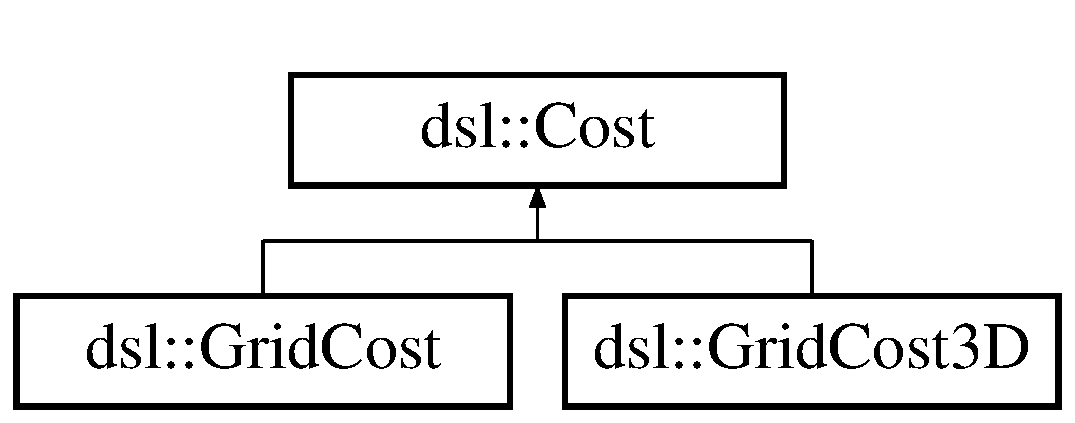
\includegraphics[height=2.000000cm]{classdsl_1_1Cost}
\end{center}
\end{figure}
\subsection*{\-Public \-Member \-Functions}
\begin{DoxyCompactItemize}
\item 
virtual double {\bf \-Heur} (const {\bf \-Vertex} \&va, const {\bf \-Vertex} \&vb) const =0
\item 
virtual double {\bf \-Real} (const {\bf \-Vertex} \&va, const {\bf \-Vertex} \&vb) const 
\end{DoxyCompactItemize}


\subsection{\-Detailed \-Description}
\-Interface defining the cost b/n two vertices. \doxyref{\-Graph}{p.}{classdsl_1_1Graph} search algorithms often require two types of cost\-:

$\ast$ the best possible real cost that a path b/n two vertices can have

$\ast$ a heuristic cost that is an underestimate of that real cost but is useful during path searching.

\-This interface defines the two types of costs. \-The heuristic function is more important and subclasses of this interface are required to provide it. \-The real function is used only for tie-\/breaking and is not crucial but could change performance in certain cases.

\-Author\-: \-Marin \-Kobilarov -\/-\/ \-Copyright (\-C) 2004 

\subsection{\-Member \-Function \-Documentation}
\index{dsl\-::\-Cost@{dsl\-::\-Cost}!\-Heur@{\-Heur}}
\index{\-Heur@{\-Heur}!dsl::Cost@{dsl\-::\-Cost}}
\subsubsection[{\-Heur}]{\setlength{\rightskip}{0pt plus 5cm}virtual double {\bf dsl\-::\-Cost\-::\-Heur} (
\begin{DoxyParamCaption}
\item[{const {\bf \-Vertex} \&}]{va, }
\item[{const {\bf \-Vertex} \&}]{vb}
\end{DoxyParamCaption}
) const\hspace{0.3cm}{\ttfamily  [pure virtual]}}\label{classdsl_1_1Cost_a585a274e68a75de0c9ede55864d6e845}
\-Heuristic distance (should be admissible, i.\-e. less than the real minimum distance) b/n two vertices. \-Subclasses must provide this function 
\begin{DoxyParams}{\-Parameters}
{\em va} & first vertex \\
\hline
{\em vb} & second vertex \\
\hline
\end{DoxyParams}
\begin{DoxyReturn}{\-Returns}
heuristic distance (optimal cost) 
\end{DoxyReturn}


\-Implemented in {\bf dsl\-::\-Grid\-Cost} \doxyref{}{p.}{classdsl_1_1GridCost_a5bb94399b682367c5134a8780adf6598}, and {\bf dsl\-::\-Grid\-Cost3\-D} \doxyref{}{p.}{classdsl_1_1GridCost3D_a3bb22c4a85612a3dfa47d443fb75efff}.



\-Referenced by dsl\-::\-Search\-::\-Calculate\-Ext\-Key(), dsl\-::\-Search\-::\-Plan(), \-Real(), and dsl\-::\-Search\-::\-Set\-Goal().

\index{dsl\-::\-Cost@{dsl\-::\-Cost}!\-Real@{\-Real}}
\index{\-Real@{\-Real}!dsl::Cost@{dsl\-::\-Cost}}
\subsubsection[{\-Real}]{\setlength{\rightskip}{0pt plus 5cm}double {\bf \-Cost\-::\-Real} (
\begin{DoxyParamCaption}
\item[{const {\bf \-Vertex} \&}]{va, }
\item[{const {\bf \-Vertex} \&}]{vb}
\end{DoxyParamCaption}
) const\hspace{0.3cm}{\ttfamily  [virtual]}}\label{classdsl_1_1Cost_a92a686af3e0d416d6f3b03eb1fa1c570}
\-Real best possible distance b/n two vertices. \-Subclasses should optionally provide this function. \-By default it is the heuristic function + epsilon 
\begin{DoxyParams}{\-Parameters}
{\em va} & first vertex \\
\hline
{\em vb} & second vertex \\
\hline
\end{DoxyParams}
\begin{DoxyReturn}{\-Returns}
real minimum possible cost b/n va and vb 
\end{DoxyReturn}


\-Reimplemented in {\bf dsl\-::\-Grid\-Cost} \doxyref{}{p.}{classdsl_1_1GridCost_aeca4afaa0d40c6489791fed0b26c2b55}, and {\bf dsl\-::\-Grid\-Cost3\-D} \doxyref{}{p.}{classdsl_1_1GridCost3D_a6c5ee4a7157f48061284bdcf9deb2b2b}.



\-References \-Heur().



\-Referenced by dsl\-::\-Search\-::\-Min\-Succ().



\-The documentation for this class was generated from the following files\-:\begin{DoxyCompactItemize}
\item 
/home/matt/dsl/lib/{\bf cost.\-h}\item 
/home/matt/dsl/lib/{\bf cost.\-cc}\end{DoxyCompactItemize}

\section{dsl\-:\-:\-Dist\-Edge\-Cost \-Class \-Reference}
\label{classdsl_1_1DistEdgeCost}\index{dsl\-::\-Dist\-Edge\-Cost@{dsl\-::\-Dist\-Edge\-Cost}}


{\ttfamily \#include $<$distedgecost.\-h$>$}

\-Inheritance diagram for dsl\-:\-:\-Dist\-Edge\-Cost\-:\begin{figure}[H]
\begin{center}
\leavevmode
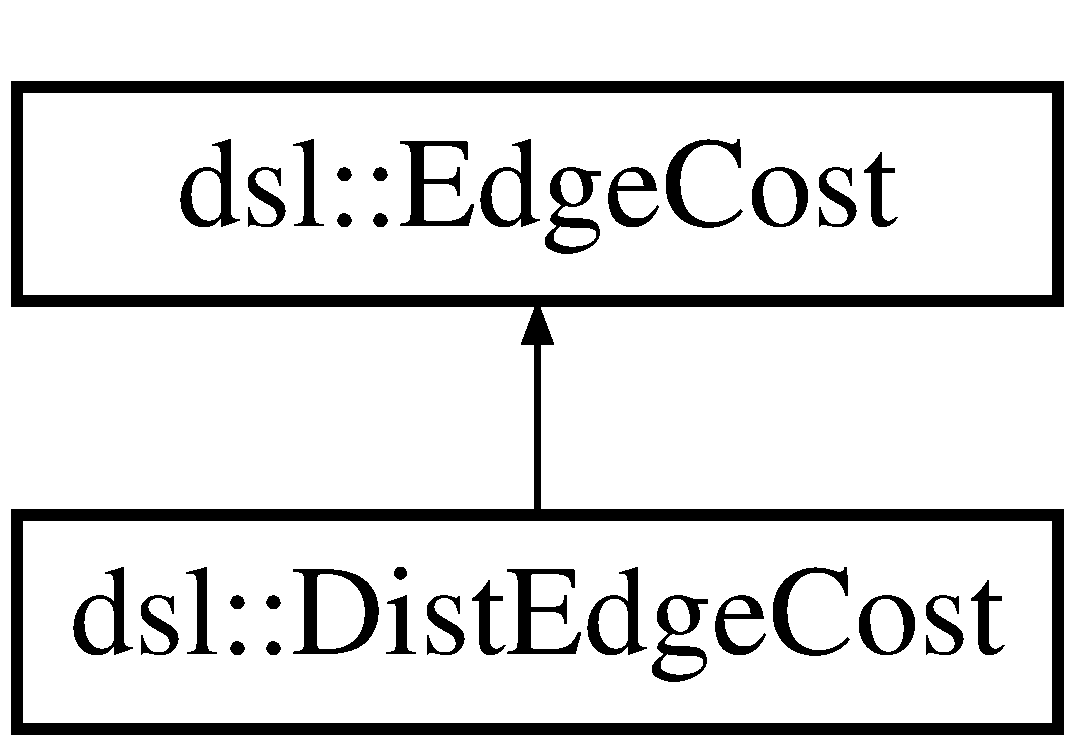
\includegraphics[height=2.000000cm]{classdsl_1_1DistEdgeCost}
\end{center}
\end{figure}
\subsection*{\-Public \-Member \-Functions}
\begin{DoxyCompactItemize}
\item 
virtual double {\bf \-Calc\-Edge\-Cost} (double v1cost, double v2cost, double elength)
\end{DoxyCompactItemize}


\subsection{\-Member \-Function \-Documentation}
\index{dsl\-::\-Dist\-Edge\-Cost@{dsl\-::\-Dist\-Edge\-Cost}!\-Calc\-Edge\-Cost@{\-Calc\-Edge\-Cost}}
\index{\-Calc\-Edge\-Cost@{\-Calc\-Edge\-Cost}!dsl::DistEdgeCost@{dsl\-::\-Dist\-Edge\-Cost}}
\subsubsection[{\-Calc\-Edge\-Cost}]{\setlength{\rightskip}{0pt plus 5cm}double {\bf \-Dist\-Edge\-Cost\-::\-Calc\-Edge\-Cost} (
\begin{DoxyParamCaption}
\item[{double}]{v1cost, }
\item[{double}]{v2cost, }
\item[{double}]{elength}
\end{DoxyParamCaption}
)\hspace{0.3cm}{\ttfamily  [virtual]}}\label{classdsl_1_1DistEdgeCost_a8dcea43332bf660ebe083946c0b5d893}
\-Calculates the cost (usually a height) gradient between two vertices. param v1cost cost of \char`\"{}from\char`\"{} vertex param v2cost cost of \char`\"{}to\char`\"{} vertex param ecost cost of edge 

\-Implements {\bf dsl\-::\-Edge\-Cost} \doxyref{}{p.}{classdsl_1_1EdgeCost_ae09d4d844afd0dda495013c4279ced33}.



\-The documentation for this class was generated from the following files\-:\begin{DoxyCompactItemize}
\item 
/home/matt/dsl/lib/{\bf distedgecost.\-h}\item 
/home/matt/dsl/lib/{\bf distedgecost.\-cc}\end{DoxyCompactItemize}

\section{dsl\-:\-:Edge Class Reference}
\label{classdsl_1_1Edge}\index{dsl\-::\-Edge@{dsl\-::\-Edge}}


{\ttfamily \#include $<$edge.\-h$>$}

\subsection*{Public Member Functions}
\begin{DoxyCompactItemize}
\item 
{\bf Edge} ({\bf Vertex} $\ast${\bf from}=0, {\bf Vertex} $\ast${\bf to}=0, double {\bf cost}=0)
\item 
virtual {\bf $\sim$\-Edge} ()
\end{DoxyCompactItemize}
\subsection*{Public Attributes}
\begin{DoxyCompactItemize}
\item 
int {\bf id}
\begin{DoxyCompactList}\small\item\em edge id (set internally) \end{DoxyCompactList}\item 
{\bf Vertex} $\ast$ {\bf from}
\begin{DoxyCompactList}\small\item\em from vertex \end{DoxyCompactList}\item 
{\bf Vertex} $\ast$ {\bf to}
\begin{DoxyCompactList}\small\item\em to vertex \end{DoxyCompactList}\item 
double {\bf cost}
\begin{DoxyCompactList}\small\item\em cost \end{DoxyCompactList}\item 
double {\bf cost\-Change}
\begin{DoxyCompactList}\small\item\em change in cost (used internally) \end{DoxyCompactList}\end{DoxyCompactItemize}
\subsection*{Friends}
\begin{DoxyCompactItemize}
\item 
class {\bf Graph}
\item 
class {\bf Search}
\item 
std\-::ostream \& {\bf operator$<$$<$} (std\-::ostream \&os, const {\bf Edge} \&e)
\item 
std\-::istream \& {\bf operator$>$$>$} (std\-::istream \&is, {\bf Edge} \&e)
\end{DoxyCompactItemize}


\subsection{Detailed Description}
A generic edge b/n two vertices. Contains an edge cost as well as a cost\-Change variable that could be used for path planning/replanning algorithms such as D$\ast$ (see Dsl)

Author\-: Marin Kobilarov -- Copyright (C) 2004 

\subsection{Constructor \& Destructor Documentation}
\index{dsl\-::\-Edge@{dsl\-::\-Edge}!Edge@{Edge}}
\index{Edge@{Edge}!dsl::Edge@{dsl\-::\-Edge}}
\subsubsection[{Edge}]{\setlength{\rightskip}{0pt plus 5cm}Edge\-::\-Edge (
\begin{DoxyParamCaption}
\item[{{\bf Vertex} $\ast$}]{from = {\ttfamily 0}, }
\item[{{\bf Vertex} $\ast$}]{to = {\ttfamily 0}, }
\item[{double}]{cost = {\ttfamily 0}}
\end{DoxyParamCaption}
)}\label{classdsl_1_1Edge_a9aa20eb48ecb9f296665da92aed6291b}
Initialize an edge using two vertices and a cost; all parameters are optional since an edge does not physically need to connect two vertices or have associated cost 
\begin{DoxyParams}{Parameters}
{\em from} & from vertext (optional) \\
\hline
{\em to} & to vertex (optional) \\
\hline
{\em cost} & cost (optional) \\
\hline
\end{DoxyParams}
\index{dsl\-::\-Edge@{dsl\-::\-Edge}!$\sim$\-Edge@{$\sim$\-Edge}}
\index{$\sim$\-Edge@{$\sim$\-Edge}!dsl::Edge@{dsl\-::\-Edge}}
\subsubsection[{$\sim$\-Edge}]{\setlength{\rightskip}{0pt plus 5cm}Edge\-::$\sim$\-Edge (
\begin{DoxyParamCaption}
{}
\end{DoxyParamCaption}
)\hspace{0.3cm}{\ttfamily [virtual]}}\label{classdsl_1_1Edge_a2f37b72f044427961d6730943daf10e0}


\subsection{Friends And Related Function Documentation}
\index{dsl\-::\-Edge@{dsl\-::\-Edge}!Graph@{Graph}}
\index{Graph@{Graph}!dsl::Edge@{dsl\-::\-Edge}}
\subsubsection[{Graph}]{\setlength{\rightskip}{0pt plus 5cm}friend class {\bf Graph}\hspace{0.3cm}{\ttfamily [friend]}}\label{classdsl_1_1Edge_afab89afd724f1b07b1aaad6bdc61c47a}
\index{dsl\-::\-Edge@{dsl\-::\-Edge}!operator$<$$<$@{operator$<$$<$}}
\index{operator$<$$<$@{operator$<$$<$}!dsl::Edge@{dsl\-::\-Edge}}
\subsubsection[{operator$<$$<$}]{\setlength{\rightskip}{0pt plus 5cm}std\-::ostream\& operator$<$$<$ (
\begin{DoxyParamCaption}
\item[{std\-::ostream \&}]{os, }
\item[{const {\bf Edge} \&}]{e}
\end{DoxyParamCaption}
)\hspace{0.3cm}{\ttfamily [friend]}}\label{classdsl_1_1Edge_aa1b374eb64c6c754621b4fc918a9df57}
Output the edge to a stream 
\begin{DoxyParams}{Parameters}
{\em os} & output stream \\
\hline
{\em e} & edge \\
\hline
\end{DoxyParams}
\begin{DoxyReturn}{Returns}
the output stream 
\end{DoxyReturn}
\index{dsl\-::\-Edge@{dsl\-::\-Edge}!operator$>$$>$@{operator$>$$>$}}
\index{operator$>$$>$@{operator$>$$>$}!dsl::Edge@{dsl\-::\-Edge}}
\subsubsection[{operator$>$$>$}]{\setlength{\rightskip}{0pt plus 5cm}std\-::istream\& operator$>$$>$ (
\begin{DoxyParamCaption}
\item[{std\-::istream \&}]{is, }
\item[{{\bf Edge} \&}]{e}
\end{DoxyParamCaption}
)\hspace{0.3cm}{\ttfamily [friend]}}\label{classdsl_1_1Edge_a40e320f0d46c447d7a361225e43abb25}
Input the edge from a stream 
\begin{DoxyParams}{Parameters}
{\em is} & input stream \\
\hline
{\em e} & edge \\
\hline
\end{DoxyParams}
\begin{DoxyReturn}{Returns}
the input stream 
\end{DoxyReturn}
\index{dsl\-::\-Edge@{dsl\-::\-Edge}!Search@{Search}}
\index{Search@{Search}!dsl::Edge@{dsl\-::\-Edge}}
\subsubsection[{Search}]{\setlength{\rightskip}{0pt plus 5cm}friend class {\bf Search}\hspace{0.3cm}{\ttfamily [friend]}}\label{classdsl_1_1Edge_aea88561fddd2e924cebf793f0cfdc8b6}


\subsection{Member Data Documentation}
\index{dsl\-::\-Edge@{dsl\-::\-Edge}!cost@{cost}}
\index{cost@{cost}!dsl::Edge@{dsl\-::\-Edge}}
\subsubsection[{cost}]{\setlength{\rightskip}{0pt plus 5cm}double dsl\-::\-Edge\-::cost}\label{classdsl_1_1Edge_a2118fb06bf1a19ceffa4303caf41fc14}


cost 



Referenced by dsl\-::\-Graph\-::\-Add\-Edge(), dsl\-::\-Search\-::\-Change\-Cost(), dsl\-::\-Search\-::\-Compute\-Shortest\-Path(), dsl\-::\-Search\-::\-Min\-Succ(), dsl\-::operator$<$$<$(), dsl\-::\-Search\-::\-Plan(), and dsl\-::\-Graph\-::\-Remove\-Edge().

\index{dsl\-::\-Edge@{dsl\-::\-Edge}!cost\-Change@{cost\-Change}}
\index{cost\-Change@{cost\-Change}!dsl::Edge@{dsl\-::\-Edge}}
\subsubsection[{cost\-Change}]{\setlength{\rightskip}{0pt plus 5cm}double dsl\-::\-Edge\-::cost\-Change}\label{classdsl_1_1Edge_a509db0804dbae524bc34cf89a53183fb}


change in cost (used internally) 



Referenced by dsl\-::\-Search\-::\-Change\-Cost(), dsl\-::operator$<$$<$(), dsl\-::\-Search\-::\-Plan(), and dsl\-::\-Graph\-::\-Remove\-Edge().

\index{dsl\-::\-Edge@{dsl\-::\-Edge}!from@{from}}
\index{from@{from}!dsl::Edge@{dsl\-::\-Edge}}
\subsubsection[{from}]{\setlength{\rightskip}{0pt plus 5cm}{\bf Vertex}$\ast$ dsl\-::\-Edge\-::from}\label{classdsl_1_1Edge_a90a355b5bf47c67fcb20f795d88ef5e3}


from vertex 



Referenced by dsl\-::\-Graph\-::\-Add\-Edge(), dsl\-::\-Search\-::\-Compute\-Shortest\-Path(), dsl\-::\-Vertex\-::\-Find(), dsl\-::operator$<$$<$(), dsl\-::\-Search\-::\-Plan(), and dsl\-::\-Graph\-::\-Remove\-Edge().

\index{dsl\-::\-Edge@{dsl\-::\-Edge}!id@{id}}
\index{id@{id}!dsl::Edge@{dsl\-::\-Edge}}
\subsubsection[{id}]{\setlength{\rightskip}{0pt plus 5cm}int dsl\-::\-Edge\-::id}\label{classdsl_1_1Edge_a274a19c8792a79675b643098c2524b84}


edge id (set internally) 



Referenced by dsl\-::\-Graph\-::\-Add\-Edge(), dsl\-::operator$<$$<$(), and dsl\-::\-Graph\-::\-Remove\-Edge().

\index{dsl\-::\-Edge@{dsl\-::\-Edge}!to@{to}}
\index{to@{to}!dsl::Edge@{dsl\-::\-Edge}}
\subsubsection[{to}]{\setlength{\rightskip}{0pt plus 5cm}{\bf Vertex}$\ast$ dsl\-::\-Edge\-::to}\label{classdsl_1_1Edge_aa2f851d9d63e51cf54b5d10412ef7735}


to vertex 



Referenced by dsl\-::\-Graph\-::\-Add\-Edge(), dsl\-::\-Vertex\-::\-Find(), dsl\-::\-Search\-::\-Min\-Succ(), dsl\-::operator$<$$<$(), dsl\-::\-Search\-::\-Plan(), and dsl\-::\-Graph\-::\-Remove\-Edge().



The documentation for this class was generated from the following files\-:\begin{DoxyCompactItemize}
\item 
lib/{\bf edge.\-h}\item 
lib/{\bf edge.\-cc}\end{DoxyCompactItemize}

\section{dsl\-:\-:\-Edge\-Cost \-Class \-Reference}
\label{classdsl_1_1EdgeCost}\index{dsl\-::\-Edge\-Cost@{dsl\-::\-Edge\-Cost}}


{\ttfamily \#include $<$edgecost.\-h$>$}

\-Inheritance diagram for dsl\-:\-:\-Edge\-Cost\-:\begin{figure}[H]
\begin{center}
\leavevmode
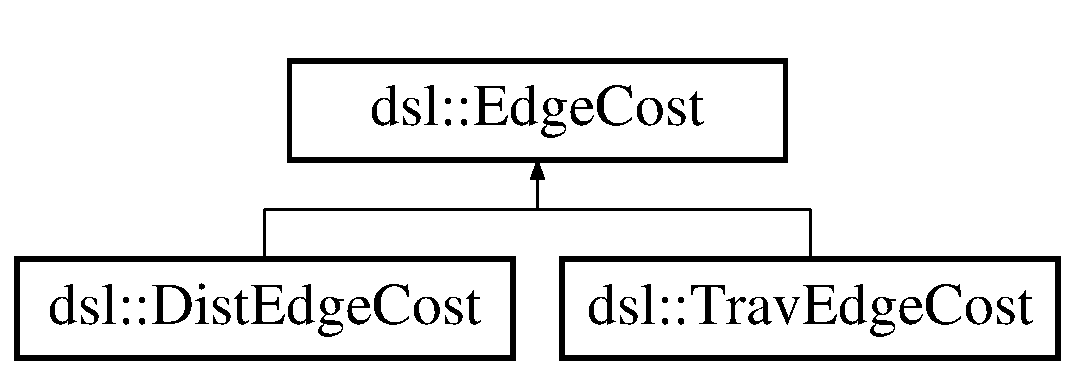
\includegraphics[height=2.000000cm]{classdsl_1_1EdgeCost}
\end{center}
\end{figure}
\subsection*{\-Public \-Member \-Functions}
\begin{DoxyCompactItemize}
\item 
virtual double {\bf \-Calc\-Edge\-Cost} (double v1cost, double v2cost, double elength)=0
\end{DoxyCompactItemize}


\subsection{\-Member \-Function \-Documentation}
\index{dsl\-::\-Edge\-Cost@{dsl\-::\-Edge\-Cost}!\-Calc\-Edge\-Cost@{\-Calc\-Edge\-Cost}}
\index{\-Calc\-Edge\-Cost@{\-Calc\-Edge\-Cost}!dsl::EdgeCost@{dsl\-::\-Edge\-Cost}}
\subsubsection[{\-Calc\-Edge\-Cost}]{\setlength{\rightskip}{0pt plus 5cm}virtual double {\bf dsl\-::\-Edge\-Cost\-::\-Calc\-Edge\-Cost} (
\begin{DoxyParamCaption}
\item[{double}]{v1cost, }
\item[{double}]{v2cost, }
\item[{double}]{elength}
\end{DoxyParamCaption}
)\hspace{0.3cm}{\ttfamily  [pure virtual]}}\label{classdsl_1_1EdgeCost_ae09d4d844afd0dda495013c4279ced33}
\-Calculates the cost (usually a height) gradient between two vertices. param v1cost cost of \char`\"{}from\char`\"{} vertex param v2cost cost of \char`\"{}to\char`\"{} vertex param ecost cost of edge 

\-Implemented in {\bf dsl\-::\-Dist\-Edge\-Cost} \doxyref{}{p.}{classdsl_1_1DistEdgeCost_a8dcea43332bf660ebe083946c0b5d893}, and {\bf dsl\-::\-Trav\-Edge\-Cost} \doxyref{}{p.}{classdsl_1_1TravEdgeCost_a76e9ac094eeee2aba70d8cb89b27b2d8}.



\-Referenced by dsl\-::\-Grid\-Search\-::\-Grid\-Search(), and dsl\-::\-Grid\-Search\-::\-Set\-Cost().



\-The documentation for this class was generated from the following file\-:\begin{DoxyCompactItemize}
\item 
/home/matt/dsl/lib/{\bf edgecost.\-h}\end{DoxyCompactItemize}

\section{\-Spline$<$ \-X, \-Y $>$\-:\-:\-Element \-Class \-Reference}
\label{classSpline_1_1Element}\index{\-Spline$<$ X, Y $>$\-::\-Element@{\-Spline$<$ X, Y $>$\-::\-Element}}


{\ttfamily \#include $<$spline.\-h$>$}

\subsection*{\-Public \-Member \-Functions}
\begin{DoxyCompactItemize}
\item 
{\bf \-Element} (\-X \-\_\-x)
\item 
{\bf \-Element} (\-X \-\_\-x, \-Y \-\_\-a, \-Y \-\_\-b, \-Y \-\_\-c, \-Y \-\_\-d)
\item 
\-Y {\bf eval} (const \-X \&xx) const 
\item 
bool {\bf operator$<$} (const {\bf \-Element} \&e) const 
\item 
bool {\bf operator$<$} (const \-X \&xx) const 
\end{DoxyCompactItemize}
\subsection*{\-Public \-Attributes}
\begin{DoxyCompactItemize}
\item 
\-X {\bf x}
\item 
\-Y {\bf a}
\item 
\-Y {\bf b}
\item 
\-Y {\bf c}
\item 
\-Y {\bf d}
\end{DoxyCompactItemize}
\subsubsection*{template$<$typename \-X, typename \-Y$>$ class Spline$<$ X, Y $>$\-::\-Element}



\subsection{\-Constructor \& \-Destructor \-Documentation}
\index{\-Spline\-::\-Element@{\-Spline\-::\-Element}!\-Element@{\-Element}}
\index{\-Element@{\-Element}!Spline::Element@{\-Spline\-::\-Element}}
\subsubsection[{\-Element}]{\setlength{\rightskip}{0pt plus 5cm}template$<$typename \-X, typename \-Y$>$ {\bf \-Spline}$<$ \-X, \-Y $>$\-::{\bf \-Element\-::\-Element} (
\begin{DoxyParamCaption}
\item[{\-X}]{\-\_\-x}
\end{DoxyParamCaption}
)\hspace{0.3cm}{\ttfamily  [inline]}}\label{classSpline_1_1Element_a695c4dd8fdc435c30a6f57af535940ee}
\index{\-Spline\-::\-Element@{\-Spline\-::\-Element}!\-Element@{\-Element}}
\index{\-Element@{\-Element}!Spline::Element@{\-Spline\-::\-Element}}
\subsubsection[{\-Element}]{\setlength{\rightskip}{0pt plus 5cm}template$<$typename \-X, typename \-Y$>$ {\bf \-Spline}$<$ \-X, \-Y $>$\-::{\bf \-Element\-::\-Element} (
\begin{DoxyParamCaption}
\item[{\-X}]{\-\_\-x, }
\item[{\-Y}]{\-\_\-a, }
\item[{\-Y}]{\-\_\-b, }
\item[{\-Y}]{\-\_\-c, }
\item[{\-Y}]{\-\_\-d}
\end{DoxyParamCaption}
)\hspace{0.3cm}{\ttfamily  [inline]}}\label{classSpline_1_1Element_a7e96953dd79b35946450917573853999}


\subsection{\-Member \-Function \-Documentation}
\index{\-Spline\-::\-Element@{\-Spline\-::\-Element}!eval@{eval}}
\index{eval@{eval}!Spline::Element@{\-Spline\-::\-Element}}
\subsubsection[{eval}]{\setlength{\rightskip}{0pt plus 5cm}template$<$typename \-X, typename \-Y$>$ \-Y {\bf \-Spline}$<$ \-X, \-Y $>$\-::{\bf \-Element\-::eval} (
\begin{DoxyParamCaption}
\item[{const \-X \&}]{xx}
\end{DoxyParamCaption}
) const\hspace{0.3cm}{\ttfamily  [inline]}}\label{classSpline_1_1Element_a7311d21fcf5c5ddf6650d50a3068d2d4}


\-References \-Spline$<$ X, Y $>$\-::\-Element\-::a, \-Spline$<$ X, Y $>$\-::\-Element\-::b, \-Spline$<$ X, Y $>$\-::\-Element\-::c, \-Spline$<$ X, Y $>$\-::\-Element\-::d, and \-Spline$<$ X, Y $>$\-::\-Element\-::x.

\index{\-Spline\-::\-Element@{\-Spline\-::\-Element}!operator$<$@{operator$<$}}
\index{operator$<$@{operator$<$}!Spline::Element@{\-Spline\-::\-Element}}
\subsubsection[{operator$<$}]{\setlength{\rightskip}{0pt plus 5cm}template$<$typename \-X, typename \-Y$>$ bool {\bf \-Spline}$<$ \-X, \-Y $>$\-::\-Element\-::operator$<$ (
\begin{DoxyParamCaption}
\item[{const {\bf \-Element} \&}]{e}
\end{DoxyParamCaption}
) const\hspace{0.3cm}{\ttfamily  [inline]}}\label{classSpline_1_1Element_a8852e43590a6a049a8ea1d2d4bf5a815}


\-References \-Spline$<$ X, Y $>$\-::\-Element\-::x.

\index{\-Spline\-::\-Element@{\-Spline\-::\-Element}!operator$<$@{operator$<$}}
\index{operator$<$@{operator$<$}!Spline::Element@{\-Spline\-::\-Element}}
\subsubsection[{operator$<$}]{\setlength{\rightskip}{0pt plus 5cm}template$<$typename \-X, typename \-Y$>$ bool {\bf \-Spline}$<$ \-X, \-Y $>$\-::\-Element\-::operator$<$ (
\begin{DoxyParamCaption}
\item[{const \-X \&}]{xx}
\end{DoxyParamCaption}
) const\hspace{0.3cm}{\ttfamily  [inline]}}\label{classSpline_1_1Element_af6975df6a1a988f2b154758097f334d4}


\-References \-Spline$<$ X, Y $>$\-::\-Element\-::x.



\subsection{\-Member \-Data \-Documentation}
\index{\-Spline\-::\-Element@{\-Spline\-::\-Element}!a@{a}}
\index{a@{a}!Spline::Element@{\-Spline\-::\-Element}}
\subsubsection[{a}]{\setlength{\rightskip}{0pt plus 5cm}template$<$typename \-X, typename \-Y$>$ \-Y {\bf \-Spline}$<$ \-X, \-Y $>$\-::{\bf \-Element\-::a}}\label{classSpline_1_1Element_a592445ec2cd3d32aaebfe290f7d875da}


\-Referenced by \-Spline$<$ X, Y $>$\-::\-Element\-::eval().

\index{\-Spline\-::\-Element@{\-Spline\-::\-Element}!b@{b}}
\index{b@{b}!Spline::Element@{\-Spline\-::\-Element}}
\subsubsection[{b}]{\setlength{\rightskip}{0pt plus 5cm}template$<$typename \-X, typename \-Y$>$ \-Y {\bf \-Spline}$<$ \-X, \-Y $>$\-::{\bf \-Element\-::b}}\label{classSpline_1_1Element_af109f201661f37626a794b1e3a55510a}


\-Referenced by \-Spline$<$ X, Y $>$\-::\-Element\-::eval().

\index{\-Spline\-::\-Element@{\-Spline\-::\-Element}!c@{c}}
\index{c@{c}!Spline::Element@{\-Spline\-::\-Element}}
\subsubsection[{c}]{\setlength{\rightskip}{0pt plus 5cm}template$<$typename \-X, typename \-Y$>$ \-Y {\bf \-Spline}$<$ \-X, \-Y $>$\-::{\bf \-Element\-::c}}\label{classSpline_1_1Element_ac07e9001f265749c4911309db45fd683}


\-Referenced by \-Spline$<$ X, Y $>$\-::\-Element\-::eval().

\index{\-Spline\-::\-Element@{\-Spline\-::\-Element}!d@{d}}
\index{d@{d}!Spline::Element@{\-Spline\-::\-Element}}
\subsubsection[{d}]{\setlength{\rightskip}{0pt plus 5cm}template$<$typename \-X, typename \-Y$>$ \-Y {\bf \-Spline}$<$ \-X, \-Y $>$\-::{\bf \-Element\-::d}}\label{classSpline_1_1Element_aea979df0cc618ad6b04c4aef4d8bcbb0}


\-Referenced by \-Spline$<$ X, Y $>$\-::\-Element\-::eval().

\index{\-Spline\-::\-Element@{\-Spline\-::\-Element}!x@{x}}
\index{x@{x}!Spline::Element@{\-Spline\-::\-Element}}
\subsubsection[{x}]{\setlength{\rightskip}{0pt plus 5cm}template$<$typename \-X, typename \-Y$>$ \-X {\bf \-Spline}$<$ \-X, \-Y $>$\-::{\bf \-Element\-::x}}\label{classSpline_1_1Element_a25cad79ff1314448e9af26e9842d72b8}


\-Referenced by \-Spline$<$ X, Y $>$\-::\-Element\-::eval(), and \-Spline$<$ X, Y $>$\-::\-Element\-::operator$<$().



\-The documentation for this class was generated from the following file\-:\begin{DoxyCompactItemize}
\item 
/home/matt/dsl/lib/{\bf spline.\-h}\end{DoxyCompactItemize}

\section{dsl\-:\-:\-Graph \-Class \-Reference}
\label{classdsl_1_1Graph}\index{dsl\-::\-Graph@{dsl\-::\-Graph}}


{\ttfamily \#include $<$graph.\-h$>$}

\subsection*{\-Public \-Member \-Functions}
\begin{DoxyCompactItemize}
\item 
{\bf \-Graph} ()
\item 
virtual {\bf $\sim$\-Graph} ()
\item 
void {\bf \-Add\-Vertex} ({\bf \-Vertex} \&v)
\item 
void {\bf \-Remove\-Vertex} ({\bf \-Vertex} \&v, bool re=true, bool del=false)
\item 
void {\bf \-Add\-Edge} ({\bf \-Edge} \&e)
\item 
void {\bf \-Remove\-Edge} ({\bf \-Edge} \&e, bool update=true, bool del=false)
\item 
bool {\bf \-Exists} (const {\bf \-Vertex} \&v) const 
\end{DoxyCompactItemize}
\subsection*{\-Public \-Attributes}
\begin{DoxyCompactItemize}
\item 
std\-::map$<$ int, {\bf \-Edge} $\ast$ $>$ {\bf edges}
\begin{DoxyCompactList}\small\item\em all edges \end{DoxyCompactList}\item 
std\-::map$<$ int, {\bf \-Vertex} $\ast$ $>$ {\bf vertices}
\begin{DoxyCompactList}\small\item\em all vertices \end{DoxyCompactList}\end{DoxyCompactItemize}
\subsection*{\-Protected \-Attributes}
\begin{DoxyCompactItemize}
\item 
{\bf \-Search} $\ast$ {\bf search}
\begin{DoxyCompactList}\small\item\em search operating on this graph \end{DoxyCompactList}\end{DoxyCompactItemize}
\subsection*{\-Friends}
\begin{DoxyCompactItemize}
\item 
class {\bf \-Search}
\end{DoxyCompactItemize}


\subsection{\-Detailed \-Description}
\-Generic graph data structure using hashtables for storing vertices and edges for quick add/remove ops

\-Author\-: \-Marin \-Kobilarov -\/-\/ \-Copyright (\-C) 2004 

\subsection{\-Constructor \& \-Destructor \-Documentation}
\index{dsl\-::\-Graph@{dsl\-::\-Graph}!\-Graph@{\-Graph}}
\index{\-Graph@{\-Graph}!dsl::Graph@{dsl\-::\-Graph}}
\subsubsection[{\-Graph}]{\setlength{\rightskip}{0pt plus 5cm}{\bf \-Graph\-::\-Graph} (
\begin{DoxyParamCaption}
{}
\end{DoxyParamCaption}
)}\label{classdsl_1_1Graph_ae4c72b8ac4d693c49800a4c7e273654f}
\-Initialize an empty graph \index{dsl\-::\-Graph@{dsl\-::\-Graph}!$\sim$\-Graph@{$\sim$\-Graph}}
\index{$\sim$\-Graph@{$\sim$\-Graph}!dsl::Graph@{dsl\-::\-Graph}}
\subsubsection[{$\sim$\-Graph}]{\setlength{\rightskip}{0pt plus 5cm}{\bf \-Graph\-::$\sim$\-Graph} (
\begin{DoxyParamCaption}
{}
\end{DoxyParamCaption}
)\hspace{0.3cm}{\ttfamily  [virtual]}}\label{classdsl_1_1Graph_a902c5b3eacb66d60752525ab23297a95}


\subsection{\-Member \-Function \-Documentation}
\index{dsl\-::\-Graph@{dsl\-::\-Graph}!\-Add\-Edge@{\-Add\-Edge}}
\index{\-Add\-Edge@{\-Add\-Edge}!dsl::Graph@{dsl\-::\-Graph}}
\subsubsection[{\-Add\-Edge}]{\setlength{\rightskip}{0pt plus 5cm}void {\bf \-Graph\-::\-Add\-Edge} (
\begin{DoxyParamCaption}
\item[{{\bf \-Edge} \&}]{e}
\end{DoxyParamCaption}
)}\label{classdsl_1_1Graph_aa4c0322501870143cafbe86a0bc0859d}
\-Add edge. \-If the from/to vertices of the edge are set then they are modified to incude this edge in their outgoing/incoming respectively list of edges 
\begin{DoxyParams}{\-Parameters}
{\em e} & edge \\
\hline
\end{DoxyParams}


\-References dsl\-::\-Search\-::\-Change\-Cost(), dsl\-::\-Edge\-::cost, edges, dsl\-::\-Edge\-::from, dsl\-::\-Edge\-::id, dsl\-::\-Vertex\-::in, \-I\-N\-F, dsl\-::\-Search\-::last, dsl\-::\-Vertex\-::out, search, and dsl\-::\-Edge\-::to.



\-Referenced by dsl\-::\-Grid\-Search\-::\-Add\-Edge(), dsl\-::\-Grid\-Search3\-D\-::\-Add\-Edge(), dsl\-::\-Grid\-Search\-::\-Grid\-Search(), dsl\-::\-Grid\-Search3\-D\-::\-Grid\-Search3\-D(), and dsl\-::\-Trav\-Search\-::\-Trav\-Search().

\index{dsl\-::\-Graph@{dsl\-::\-Graph}!\-Add\-Vertex@{\-Add\-Vertex}}
\index{\-Add\-Vertex@{\-Add\-Vertex}!dsl::Graph@{dsl\-::\-Graph}}
\subsubsection[{\-Add\-Vertex}]{\setlength{\rightskip}{0pt plus 5cm}void {\bf \-Graph\-::\-Add\-Vertex} (
\begin{DoxyParamCaption}
\item[{{\bf \-Vertex} \&}]{v}
\end{DoxyParamCaption}
)}\label{classdsl_1_1Graph_a2a76d7d84d7af2151c9c9b3af5a88b68}
\-Add vertex. \doxyref{\-Vertex}{p.}{classdsl_1_1Vertex} is added to map of vertices. \-No other graph elements are modified. 
\begin{DoxyParams}{\-Parameters}
{\em v} & vertex \\
\hline
\end{DoxyParams}


\-References dsl\-::\-Vertex\-::id, and vertices.



\-Referenced by dsl\-::\-Grid\-Search\-::\-Grid\-Search(), and dsl\-::\-Grid\-Search3\-D\-::\-Grid\-Search3\-D().

\index{dsl\-::\-Graph@{dsl\-::\-Graph}!\-Exists@{\-Exists}}
\index{\-Exists@{\-Exists}!dsl::Graph@{dsl\-::\-Graph}}
\subsubsection[{\-Exists}]{\setlength{\rightskip}{0pt plus 5cm}bool {\bf \-Graph\-::\-Exists} (
\begin{DoxyParamCaption}
\item[{const {\bf \-Vertex} \&}]{v}
\end{DoxyParamCaption}
) const}\label{classdsl_1_1Graph_ab951b71f46e614c43ac235c5340652d4}
\-Checks if a vertex exists 
\begin{DoxyParams}{\-Parameters}
{\em v} & the vertex \\
\hline
\end{DoxyParams}
\begin{DoxyReturn}{\-Returns}
true if present in the graph 
\end{DoxyReturn}


\-References dsl\-::\-Vertex\-::id, and vertices.

\index{dsl\-::\-Graph@{dsl\-::\-Graph}!\-Remove\-Edge@{\-Remove\-Edge}}
\index{\-Remove\-Edge@{\-Remove\-Edge}!dsl::Graph@{dsl\-::\-Graph}}
\subsubsection[{\-Remove\-Edge}]{\setlength{\rightskip}{0pt plus 5cm}void {\bf \-Graph\-::\-Remove\-Edge} (
\begin{DoxyParamCaption}
\item[{{\bf \-Edge} \&}]{e, }
\item[{bool}]{update = {\ttfamily true}, }
\item[{bool}]{del = {\ttfamily false}}
\end{DoxyParamCaption}
)}\label{classdsl_1_1Graph_afb56c9c3db9c8eb30c004ce26373003f}
\-Remove edge. \-If the from/to vertices of the edge are set then they are modified to remove this edge in their outgoing/incoming respectively list of edges 
\begin{DoxyParams}{\-Parameters}
{\em e} & edge \\
\hline
{\em update} & whether to update the graph/search data to reflect the influence of removing this edge if this is done during search. \-Normally, one can pass update=false only when cleaning up the graph upon deletion, for efficiency \\
\hline
{\em del} & delete/free all removed data? (false by default, the idea is that we care more about speed rather than memory; and these will be deleted when the graph object is deleted anyways) \\
\hline
\end{DoxyParams}


\-References dsl\-::\-Edge\-::cost, dsl\-::\-Edge\-::cost\-Change, edges, dsl\-::\-Search\-::\-Eq(), dsl\-::\-Edge\-::from, dsl\-::\-Vertex\-::g, dsl\-::\-Search\-::goal, dsl\-::\-Edge\-::id, dsl\-::\-Vertex\-::in, \-I\-N\-F, dsl\-::\-Search\-::last, dsl\-::\-Search\-::\-Min\-Succ(), dsl\-::\-Vertex\-::open\-List\-Node, dsl\-::\-Vertex\-::out, dsl\-::\-Vertex\-::rhs, search, dsl\-::\-Edge\-::to, and dsl\-::\-Search\-::\-Update\-Vertex().



\-Referenced by \-Remove\-Vertex().

\index{dsl\-::\-Graph@{dsl\-::\-Graph}!\-Remove\-Vertex@{\-Remove\-Vertex}}
\index{\-Remove\-Vertex@{\-Remove\-Vertex}!dsl::Graph@{dsl\-::\-Graph}}
\subsubsection[{\-Remove\-Vertex}]{\setlength{\rightskip}{0pt plus 5cm}void {\bf \-Graph\-::\-Remove\-Vertex} (
\begin{DoxyParamCaption}
\item[{{\bf \-Vertex} \&}]{v, }
\item[{bool}]{re = {\ttfamily true}, }
\item[{bool}]{del = {\ttfamily false}}
\end{DoxyParamCaption}
)}\label{classdsl_1_1Graph_a3f1e66ac1512a70794d90e99edd2a0f9}
\-Remove vertex v. \-Incoming and outgoing edges are removed by default but can be kept intact if paramter re is set ot false 
\begin{DoxyParams}{\-Parameters}
{\em v} & vertex \\
\hline
{\em re} & remove edges? (true by default) \\
\hline
{\em del} & delete/free all removed data? (false by default) \\
\hline
\end{DoxyParams}


\-References dsl\-::\-Vertex\-::id, dsl\-::\-Vertex\-::in, dsl\-::\-Search\-::last, dsl\-::\-Vertex\-::out, dsl\-::\-Search\-::\-Remove(), \-Remove\-Edge(), search, and vertices.



\-Referenced by dsl\-::\-Grid\-Search\-::\-Remove\-Vertex(), and dsl\-::\-Grid\-Search3\-D\-::\-Remove\-Vertex().



\subsection{\-Friends \-And \-Related \-Function \-Documentation}
\index{dsl\-::\-Graph@{dsl\-::\-Graph}!\-Search@{\-Search}}
\index{\-Search@{\-Search}!dsl::Graph@{dsl\-::\-Graph}}
\subsubsection[{\-Search}]{\setlength{\rightskip}{0pt plus 5cm}friend class {\bf \-Search}\hspace{0.3cm}{\ttfamily  [friend]}}\label{classdsl_1_1Graph_aea88561fddd2e924cebf793f0cfdc8b6}


\subsection{\-Member \-Data \-Documentation}
\index{dsl\-::\-Graph@{dsl\-::\-Graph}!edges@{edges}}
\index{edges@{edges}!dsl::Graph@{dsl\-::\-Graph}}
\subsubsection[{edges}]{\setlength{\rightskip}{0pt plus 5cm}std\-::map$<$int, {\bf \-Edge}$\ast$$>$ {\bf dsl\-::\-Graph\-::edges}}\label{classdsl_1_1Graph_a4469eb2ded476a18414e6d3da30ce25b}


all edges 



\-Referenced by \-Add\-Edge(), and \-Remove\-Edge().

\index{dsl\-::\-Graph@{dsl\-::\-Graph}!search@{search}}
\index{search@{search}!dsl::Graph@{dsl\-::\-Graph}}
\subsubsection[{search}]{\setlength{\rightskip}{0pt plus 5cm}{\bf \-Search}$\ast$ {\bf dsl\-::\-Graph\-::search}\hspace{0.3cm}{\ttfamily  [protected]}}\label{classdsl_1_1Graph_a6e76d9d58448b15cbc96e44cc026a6b3}


search operating on this graph 



\-Referenced by \-Add\-Edge(), dsl\-::\-Search\-::\-Compute\-Shortest\-Path(), \-Remove\-Edge(), and \-Remove\-Vertex().

\index{dsl\-::\-Graph@{dsl\-::\-Graph}!vertices@{vertices}}
\index{vertices@{vertices}!dsl::Graph@{dsl\-::\-Graph}}
\subsubsection[{vertices}]{\setlength{\rightskip}{0pt plus 5cm}std\-::map$<$int, {\bf \-Vertex}$\ast$$>$ {\bf dsl\-::\-Graph\-::vertices}}\label{classdsl_1_1Graph_ad1ed99a9711757a661131e7074fdd32b}


all vertices 



\-Referenced by \-Add\-Vertex(), \-Exists(), \-Remove\-Vertex(), and dsl\-::\-Search\-::\-Reset().



\-The documentation for this class was generated from the following files\-:\begin{DoxyCompactItemize}
\item 
/home/matt/dsl/lib/{\bf graph.\-h}\item 
/home/matt/dsl/lib/{\bf graph.\-cc}\end{DoxyCompactItemize}

\section{dsl\-:\-:Grid\-Cost Class Reference}
\label{classdsl_1_1GridCost}\index{dsl\-::\-Grid\-Cost@{dsl\-::\-Grid\-Cost}}


{\ttfamily \#include $<$gridcost.\-h$>$}

Inheritance diagram for dsl\-:\-:Grid\-Cost\-:\begin{figure}[H]
\begin{center}
\leavevmode
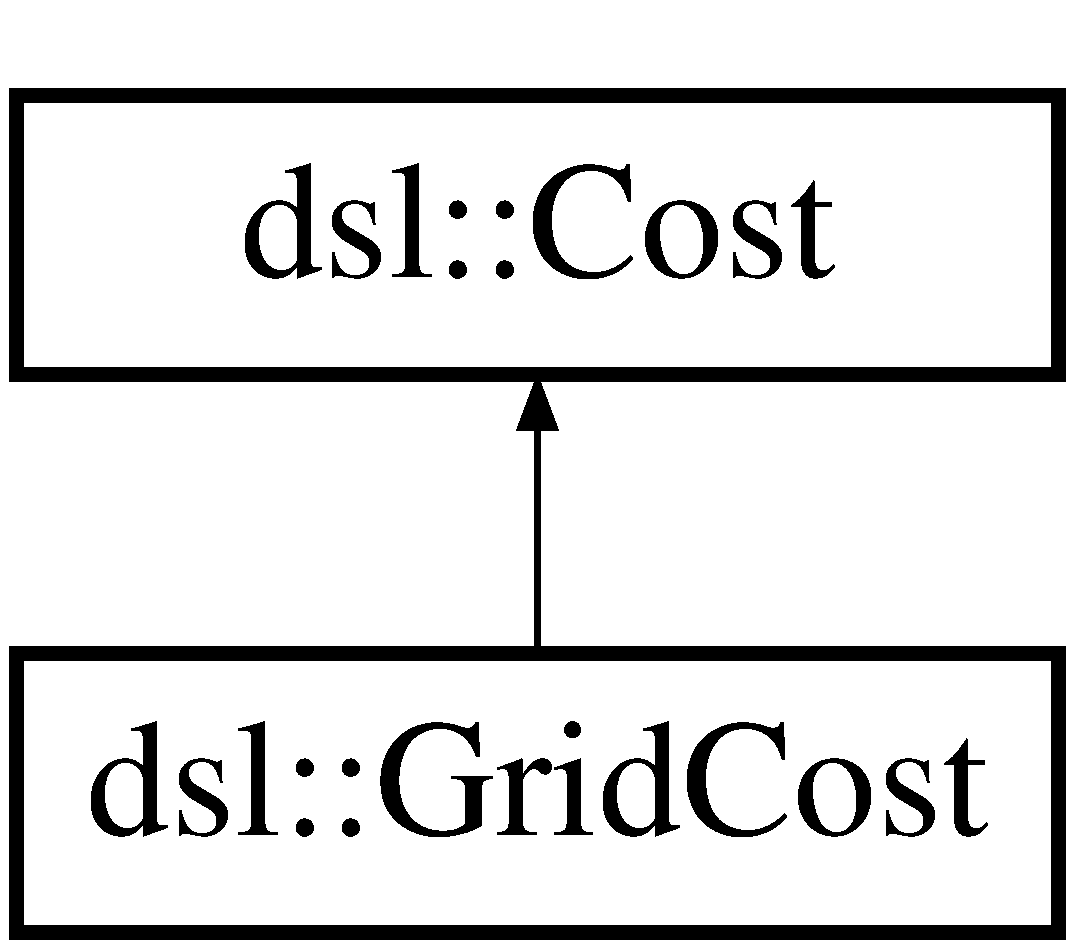
\includegraphics[height=2.000000cm]{classdsl_1_1GridCost}
\end{center}
\end{figure}
\subsection*{Public Member Functions}
\begin{DoxyCompactItemize}
\item 
double {\bf Heur} (const {\bf Vertex} \&va, const {\bf Vertex} \&vb) const 
\item 
double {\bf Real} (const {\bf Vertex} \&va, const {\bf Vertex} \&vb) const 
\end{DoxyCompactItemize}


\subsection{Detailed Description}
Grid cost interface.

Author\-: Marin Kobilarov -- Copyright (C) 2004 

\subsection{Member Function Documentation}
\index{dsl\-::\-Grid\-Cost@{dsl\-::\-Grid\-Cost}!Heur@{Heur}}
\index{Heur@{Heur}!dsl::GridCost@{dsl\-::\-Grid\-Cost}}
\subsubsection[{Heur}]{\setlength{\rightskip}{0pt plus 5cm}double Grid\-Cost\-::\-Heur (
\begin{DoxyParamCaption}
\item[{const {\bf Vertex} \&}]{va, }
\item[{const {\bf Vertex} \&}]{vb}
\end{DoxyParamCaption}
) const\hspace{0.3cm}{\ttfamily [virtual]}}\label{classdsl_1_1GridCost_a5bb94399b682367c5134a8780adf6598}
Heuristic distance (should be admissible, i.\-e. less than the real minimum distance) b/n two vertices. Subclasses must provide this function 
\begin{DoxyParams}{Parameters}
{\em va} & first vertex \\
\hline
{\em vb} & second vertex \\
\hline
\end{DoxyParams}
\begin{DoxyReturn}{Returns}
heuristic distance (optimal cost) 
\end{DoxyReturn}


Implements {\bf dsl\-::\-Cost} \doxyref{}{p.}{classdsl_1_1Cost_a585a274e68a75de0c9ede55864d6e845}.



References dsl\-::\-Vertex\-::data.

\index{dsl\-::\-Grid\-Cost@{dsl\-::\-Grid\-Cost}!Real@{Real}}
\index{Real@{Real}!dsl::GridCost@{dsl\-::\-Grid\-Cost}}
\subsubsection[{Real}]{\setlength{\rightskip}{0pt plus 5cm}double Grid\-Cost\-::\-Real (
\begin{DoxyParamCaption}
\item[{const {\bf Vertex} \&}]{va, }
\item[{const {\bf Vertex} \&}]{vb}
\end{DoxyParamCaption}
) const\hspace{0.3cm}{\ttfamily [virtual]}}\label{classdsl_1_1GridCost_aeca4afaa0d40c6489791fed0b26c2b55}
Real best possible distance b/n two vertices. Subclasses should optionally provide this function. By default it is the heuristic function + epsilon 
\begin{DoxyParams}{Parameters}
{\em va} & first vertex \\
\hline
{\em vb} & second vertex \\
\hline
\end{DoxyParams}
\begin{DoxyReturn}{Returns}
real minimum possible cost b/n va and vb 
\end{DoxyReturn}


Reimplemented from {\bf dsl\-::\-Cost} \doxyref{}{p.}{classdsl_1_1Cost_a92a686af3e0d416d6f3b03eb1fa1c570}.



References dsl\-::\-Vertex\-::data.



The documentation for this class was generated from the following files\-:\begin{DoxyCompactItemize}
\item 
lib/{\bf gridcost.\-h}\item 
lib/{\bf gridcost.\-cc}\end{DoxyCompactItemize}

\section{dsl\-:\-:\-Grid\-Cost3\-D \-Class \-Reference}
\label{classdsl_1_1GridCost3D}\index{dsl\-::\-Grid\-Cost3\-D@{dsl\-::\-Grid\-Cost3\-D}}


{\ttfamily \#include $<$gridcost3d.\-h$>$}

\-Inheritance diagram for dsl\-:\-:\-Grid\-Cost3\-D\-:\begin{figure}[H]
\begin{center}
\leavevmode
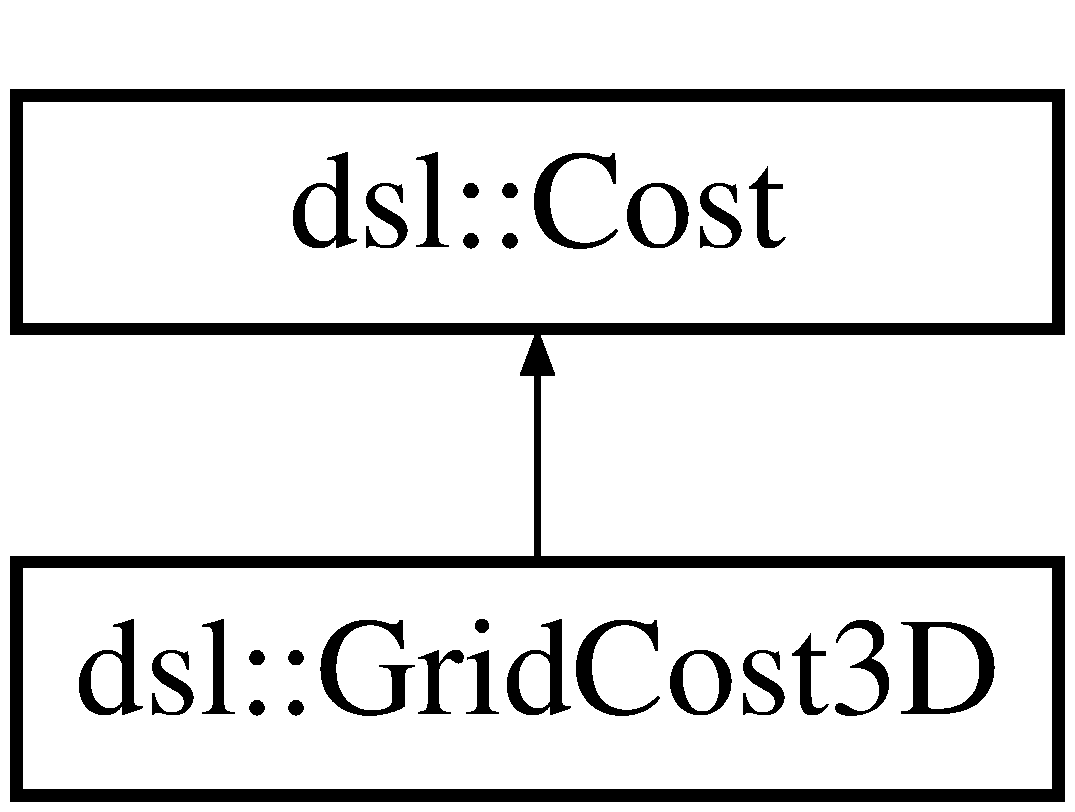
\includegraphics[height=2.000000cm]{classdsl_1_1GridCost3D}
\end{center}
\end{figure}
\subsection*{\-Public \-Member \-Functions}
\begin{DoxyCompactItemize}
\item 
double {\bf \-Heur} (const {\bf \-Vertex} \&va, const {\bf \-Vertex} \&vb) const 
\item 
double {\bf \-Real} (const {\bf \-Vertex} \&va, const {\bf \-Vertex} \&vb) const 
\end{DoxyCompactItemize}


\subsection{\-Detailed \-Description}
3\-D \-Grid cost interface.

\-Author\-: \-Marin \-Kobilarov -\/-\/ \-Copyright (\-C) 2004 

\subsection{\-Member \-Function \-Documentation}
\index{dsl\-::\-Grid\-Cost3\-D@{dsl\-::\-Grid\-Cost3\-D}!\-Heur@{\-Heur}}
\index{\-Heur@{\-Heur}!dsl::GridCost3D@{dsl\-::\-Grid\-Cost3\-D}}
\subsubsection[{\-Heur}]{\setlength{\rightskip}{0pt plus 5cm}double {\bf \-Grid\-Cost3\-D\-::\-Heur} (
\begin{DoxyParamCaption}
\item[{const {\bf \-Vertex} \&}]{va, }
\item[{const {\bf \-Vertex} \&}]{vb}
\end{DoxyParamCaption}
) const\hspace{0.3cm}{\ttfamily  [virtual]}}\label{classdsl_1_1GridCost3D_a3bb22c4a85612a3dfa47d443fb75efff}
\-Heuristic distance (should be admissible, i.\-e. less than the real minimum distance) b/n two vertices. \-Subclasses must provide this function 
\begin{DoxyParams}{\-Parameters}
{\em va} & first vertex \\
\hline
{\em vb} & second vertex \\
\hline
\end{DoxyParams}
\begin{DoxyReturn}{\-Returns}
heuristic distance (optimal cost) 
\end{DoxyReturn}


\-Implements {\bf dsl\-::\-Cost} \doxyref{}{p.}{classdsl_1_1Cost_a585a274e68a75de0c9ede55864d6e845}.



\-References dsl\-::\-Vertex\-::data, and \-M\-A\-X.

\index{dsl\-::\-Grid\-Cost3\-D@{dsl\-::\-Grid\-Cost3\-D}!\-Real@{\-Real}}
\index{\-Real@{\-Real}!dsl::GridCost3D@{dsl\-::\-Grid\-Cost3\-D}}
\subsubsection[{\-Real}]{\setlength{\rightskip}{0pt plus 5cm}double {\bf \-Grid\-Cost3\-D\-::\-Real} (
\begin{DoxyParamCaption}
\item[{const {\bf \-Vertex} \&}]{va, }
\item[{const {\bf \-Vertex} \&}]{vb}
\end{DoxyParamCaption}
) const\hspace{0.3cm}{\ttfamily  [virtual]}}\label{classdsl_1_1GridCost3D_a6c5ee4a7157f48061284bdcf9deb2b2b}
\-Real best possible distance b/n two vertices. \-Subclasses should optionally provide this function. \-By default it is the heuristic function + epsilon 
\begin{DoxyParams}{\-Parameters}
{\em va} & first vertex \\
\hline
{\em vb} & second vertex \\
\hline
\end{DoxyParams}
\begin{DoxyReturn}{\-Returns}
real minimum possible cost b/n va and vb 
\end{DoxyReturn}


\-Reimplemented from {\bf dsl\-::\-Cost} \doxyref{}{p.}{classdsl_1_1Cost_a92a686af3e0d416d6f3b03eb1fa1c570}.



\-References dsl\-::\-Vertex\-::data.



\-The documentation for this class was generated from the following files\-:\begin{DoxyCompactItemize}
\item 
/home/matt/dsl/lib/{\bf gridcost3d.\-h}\item 
/home/matt/dsl/lib/{\bf gridcost3d.\-cc}\end{DoxyCompactItemize}

\section{dsl\-:\-:Grid\-Path Class Reference}
\label{classdsl_1_1GridPath}\index{dsl\-::\-Grid\-Path@{dsl\-::\-Grid\-Path}}


{\ttfamily \#include $<$gridsearch.\-h$>$}

\subsection*{Public Member Functions}
\begin{DoxyCompactItemize}
\item 
{\bf Grid\-Path} ()
\end{DoxyCompactItemize}
\subsection*{Public Attributes}
\begin{DoxyCompactItemize}
\item 
int $\ast$ {\bf pos}
\begin{DoxyCompactList}\small\item\em (x,y) point position array of size 2$\ast$count \end{DoxyCompactList}\item 
int {\bf count}
\begin{DoxyCompactList}\small\item\em number of points along the path \end{DoxyCompactList}\item 
double {\bf len}
\begin{DoxyCompactList}\small\item\em length of path (sum of eucl. distances b/n points) \end{DoxyCompactList}\end{DoxyCompactItemize}


\subsection{Detailed Description}
Path containing a list of grid points 

\subsection{Constructor \& Destructor Documentation}
\index{dsl\-::\-Grid\-Path@{dsl\-::\-Grid\-Path}!Grid\-Path@{Grid\-Path}}
\index{Grid\-Path@{Grid\-Path}!dsl::GridPath@{dsl\-::\-Grid\-Path}}
\subsubsection[{Grid\-Path}]{\setlength{\rightskip}{0pt plus 5cm}dsl\-::\-Grid\-Path\-::\-Grid\-Path (
\begin{DoxyParamCaption}
{}
\end{DoxyParamCaption}
)\hspace{0.3cm}{\ttfamily [inline]}}\label{classdsl_1_1GridPath_accdb54882a5c3f209d016e7386df8ac7}


\subsection{Member Data Documentation}
\index{dsl\-::\-Grid\-Path@{dsl\-::\-Grid\-Path}!count@{count}}
\index{count@{count}!dsl::GridPath@{dsl\-::\-Grid\-Path}}
\subsubsection[{count}]{\setlength{\rightskip}{0pt plus 5cm}int dsl\-::\-Grid\-Path\-::count}\label{classdsl_1_1GridPath_a924ff509ec4ed61c1b1263fbeaecfafa}


number of points along the path 



Referenced by main(), dsl\-::\-Grid\-Search\-::\-Opt\-Path(), and dsl\-::\-Grid\-Search\-::\-Plan().

\index{dsl\-::\-Grid\-Path@{dsl\-::\-Grid\-Path}!len@{len}}
\index{len@{len}!dsl::GridPath@{dsl\-::\-Grid\-Path}}
\subsubsection[{len}]{\setlength{\rightskip}{0pt plus 5cm}double dsl\-::\-Grid\-Path\-::len}\label{classdsl_1_1GridPath_ab9938a9e53a91ac6b01387beadea1535}


length of path (sum of eucl. distances b/n points) 



Referenced by main(), dsl\-::\-Grid\-Search\-::\-Opt\-Path(), and dsl\-::\-Grid\-Search\-::\-Plan().

\index{dsl\-::\-Grid\-Path@{dsl\-::\-Grid\-Path}!pos@{pos}}
\index{pos@{pos}!dsl::GridPath@{dsl\-::\-Grid\-Path}}
\subsubsection[{pos}]{\setlength{\rightskip}{0pt plus 5cm}int$\ast$ dsl\-::\-Grid\-Path\-::pos}\label{classdsl_1_1GridPath_ae631ccfa01d408c5b8ec488c837a397e}


(x,y) point position array of size 2$\ast$count 



Referenced by main(), dsl\-::\-Grid\-Search\-::\-Opt\-Path(), and dsl\-::\-Grid\-Search\-::\-Plan().



The documentation for this class was generated from the following file\-:\begin{DoxyCompactItemize}
\item 
lib/{\bf gridsearch.\-h}\end{DoxyCompactItemize}

\section{dsl\-:\-:\-Grid\-Path3\-D \-Class \-Reference}
\label{classdsl_1_1GridPath3D}\index{dsl\-::\-Grid\-Path3\-D@{dsl\-::\-Grid\-Path3\-D}}


{\ttfamily \#include $<$gridsearch3d.\-h$>$}

\-Inheritance diagram for dsl\-:\-:\-Grid\-Path3\-D\-:\begin{figure}[H]
\begin{center}
\leavevmode
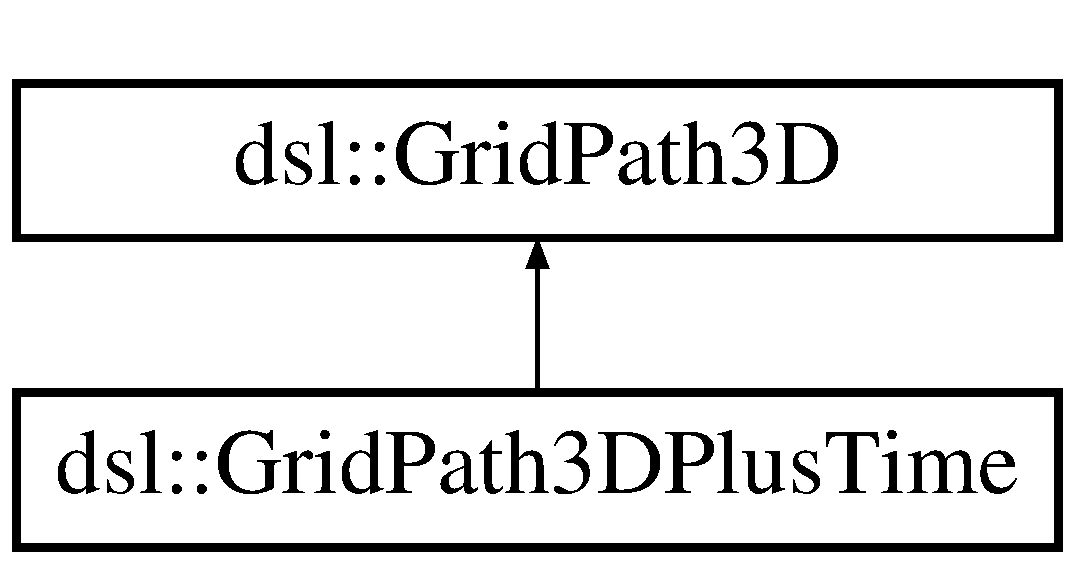
\includegraphics[height=2.000000cm]{classdsl_1_1GridPath3D}
\end{center}
\end{figure}
\subsection*{\-Public \-Member \-Functions}
\begin{DoxyCompactItemize}
\item 
{\bf \-Grid\-Path3\-D} ()
\item 
{\bf \-Grid\-Path3\-D} (const {\bf \-Grid\-Path3\-D} \&)
\item 
virtual {\bf $\sim$\-Grid\-Path3\-D} ()
\item 
void {\bf \-Append\-Path} ({\bf \-Grid\-Path3\-D} \&p)
\end{DoxyCompactItemize}
\subsection*{\-Public \-Attributes}
\begin{DoxyCompactItemize}
\item 
double $\ast$ {\bf pos}
\begin{DoxyCompactList}\small\item\em (x,y,z) point position array of size 3$\ast$count \end{DoxyCompactList}\item 
int {\bf count}
\begin{DoxyCompactList}\small\item\em number of points along the path \end{DoxyCompactList}\item 
double {\bf len}
\begin{DoxyCompactList}\small\item\em length of path (sum of eucl. distances b/n points) \end{DoxyCompactList}\end{DoxyCompactItemize}


\subsection{\-Detailed \-Description}
\-Path containing a list of grid points 

\subsection{\-Constructor \& \-Destructor \-Documentation}
\index{dsl\-::\-Grid\-Path3\-D@{dsl\-::\-Grid\-Path3\-D}!\-Grid\-Path3\-D@{\-Grid\-Path3\-D}}
\index{\-Grid\-Path3\-D@{\-Grid\-Path3\-D}!dsl::GridPath3D@{dsl\-::\-Grid\-Path3\-D}}
\subsubsection[{\-Grid\-Path3\-D}]{\setlength{\rightskip}{0pt plus 5cm}{\bf \-Grid\-Path3\-D\-::\-Grid\-Path3\-D} (
\begin{DoxyParamCaption}
{}
\end{DoxyParamCaption}
)}\label{classdsl_1_1GridPath3D_a291e4292def2e8dd0dbf7cdf138d29e2}
\index{dsl\-::\-Grid\-Path3\-D@{dsl\-::\-Grid\-Path3\-D}!\-Grid\-Path3\-D@{\-Grid\-Path3\-D}}
\index{\-Grid\-Path3\-D@{\-Grid\-Path3\-D}!dsl::GridPath3D@{dsl\-::\-Grid\-Path3\-D}}
\subsubsection[{\-Grid\-Path3\-D}]{\setlength{\rightskip}{0pt plus 5cm}{\bf \-Grid\-Path3\-D\-::\-Grid\-Path3\-D} (
\begin{DoxyParamCaption}
\item[{const {\bf \-Grid\-Path3\-D} \&}]{cp}
\end{DoxyParamCaption}
)}\label{classdsl_1_1GridPath3D_a53eab4ef4b5e6fc10c82de0d0e5a2ced}


\-References count, len, and pos.

\index{dsl\-::\-Grid\-Path3\-D@{dsl\-::\-Grid\-Path3\-D}!$\sim$\-Grid\-Path3\-D@{$\sim$\-Grid\-Path3\-D}}
\index{$\sim$\-Grid\-Path3\-D@{$\sim$\-Grid\-Path3\-D}!dsl::GridPath3D@{dsl\-::\-Grid\-Path3\-D}}
\subsubsection[{$\sim$\-Grid\-Path3\-D}]{\setlength{\rightskip}{0pt plus 5cm}{\bf \-Grid\-Path3\-D\-::$\sim$\-Grid\-Path3\-D} (
\begin{DoxyParamCaption}
{}
\end{DoxyParamCaption}
)\hspace{0.3cm}{\ttfamily  [virtual]}}\label{classdsl_1_1GridPath3D_a396b5e45917fb5cc918c0e84fd9467dc}


\-References pos.



\subsection{\-Member \-Function \-Documentation}
\index{dsl\-::\-Grid\-Path3\-D@{dsl\-::\-Grid\-Path3\-D}!\-Append\-Path@{\-Append\-Path}}
\index{\-Append\-Path@{\-Append\-Path}!dsl::GridPath3D@{dsl\-::\-Grid\-Path3\-D}}
\subsubsection[{\-Append\-Path}]{\setlength{\rightskip}{0pt plus 5cm}void {\bf \-Grid\-Path3\-D\-::\-Append\-Path} (
\begin{DoxyParamCaption}
\item[{{\bf \-Grid\-Path3\-D} \&}]{p}
\end{DoxyParamCaption}
)}\label{classdsl_1_1GridPath3D_a5874eb53228086003984265be3bbbb21}


\-References count, len, and pos.



\subsection{\-Member \-Data \-Documentation}
\index{dsl\-::\-Grid\-Path3\-D@{dsl\-::\-Grid\-Path3\-D}!count@{count}}
\index{count@{count}!dsl::GridPath3D@{dsl\-::\-Grid\-Path3\-D}}
\subsubsection[{count}]{\setlength{\rightskip}{0pt plus 5cm}int {\bf dsl\-::\-Grid\-Path3\-D\-::count}}\label{classdsl_1_1GridPath3D_a350948036dea58011fcc1720e90a5466}


number of points along the path 



\-Referenced by \-Append\-Path(), dsl\-::\-Grid\-Path3\-D\-Plus\-Time\-::\-Append\-Path(), \-Grid\-Path3\-D(), dsl\-::\-Grid\-Path3\-D\-Plus\-Time\-::\-Grid\-Path3\-D\-Plus\-Time(), dsl\-::\-Grid\-Search3\-D\-::\-Opt\-Path(), dsl\-::\-Grid\-Search3\-D\-::\-Plan(), dsl\-::\-Grid\-Search3\-D\-::\-Smooth\-Path\-Bezier(), dsl\-::\-Grid\-Search3\-D\-::\-Smooth\-Path\-Opt\-Cost(), and dsl\-::\-Grid\-Search3\-D\-::\-Smooth\-Path\-Spline().

\index{dsl\-::\-Grid\-Path3\-D@{dsl\-::\-Grid\-Path3\-D}!len@{len}}
\index{len@{len}!dsl::GridPath3D@{dsl\-::\-Grid\-Path3\-D}}
\subsubsection[{len}]{\setlength{\rightskip}{0pt plus 5cm}double {\bf dsl\-::\-Grid\-Path3\-D\-::len}}\label{classdsl_1_1GridPath3D_a9a9295000002fee7806697d075be41d2}


length of path (sum of eucl. distances b/n points) 



\-Referenced by \-Append\-Path(), dsl\-::\-Grid\-Path3\-D\-Plus\-Time\-::\-Append\-Path(), \-Grid\-Path3\-D(), dsl\-::\-Grid\-Search3\-D\-::\-Opt\-Path(), dsl\-::\-Grid\-Search3\-D\-::\-Plan(), dsl\-::\-Grid\-Search3\-D\-::\-Smooth\-Path\-Bezier(), dsl\-::\-Grid\-Search3\-D\-::\-Smooth\-Path\-Opt\-Cost(), and dsl\-::\-Grid\-Search3\-D\-::\-Smooth\-Path\-Spline().

\index{dsl\-::\-Grid\-Path3\-D@{dsl\-::\-Grid\-Path3\-D}!pos@{pos}}
\index{pos@{pos}!dsl::GridPath3D@{dsl\-::\-Grid\-Path3\-D}}
\subsubsection[{pos}]{\setlength{\rightskip}{0pt plus 5cm}double$\ast$ {\bf dsl\-::\-Grid\-Path3\-D\-::pos}}\label{classdsl_1_1GridPath3D_a40d6e7d70427c9233ae8b0e8b2a82124}


(x,y,z) point position array of size 3$\ast$count 



\-Referenced by \-Append\-Path(), \-Grid\-Path3\-D(), dsl\-::\-Grid\-Search3\-D\-::\-Opt\-Path(), dsl\-::\-Grid\-Search3\-D\-::\-Plan(), dsl\-::\-Grid\-Search3\-D\-::\-Smooth\-Path\-Bezier(), dsl\-::\-Grid\-Search3\-D\-::\-Smooth\-Path\-Opt\-Cost(), dsl\-::\-Grid\-Search3\-D\-::\-Smooth\-Path\-Spline(), and $\sim$\-Grid\-Path3\-D().



\-The documentation for this class was generated from the following files\-:\begin{DoxyCompactItemize}
\item 
/home/matt/dsl/lib/{\bf gridsearch3d.\-h}\item 
/home/matt/dsl/lib/{\bf gridsearch3d.\-cc}\end{DoxyCompactItemize}

\section{dsl\-:\-:\-Grid\-Path3\-D\-Plus\-Time \-Class \-Reference}
\label{classdsl_1_1GridPath3DPlusTime}\index{dsl\-::\-Grid\-Path3\-D\-Plus\-Time@{dsl\-::\-Grid\-Path3\-D\-Plus\-Time}}


{\ttfamily \#include $<$gridsearch3d.\-h$>$}

\-Inheritance diagram for dsl\-:\-:\-Grid\-Path3\-D\-Plus\-Time\-:\begin{figure}[H]
\begin{center}
\leavevmode
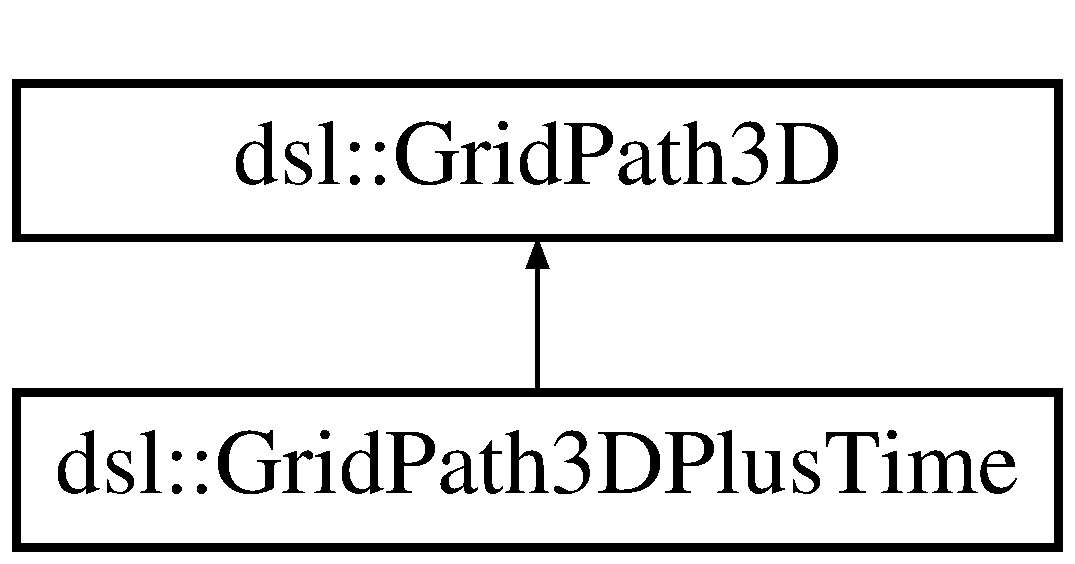
\includegraphics[height=2.000000cm]{classdsl_1_1GridPath3DPlusTime}
\end{center}
\end{figure}
\subsection*{\-Public \-Member \-Functions}
\begin{DoxyCompactItemize}
\item 
{\bf \-Grid\-Path3\-D\-Plus\-Time} ()
\item 
{\bf \-Grid\-Path3\-D\-Plus\-Time} (const {\bf \-Grid\-Path3\-D\-Plus\-Time} \&)
\item 
virtual {\bf $\sim$\-Grid\-Path3\-D\-Plus\-Time} ()
\item 
void {\bf \-Append\-Path} ({\bf \-Grid\-Path3\-D\-Plus\-Time} \&p)
\end{DoxyCompactItemize}
\subsection*{\-Public \-Attributes}
\begin{DoxyCompactItemize}
\item 
double $\ast$ {\bf times}
\end{DoxyCompactItemize}


\subsection{\-Constructor \& \-Destructor \-Documentation}
\index{dsl\-::\-Grid\-Path3\-D\-Plus\-Time@{dsl\-::\-Grid\-Path3\-D\-Plus\-Time}!\-Grid\-Path3\-D\-Plus\-Time@{\-Grid\-Path3\-D\-Plus\-Time}}
\index{\-Grid\-Path3\-D\-Plus\-Time@{\-Grid\-Path3\-D\-Plus\-Time}!dsl::GridPath3DPlusTime@{dsl\-::\-Grid\-Path3\-D\-Plus\-Time}}
\subsubsection[{\-Grid\-Path3\-D\-Plus\-Time}]{\setlength{\rightskip}{0pt plus 5cm}{\bf \-Grid\-Path3\-D\-Plus\-Time\-::\-Grid\-Path3\-D\-Plus\-Time} (
\begin{DoxyParamCaption}
{}
\end{DoxyParamCaption}
)}\label{classdsl_1_1GridPath3DPlusTime_ad19800d4e65b26a57b4e20c6d50f7951}
\index{dsl\-::\-Grid\-Path3\-D\-Plus\-Time@{dsl\-::\-Grid\-Path3\-D\-Plus\-Time}!\-Grid\-Path3\-D\-Plus\-Time@{\-Grid\-Path3\-D\-Plus\-Time}}
\index{\-Grid\-Path3\-D\-Plus\-Time@{\-Grid\-Path3\-D\-Plus\-Time}!dsl::GridPath3DPlusTime@{dsl\-::\-Grid\-Path3\-D\-Plus\-Time}}
\subsubsection[{\-Grid\-Path3\-D\-Plus\-Time}]{\setlength{\rightskip}{0pt plus 5cm}{\bf \-Grid\-Path3\-D\-Plus\-Time\-::\-Grid\-Path3\-D\-Plus\-Time} (
\begin{DoxyParamCaption}
\item[{const {\bf \-Grid\-Path3\-D\-Plus\-Time} \&}]{cp}
\end{DoxyParamCaption}
)}\label{classdsl_1_1GridPath3DPlusTime_af3f459f5b8852a989224aeae989061be}


\-References dsl\-::\-Grid\-Path3\-D\-::count, and times.

\index{dsl\-::\-Grid\-Path3\-D\-Plus\-Time@{dsl\-::\-Grid\-Path3\-D\-Plus\-Time}!$\sim$\-Grid\-Path3\-D\-Plus\-Time@{$\sim$\-Grid\-Path3\-D\-Plus\-Time}}
\index{$\sim$\-Grid\-Path3\-D\-Plus\-Time@{$\sim$\-Grid\-Path3\-D\-Plus\-Time}!dsl::GridPath3DPlusTime@{dsl\-::\-Grid\-Path3\-D\-Plus\-Time}}
\subsubsection[{$\sim$\-Grid\-Path3\-D\-Plus\-Time}]{\setlength{\rightskip}{0pt plus 5cm}{\bf \-Grid\-Path3\-D\-Plus\-Time\-::$\sim$\-Grid\-Path3\-D\-Plus\-Time} (
\begin{DoxyParamCaption}
{}
\end{DoxyParamCaption}
)\hspace{0.3cm}{\ttfamily  [virtual]}}\label{classdsl_1_1GridPath3DPlusTime_a5ff4b9ae19ff17f8e38e94eec331030a}


\-References times.



\subsection{\-Member \-Function \-Documentation}
\index{dsl\-::\-Grid\-Path3\-D\-Plus\-Time@{dsl\-::\-Grid\-Path3\-D\-Plus\-Time}!\-Append\-Path@{\-Append\-Path}}
\index{\-Append\-Path@{\-Append\-Path}!dsl::GridPath3DPlusTime@{dsl\-::\-Grid\-Path3\-D\-Plus\-Time}}
\subsubsection[{\-Append\-Path}]{\setlength{\rightskip}{0pt plus 5cm}void {\bf \-Grid\-Path3\-D\-Plus\-Time\-::\-Append\-Path} (
\begin{DoxyParamCaption}
\item[{{\bf \-Grid\-Path3\-D\-Plus\-Time} \&}]{p}
\end{DoxyParamCaption}
)}\label{classdsl_1_1GridPath3DPlusTime_a97a86495f85c868e9ed0f85d22b38482}


\-References dsl\-::\-Grid\-Path3\-D\-::count, dsl\-::\-Grid\-Path3\-D\-::len, and times.



\subsection{\-Member \-Data \-Documentation}
\index{dsl\-::\-Grid\-Path3\-D\-Plus\-Time@{dsl\-::\-Grid\-Path3\-D\-Plus\-Time}!times@{times}}
\index{times@{times}!dsl::GridPath3DPlusTime@{dsl\-::\-Grid\-Path3\-D\-Plus\-Time}}
\subsubsection[{times}]{\setlength{\rightskip}{0pt plus 5cm}double$\ast$ {\bf dsl\-::\-Grid\-Path3\-D\-Plus\-Time\-::times}}\label{classdsl_1_1GridPath3DPlusTime_a3b68faf25e95e377cc986c2ea40c4ec8}


\-Referenced by \-Append\-Path(), \-Grid\-Path3\-D\-Plus\-Time(), dsl\-::\-Grid\-Search3\-D\-::\-Smooth\-Path\-Opt\-Cost(), dsl\-::\-Grid\-Search3\-D\-::\-Smooth\-Path\-Spline(), and $\sim$\-Grid\-Path3\-D\-Plus\-Time().



\-The documentation for this class was generated from the following files\-:\begin{DoxyCompactItemize}
\item 
/home/matt/dsl/lib/{\bf gridsearch3d.\-h}\item 
/home/matt/dsl/lib/{\bf gridsearch3d.\-cc}\end{DoxyCompactItemize}

\section{dsl\-:\-:Grid\-Search Class Reference}
\label{classdsl_1_1GridSearch}\index{dsl\-::\-Grid\-Search@{dsl\-::\-Grid\-Search}}


{\ttfamily \#include $<$gridsearch.\-h$>$}

Inheritance diagram for dsl\-:\-:Grid\-Search\-:\begin{figure}[H]
\begin{center}
\leavevmode
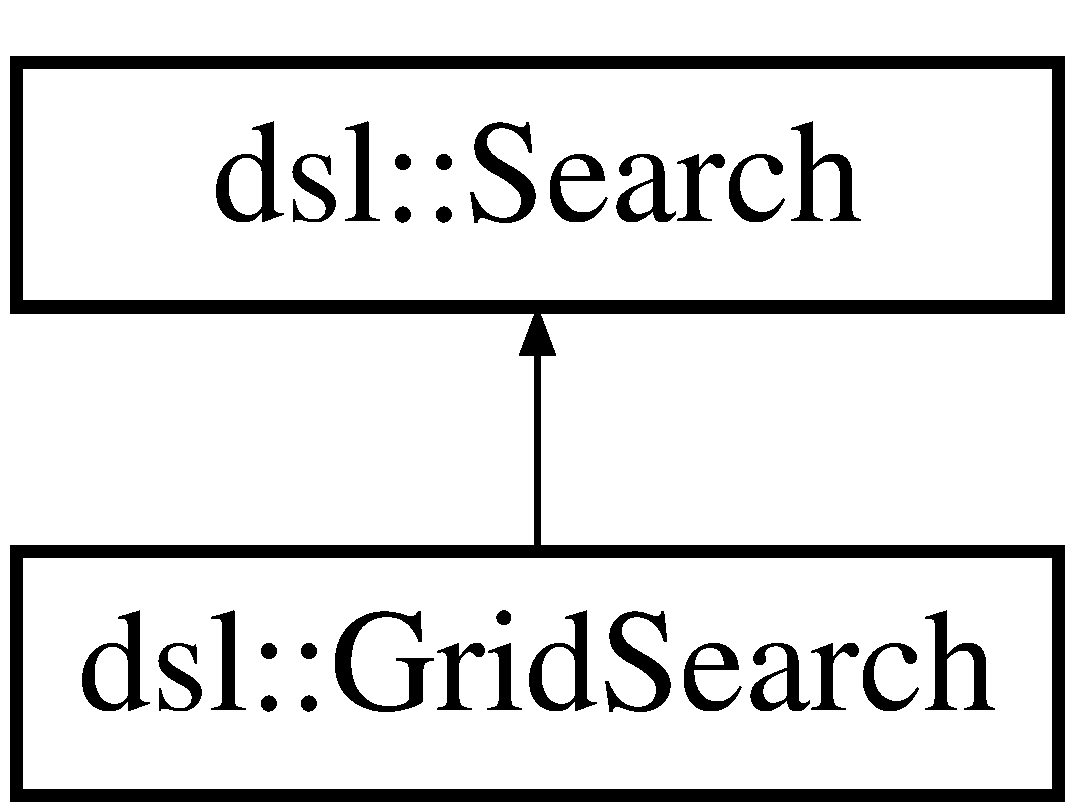
\includegraphics[height=2.000000cm]{classdsl_1_1GridSearch}
\end{center}
\end{figure}
\subsection*{Public Member Functions}
\begin{DoxyCompactItemize}
\item 
{\bf Grid\-Search} (int {\bf width}, int {\bf height}, const double $\ast${\bf map}=0, double {\bf scale}=1.\-0)
\item 
virtual {\bf $\sim$\-Grid\-Search} ()
\item 
void {\bf Set\-Cost} (int x, int y, double {\bf cost})
\item 
double {\bf Get\-Cost} (int x, int y) const 
\item 
void {\bf Set\-Map} (const double $\ast${\bf map})
\item 
void {\bf Set\-Start} (int x, int y)
\item 
void {\bf Set\-Goal} (int x, int y)
\item 
void {\bf Plan} ({\bf Grid\-Path} \&path)
\item 
void {\bf Opt\-Path} (const {\bf Grid\-Path} \&path, {\bf Grid\-Path} \&opt\-Path) const 
\item 
{\bf Vertex} $\ast$ {\bf Get\-Vertex} (int x, int y) const 
\item 
void {\bf Remove\-Vertex} (int x, int y)
\item 
void {\bf Add\-Edge} (int x1, int y1, int x2, int y2)
\end{DoxyCompactItemize}
\subsection*{Public Attributes}
\begin{DoxyCompactItemize}
\item 
int {\bf width}
\begin{DoxyCompactList}\small\item\em width of cost grid \end{DoxyCompactList}\item 
int {\bf height}
\begin{DoxyCompactList}\small\item\em height of cost grid \end{DoxyCompactList}\item 
double {\bf scale}
\begin{DoxyCompactList}\small\item\em scale of each cell cost and each transition cost \end{DoxyCompactList}\item 
double $\ast$ {\bf map}
\begin{DoxyCompactList}\small\item\em cost grid array of size width$\ast$height \end{DoxyCompactList}\end{DoxyCompactItemize}
\subsection*{Protected Attributes}
\begin{DoxyCompactItemize}
\item 
{\bf Graph} {\bf graph}
\item 
{\bf Grid\-Cost} {\bf cost}
\item 
{\bf Vertex} $\ast$$\ast$ {\bf vertex\-Map}
\begin{DoxyCompactList}\small\item\em vertex grid array of size width$\ast$height \end{DoxyCompactList}\end{DoxyCompactItemize}
\subsection*{Additional Inherited Members}


\subsection{Constructor \& Destructor Documentation}
\index{dsl\-::\-Grid\-Search@{dsl\-::\-Grid\-Search}!Grid\-Search@{Grid\-Search}}
\index{Grid\-Search@{Grid\-Search}!dsl::GridSearch@{dsl\-::\-Grid\-Search}}
\subsubsection[{Grid\-Search}]{\setlength{\rightskip}{0pt plus 5cm}Grid\-Search\-::\-Grid\-Search (
\begin{DoxyParamCaption}
\item[{int}]{width, }
\item[{int}]{height, }
\item[{const double $\ast$}]{map = {\ttfamily 0}, }
\item[{double}]{scale = {\ttfamily 1.0}}
\end{DoxyParamCaption}
)}\label{classdsl_1_1GridSearch_a088e396ffe2bc21376375bb5932d578f}
The planner allocates all states in the beginning a valid map of size width$\ast$height should be provided scale is used to multiply each cell value and each neighbor transition value before they are used for planning 
\begin{DoxyParams}{Parameters}
{\em width} & width \\
\hline
{\em height} & height \\
\hline
{\em map} & a double array of size width$\ast$height containing occupancy info (optional) \\
\hline
{\em scale} & the size of each cell (default is 1.\-0) \\
\hline
\end{DoxyParams}


References dsl\-::\-Graph\-::\-Add\-Edge(), dsl\-::\-Graph\-::\-Add\-Vertex(), graph, height, M\-A\-X, N\-B\-R\-\_\-\-C\-O\-U\-N\-T, vertex\-Map, and width.

\index{dsl\-::\-Grid\-Search@{dsl\-::\-Grid\-Search}!$\sim$\-Grid\-Search@{$\sim$\-Grid\-Search}}
\index{$\sim$\-Grid\-Search@{$\sim$\-Grid\-Search}!dsl::GridSearch@{dsl\-::\-Grid\-Search}}
\subsubsection[{$\sim$\-Grid\-Search}]{\setlength{\rightskip}{0pt plus 5cm}Grid\-Search\-::$\sim$\-Grid\-Search (
\begin{DoxyParamCaption}
{}
\end{DoxyParamCaption}
)\hspace{0.3cm}{\ttfamily [virtual]}}\label{classdsl_1_1GridSearch_a7c319016f2d53252109857aaca2b09d3}


References dsl\-::\-Vertex\-::data, height, map, vertex\-Map, and width.



\subsection{Member Function Documentation}
\index{dsl\-::\-Grid\-Search@{dsl\-::\-Grid\-Search}!Add\-Edge@{Add\-Edge}}
\index{Add\-Edge@{Add\-Edge}!dsl::GridSearch@{dsl\-::\-Grid\-Search}}
\subsubsection[{Add\-Edge}]{\setlength{\rightskip}{0pt plus 5cm}void Grid\-Search\-::\-Add\-Edge (
\begin{DoxyParamCaption}
\item[{int}]{x1, }
\item[{int}]{y1, }
\item[{int}]{x2, }
\item[{int}]{y2}
\end{DoxyParamCaption}
)}\label{classdsl_1_1GridSearch_a38bcbd68f597eda0a051f765e03b02fa}
Useful method for adding edges b/n vertices 
\begin{DoxyParams}{Parameters}
{\em x1} & from x-\/coordiante \\
\hline
{\em y1} & from y-\/coordiante \\
\hline
{\em x2} & to x-\/coordiante \\
\hline
{\em y2} & to y-\/coordiante \\
\hline
\end{DoxyParams}


References dsl\-::\-Graph\-::\-Add\-Edge(), Get\-Vertex(), and graph.

\index{dsl\-::\-Grid\-Search@{dsl\-::\-Grid\-Search}!Get\-Cost@{Get\-Cost}}
\index{Get\-Cost@{Get\-Cost}!dsl::GridSearch@{dsl\-::\-Grid\-Search}}
\subsubsection[{Get\-Cost}]{\setlength{\rightskip}{0pt plus 5cm}double Grid\-Search\-::\-Get\-Cost (
\begin{DoxyParamCaption}
\item[{int}]{x, }
\item[{int}]{y}
\end{DoxyParamCaption}
) const}\label{classdsl_1_1GridSearch_ac0f102bbb9cb82d6cc7c0b1760f7edca}
Get the cost of an individual cell 
\begin{DoxyParams}{Parameters}
{\em x} & x \\
\hline
{\em y} & y \\
\hline
\end{DoxyParams}
\begin{DoxyReturn}{Returns}
cost 
\end{DoxyReturn}


References map, and width.

\index{dsl\-::\-Grid\-Search@{dsl\-::\-Grid\-Search}!Get\-Vertex@{Get\-Vertex}}
\index{Get\-Vertex@{Get\-Vertex}!dsl::GridSearch@{dsl\-::\-Grid\-Search}}
\subsubsection[{Get\-Vertex}]{\setlength{\rightskip}{0pt plus 5cm}{\bf Vertex} $\ast$ Grid\-Search\-::\-Get\-Vertex (
\begin{DoxyParamCaption}
\item[{int}]{x, }
\item[{int}]{y}
\end{DoxyParamCaption}
) const}\label{classdsl_1_1GridSearch_a5ab3dea36f27a7d2c7ca4383e1e1b8e6}
Useful method to get the graph vertex at position (x,y) 
\begin{DoxyParams}{Parameters}
{\em x} & x-\/coordiante \\
\hline
{\em y} & y-\/coordiante \\
\hline
\end{DoxyParams}
\begin{DoxyReturn}{Returns}
corresponding vertex or 0 if none there 
\end{DoxyReturn}


References height, vertex\-Map, and width.



Referenced by Add\-Edge(), and Remove\-Vertex().

\index{dsl\-::\-Grid\-Search@{dsl\-::\-Grid\-Search}!Opt\-Path@{Opt\-Path}}
\index{Opt\-Path@{Opt\-Path}!dsl::GridSearch@{dsl\-::\-Grid\-Search}}
\subsubsection[{Opt\-Path}]{\setlength{\rightskip}{0pt plus 5cm}void Grid\-Search\-::\-Opt\-Path (
\begin{DoxyParamCaption}
\item[{const {\bf Grid\-Path} \&}]{path, }
\item[{{\bf Grid\-Path} \&}]{opt\-Path}
\end{DoxyParamCaption}
) const}\label{classdsl_1_1GridSearch_a8487c49c0c2a674a1b9fbe5fbdff643c}
Optimize the path produces by Plan 
\begin{DoxyParams}{Parameters}
{\em path} & an initial obstacle-\/free path (e.\-g. one produced by calling Plan(path)) \\
\hline
{\em opt\-Path} & a new path resulting from optimizing the original path path (i.\-e. a producing a shorter path with minimal number of obstacle-\/free segments) \\
\hline
\end{DoxyParams}


References dsl\-::\-Grid\-Path\-::count, dsl\-::\-Grid\-Path\-::len, map, dsl\-::\-Grid\-Path\-::pos, R\-A\-Y\-\_\-\-T\-R\-A\-C\-E\-\_\-\-S\-T\-E\-P, and width.



Referenced by main().

\index{dsl\-::\-Grid\-Search@{dsl\-::\-Grid\-Search}!Plan@{Plan}}
\index{Plan@{Plan}!dsl::GridSearch@{dsl\-::\-Grid\-Search}}
\subsubsection[{Plan}]{\setlength{\rightskip}{0pt plus 5cm}void Grid\-Search\-::\-Plan (
\begin{DoxyParamCaption}
\item[{{\bf Grid\-Path} \&}]{path}
\end{DoxyParamCaption}
)}\label{classdsl_1_1GridSearch_a529a35e2b3419c96dfbb7cbb5c39db32}
Compute path b/n start and goal vertices these vertices should be already set 
\begin{DoxyParams}{Parameters}
{\em path} & the resulting path \\
\hline
\end{DoxyParams}


References dsl\-::\-Grid\-Path\-::count, dsl\-::\-Vertex\-::data, dsl\-::\-Grid\-Path\-::len, dsl\-::\-Vertex\-::next, dsl\-::\-Search\-::\-Plan(), dsl\-::\-Grid\-Path\-::pos, and dsl\-::\-Search\-::start.



Referenced by main().

\index{dsl\-::\-Grid\-Search@{dsl\-::\-Grid\-Search}!Remove\-Vertex@{Remove\-Vertex}}
\index{Remove\-Vertex@{Remove\-Vertex}!dsl::GridSearch@{dsl\-::\-Grid\-Search}}
\subsubsection[{Remove\-Vertex}]{\setlength{\rightskip}{0pt plus 5cm}void Grid\-Search\-::\-Remove\-Vertex (
\begin{DoxyParamCaption}
\item[{int}]{x, }
\item[{int}]{y}
\end{DoxyParamCaption}
)}\label{classdsl_1_1GridSearch_a1f31b1d17ca13143bd44b145f0629f6e}
Useful method to remove a vertex at (x,y) 
\begin{DoxyParams}{Parameters}
{\em x} & x-\/coordiante \\
\hline
{\em y} & y-\/coordiante \\
\hline
\end{DoxyParams}


References Get\-Vertex(), graph, and dsl\-::\-Graph\-::\-Remove\-Vertex().



Referenced by main().

\index{dsl\-::\-Grid\-Search@{dsl\-::\-Grid\-Search}!Set\-Cost@{Set\-Cost}}
\index{Set\-Cost@{Set\-Cost}!dsl::GridSearch@{dsl\-::\-Grid\-Search}}
\subsubsection[{Set\-Cost}]{\setlength{\rightskip}{0pt plus 5cm}void Grid\-Search\-::\-Set\-Cost (
\begin{DoxyParamCaption}
\item[{int}]{x, }
\item[{int}]{y, }
\item[{double}]{cost}
\end{DoxyParamCaption}
)}\label{classdsl_1_1GridSearch_a46cb7bc7076b53cad44d3bb6e64b4909}
Change the cost of an individual cell 
\begin{DoxyParams}{Parameters}
{\em x} & x-\/coordinate \\
\hline
{\em y} & y-\/coordinate \\
\hline
{\em cost} & cost \\
\hline
\end{DoxyParams}


References dsl\-::\-Search\-::\-Change\-Cost(), cost, dsl\-::\-Search\-::\-Eq(), dsl\-::\-Vertex\-::in, map, dsl\-::\-Vertex\-::out, vertex\-Map, and width.



Referenced by main(), and Set\-Map().

\index{dsl\-::\-Grid\-Search@{dsl\-::\-Grid\-Search}!Set\-Goal@{Set\-Goal}}
\index{Set\-Goal@{Set\-Goal}!dsl::GridSearch@{dsl\-::\-Grid\-Search}}
\subsubsection[{Set\-Goal}]{\setlength{\rightskip}{0pt plus 5cm}void Grid\-Search\-::\-Set\-Goal (
\begin{DoxyParamCaption}
\item[{int}]{x, }
\item[{int}]{y}
\end{DoxyParamCaption}
)}\label{classdsl_1_1GridSearch_a033cfbe8313ee845f2c0dd8b5113fe6b}
Set goal location in the map 
\begin{DoxyParams}{Parameters}
{\em x} & x-\/coord \\
\hline
{\em y} & y-\/coord \\
\hline
\end{DoxyParams}


References dsl\-::\-Search\-::\-Set\-Goal(), vertex\-Map, and width.



Referenced by main().

\index{dsl\-::\-Grid\-Search@{dsl\-::\-Grid\-Search}!Set\-Map@{Set\-Map}}
\index{Set\-Map@{Set\-Map}!dsl::GridSearch@{dsl\-::\-Grid\-Search}}
\subsubsection[{Set\-Map}]{\setlength{\rightskip}{0pt plus 5cm}void Grid\-Search\-::\-Set\-Map (
\begin{DoxyParamCaption}
\item[{const double $\ast$}]{map}
\end{DoxyParamCaption}
)}\label{classdsl_1_1GridSearch_adbb22cd4bfb7f5d223d4f5ac4d5c2a60}
Change the costs of all cells at once 
\begin{DoxyParams}{Parameters}
{\em map} & a width$\ast$height double array containing occupancy data \\
\hline
\end{DoxyParams}


References height, Set\-Cost(), and width.

\index{dsl\-::\-Grid\-Search@{dsl\-::\-Grid\-Search}!Set\-Start@{Set\-Start}}
\index{Set\-Start@{Set\-Start}!dsl::GridSearch@{dsl\-::\-Grid\-Search}}
\subsubsection[{Set\-Start}]{\setlength{\rightskip}{0pt plus 5cm}void Grid\-Search\-::\-Set\-Start (
\begin{DoxyParamCaption}
\item[{int}]{x, }
\item[{int}]{y}
\end{DoxyParamCaption}
)}\label{classdsl_1_1GridSearch_a906aa657dffe9ee7a3d8f1493cf5889c}
Set start location in the map 
\begin{DoxyParams}{Parameters}
{\em x} & x-\/coord \\
\hline
{\em y} & y-\/coord \\
\hline
\end{DoxyParams}


References dsl\-::\-Search\-::\-Set\-Start(), vertex\-Map, and width.



Referenced by main().



\subsection{Member Data Documentation}
\index{dsl\-::\-Grid\-Search@{dsl\-::\-Grid\-Search}!cost@{cost}}
\index{cost@{cost}!dsl::GridSearch@{dsl\-::\-Grid\-Search}}
\subsubsection[{cost}]{\setlength{\rightskip}{0pt plus 5cm}{\bf Grid\-Cost} dsl\-::\-Grid\-Search\-::cost\hspace{0.3cm}{\ttfamily [protected]}}\label{classdsl_1_1GridSearch_ae4b06b2ddfc295598fcfe0da68f769ff}


Referenced by Set\-Cost().

\index{dsl\-::\-Grid\-Search@{dsl\-::\-Grid\-Search}!graph@{graph}}
\index{graph@{graph}!dsl::GridSearch@{dsl\-::\-Grid\-Search}}
\subsubsection[{graph}]{\setlength{\rightskip}{0pt plus 5cm}{\bf Graph} dsl\-::\-Grid\-Search\-::graph\hspace{0.3cm}{\ttfamily [protected]}}\label{classdsl_1_1GridSearch_ad465ba46be970dae903d4d1c5ad76e35}


Referenced by Add\-Edge(), Grid\-Search(), and Remove\-Vertex().

\index{dsl\-::\-Grid\-Search@{dsl\-::\-Grid\-Search}!height@{height}}
\index{height@{height}!dsl::GridSearch@{dsl\-::\-Grid\-Search}}
\subsubsection[{height}]{\setlength{\rightskip}{0pt plus 5cm}int dsl\-::\-Grid\-Search\-::height}\label{classdsl_1_1GridSearch_a765e59bd8afcd6cb983a9cee73d8ab12}


height of cost grid 



Referenced by Get\-Vertex(), Grid\-Search(), Set\-Map(), and $\sim$\-Grid\-Search().

\index{dsl\-::\-Grid\-Search@{dsl\-::\-Grid\-Search}!map@{map}}
\index{map@{map}!dsl::GridSearch@{dsl\-::\-Grid\-Search}}
\subsubsection[{map}]{\setlength{\rightskip}{0pt plus 5cm}double$\ast$ dsl\-::\-Grid\-Search\-::map}\label{classdsl_1_1GridSearch_acba55fef9aa96238a8047569b4c9aba0}


cost grid array of size width$\ast$height 



Referenced by Get\-Cost(), Opt\-Path(), Set\-Cost(), and $\sim$\-Grid\-Search().

\index{dsl\-::\-Grid\-Search@{dsl\-::\-Grid\-Search}!scale@{scale}}
\index{scale@{scale}!dsl::GridSearch@{dsl\-::\-Grid\-Search}}
\subsubsection[{scale}]{\setlength{\rightskip}{0pt plus 5cm}double dsl\-::\-Grid\-Search\-::scale}\label{classdsl_1_1GridSearch_af0815d65f819f2fb60d4e10b67c864f0}


scale of each cell cost and each transition cost 

\index{dsl\-::\-Grid\-Search@{dsl\-::\-Grid\-Search}!vertex\-Map@{vertex\-Map}}
\index{vertex\-Map@{vertex\-Map}!dsl::GridSearch@{dsl\-::\-Grid\-Search}}
\subsubsection[{vertex\-Map}]{\setlength{\rightskip}{0pt plus 5cm}{\bf Vertex}$\ast$$\ast$ dsl\-::\-Grid\-Search\-::vertex\-Map\hspace{0.3cm}{\ttfamily [protected]}}\label{classdsl_1_1GridSearch_aed8a4e7a0992fc9f9890b935a9182900}


vertex grid array of size width$\ast$height 



Referenced by Get\-Vertex(), Grid\-Search(), Set\-Cost(), Set\-Goal(), Set\-Start(), and $\sim$\-Grid\-Search().

\index{dsl\-::\-Grid\-Search@{dsl\-::\-Grid\-Search}!width@{width}}
\index{width@{width}!dsl::GridSearch@{dsl\-::\-Grid\-Search}}
\subsubsection[{width}]{\setlength{\rightskip}{0pt plus 5cm}int dsl\-::\-Grid\-Search\-::width}\label{classdsl_1_1GridSearch_a00f5f3859a75f31e0312697e702cfc98}


width of cost grid 



Referenced by Get\-Cost(), Get\-Vertex(), Grid\-Search(), Opt\-Path(), Set\-Cost(), Set\-Goal(), Set\-Map(), Set\-Start(), and $\sim$\-Grid\-Search().



The documentation for this class was generated from the following files\-:\begin{DoxyCompactItemize}
\item 
lib/{\bf gridsearch.\-h}\item 
lib/{\bf gridsearch.\-cc}\end{DoxyCompactItemize}

\section{dsl\-:\-:\-Grid\-Search3\-D \-Class \-Reference}
\label{classdsl_1_1GridSearch3D}\index{dsl\-::\-Grid\-Search3\-D@{dsl\-::\-Grid\-Search3\-D}}


{\ttfamily \#include $<$gridsearch3d.\-h$>$}

\-Inheritance diagram for dsl\-:\-:\-Grid\-Search3\-D\-:\begin{figure}[H]
\begin{center}
\leavevmode
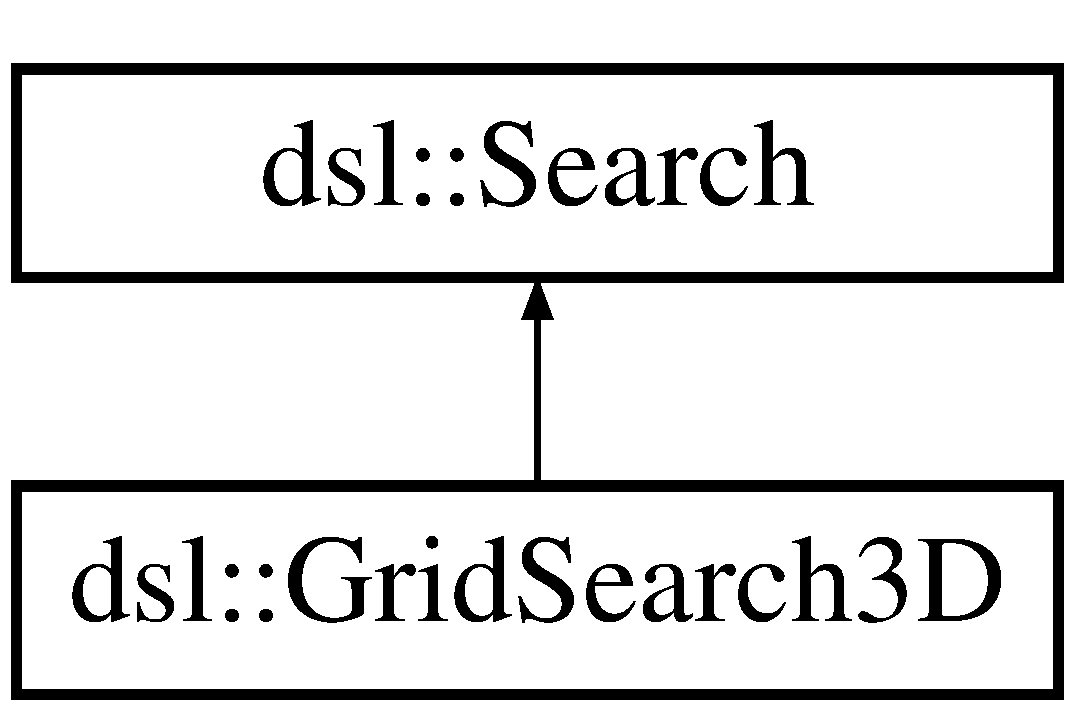
\includegraphics[height=2.000000cm]{classdsl_1_1GridSearch3D}
\end{center}
\end{figure}
\subsection*{\-Public \-Member \-Functions}
\begin{DoxyCompactItemize}
\item 
{\bf \-Grid\-Search3\-D} (int {\bf length}, int {\bf width}, int {\bf height}, const double $\ast${\bf map}=0, double {\bf scale}=1.\-0)
\item 
virtual {\bf $\sim$\-Grid\-Search3\-D} ()
\item 
void {\bf \-Set\-Cost} (int x, int y, int z, double {\bf cost})
\item 
double {\bf \-Get\-Cost} (int x, int y, int z) const 
\item 
void {\bf \-Set\-Map} (const double $\ast${\bf map})
\item 
void {\bf \-Set\-Start} (int x, int y, int z)
\item 
void {\bf \-Set\-Goal} (int x, int y, int z)
\item 
void {\bf \-Plan} ({\bf \-Grid\-Path3\-D} \&path)
\item 
void {\bf \-Opt\-Path} (const {\bf \-Grid\-Path3\-D} \&path, {\bf \-Grid\-Path3\-D} \&opt\-Path) const 
\item 
void {\bf \-Smooth\-Path\-Bezier} (const {\bf \-Grid\-Path3\-D} \&path, {\bf \-Grid\-Path3\-D} \&smooth\-Path, double smoothness) const 
\item 
void {\bf \-Smooth\-Path\-Spline} (const {\bf \-Grid\-Path3\-D} \&path, {\bf \-Grid\-Path3\-D\-Plus\-Time} \&smooth\-Path, double v, double time\-Step) const 
\item 
void {\bf \-Smooth\-Path\-Opt\-Cost} (const {\bf \-Grid\-Path3\-D} \&path, {\bf \-Grid\-Path3\-D\-Plus\-Time} \&smooth\-Path, double v, double time\-Step) const 
\item 
{\bf \-Vertex} $\ast$ {\bf \-Get\-Vertex} (int x, int y, int z) const 
\item 
void {\bf \-Remove\-Vertex} (int x, int y, int z)
\item 
void {\bf \-Add\-Edge} (int x1, int y1, int z1, int x2, int y2, int z2)
\end{DoxyCompactItemize}
\subsection*{\-Public \-Attributes}
\begin{DoxyCompactItemize}
\item 
int {\bf length}
\begin{DoxyCompactList}\small\item\em length of cost grid \end{DoxyCompactList}\item 
int {\bf width}
\begin{DoxyCompactList}\small\item\em width of cost grid \end{DoxyCompactList}\item 
int {\bf height}
\begin{DoxyCompactList}\small\item\em height of cost grid \end{DoxyCompactList}\item 
double {\bf scale}
\begin{DoxyCompactList}\small\item\em scale of each cell cost and each transition cost \end{DoxyCompactList}\item 
double $\ast$ {\bf map}
\begin{DoxyCompactList}\small\item\em cost grid array of size width$\ast$height \end{DoxyCompactList}\end{DoxyCompactItemize}
\subsection*{\-Protected \-Attributes}
\begin{DoxyCompactItemize}
\item 
{\bf \-Graph} {\bf graph}
\begin{DoxyCompactList}\small\item\em graph \end{DoxyCompactList}\item 
{\bf \-Grid\-Cost3\-D} {\bf cost}
\begin{DoxyCompactList}\small\item\em cost interface \end{DoxyCompactList}\item 
{\bf \-Vertex} $\ast$$\ast$ {\bf vertex\-Map}
\begin{DoxyCompactList}\small\item\em vertex grid array of size width$\ast$height \end{DoxyCompactList}\end{DoxyCompactItemize}


\subsection{\-Constructor \& \-Destructor \-Documentation}
\index{dsl\-::\-Grid\-Search3\-D@{dsl\-::\-Grid\-Search3\-D}!\-Grid\-Search3\-D@{\-Grid\-Search3\-D}}
\index{\-Grid\-Search3\-D@{\-Grid\-Search3\-D}!dsl::GridSearch3D@{dsl\-::\-Grid\-Search3\-D}}
\subsubsection[{\-Grid\-Search3\-D}]{\setlength{\rightskip}{0pt plus 5cm}{\bf \-Grid\-Search3\-D\-::\-Grid\-Search3\-D} (
\begin{DoxyParamCaption}
\item[{int}]{length, }
\item[{int}]{width, }
\item[{int}]{height, }
\item[{const double $\ast$}]{map = {\ttfamily 0}, }
\item[{double}]{scale = {\ttfamily 1.0}}
\end{DoxyParamCaption}
)}\label{classdsl_1_1GridSearch3D_a762887dcb2d68e006d85742861acbbe5}
\-The planner allocates all states in the beginning a valid map of size length$\ast$width$\ast$height should be provided scale is used to multiply each cell value and each neighbor transition value before they are used for planning 
\begin{DoxyParams}{\-Parameters}
{\em length} & length \\
\hline
{\em width} & width \\
\hline
{\em height} & height \\
\hline
{\em map} & a double array of size length$\ast$width$\ast$height containing occupancy info (optional) \\
\hline
{\em scale} & the size of each cell (default is 1.\-0) \\
\hline
\end{DoxyParams}


\-References dsl\-::\-Graph\-::\-Add\-Edge(), dsl\-::\-Graph\-::\-Add\-Vertex(), graph, height, length, \-M\-A\-X, \-N\-B\-R\-\_\-\-C\-O\-U\-N\-T, vertex\-Map, and width.

\index{dsl\-::\-Grid\-Search3\-D@{dsl\-::\-Grid\-Search3\-D}!$\sim$\-Grid\-Search3\-D@{$\sim$\-Grid\-Search3\-D}}
\index{$\sim$\-Grid\-Search3\-D@{$\sim$\-Grid\-Search3\-D}!dsl::GridSearch3D@{dsl\-::\-Grid\-Search3\-D}}
\subsubsection[{$\sim$\-Grid\-Search3\-D}]{\setlength{\rightskip}{0pt plus 5cm}{\bf \-Grid\-Search3\-D\-::$\sim$\-Grid\-Search3\-D} (
\begin{DoxyParamCaption}
{}
\end{DoxyParamCaption}
)\hspace{0.3cm}{\ttfamily  [virtual]}}\label{classdsl_1_1GridSearch3D_a07719281fe2ad4119f777c52432c81fb}


\-References dsl\-::\-Vertex\-::data, height, length, map, vertex\-Map, and width.



\subsection{\-Member \-Function \-Documentation}
\index{dsl\-::\-Grid\-Search3\-D@{dsl\-::\-Grid\-Search3\-D}!\-Add\-Edge@{\-Add\-Edge}}
\index{\-Add\-Edge@{\-Add\-Edge}!dsl::GridSearch3D@{dsl\-::\-Grid\-Search3\-D}}
\subsubsection[{\-Add\-Edge}]{\setlength{\rightskip}{0pt plus 5cm}void {\bf \-Grid\-Search3\-D\-::\-Add\-Edge} (
\begin{DoxyParamCaption}
\item[{int}]{x1, }
\item[{int}]{y1, }
\item[{int}]{z1, }
\item[{int}]{x2, }
\item[{int}]{y2, }
\item[{int}]{z2}
\end{DoxyParamCaption}
)}\label{classdsl_1_1GridSearch3D_a578583a53363ed7b5899eacfb7a09977}
\-Useful method for adding edges b/n vertices 
\begin{DoxyParams}{\-Parameters}
{\em x1} & from x-\/coordiante \\
\hline
{\em y1} & from y-\/coordiante \\
\hline
{\em z1} & from z-\/coordiante \\
\hline
{\em x2} & to x-\/coordiante \\
\hline
{\em y2} & to y-\/coordiante \\
\hline
{\em z2} & to z-\/coordiante \\
\hline
\end{DoxyParams}


\-References dsl\-::\-Graph\-::\-Add\-Edge(), \-Get\-Cost(), \-Get\-Vertex(), graph, \-M\-A\-X, and scale.

\index{dsl\-::\-Grid\-Search3\-D@{dsl\-::\-Grid\-Search3\-D}!\-Get\-Cost@{\-Get\-Cost}}
\index{\-Get\-Cost@{\-Get\-Cost}!dsl::GridSearch3D@{dsl\-::\-Grid\-Search3\-D}}
\subsubsection[{\-Get\-Cost}]{\setlength{\rightskip}{0pt plus 5cm}double {\bf \-Grid\-Search3\-D\-::\-Get\-Cost} (
\begin{DoxyParamCaption}
\item[{int}]{x, }
\item[{int}]{y, }
\item[{int}]{z}
\end{DoxyParamCaption}
) const}\label{classdsl_1_1GridSearch3D_a9f5b44270c3a100d44b11be3148a2436}
\-Get the cost of an individual cell 
\begin{DoxyParams}{\-Parameters}
{\em x} & x \\
\hline
{\em y} & y \\
\hline
{\em z} & z \\
\hline
\end{DoxyParams}
\begin{DoxyReturn}{\-Returns}
cost 
\end{DoxyReturn}


\-References \-D\-S\-L3\-D\-\_\-\-O\-C\-C\-U\-P\-I\-E\-D, height, length, map, and width.



\-Referenced by \-Add\-Edge(), \-Set\-Cost(), and \-Smooth\-Path\-Opt\-Cost().

\index{dsl\-::\-Grid\-Search3\-D@{dsl\-::\-Grid\-Search3\-D}!\-Get\-Vertex@{\-Get\-Vertex}}
\index{\-Get\-Vertex@{\-Get\-Vertex}!dsl::GridSearch3D@{dsl\-::\-Grid\-Search3\-D}}
\subsubsection[{\-Get\-Vertex}]{\setlength{\rightskip}{0pt plus 5cm}{\bf \-Vertex} $\ast$ {\bf \-Grid\-Search3\-D\-::\-Get\-Vertex} (
\begin{DoxyParamCaption}
\item[{int}]{x, }
\item[{int}]{y, }
\item[{int}]{z}
\end{DoxyParamCaption}
) const}\label{classdsl_1_1GridSearch3D_a6f29ccb57caab3966b4fa2abc737d171}
\-Useful method to get the graph vertex at position (x,y) 
\begin{DoxyParams}{\-Parameters}
{\em x} & x-\/coordinate \\
\hline
{\em y} & y-\/coordinate \\
\hline
{\em z} & z-\/coordinate \\
\hline
\end{DoxyParams}
\begin{DoxyReturn}{\-Returns}
corresponding vertex or 0 if none there 
\end{DoxyReturn}


\-References height, length, vertex\-Map, and width.



\-Referenced by \-Add\-Edge(), \-Remove\-Vertex(), \-Set\-Goal(), and \-Set\-Start().

\index{dsl\-::\-Grid\-Search3\-D@{dsl\-::\-Grid\-Search3\-D}!\-Opt\-Path@{\-Opt\-Path}}
\index{\-Opt\-Path@{\-Opt\-Path}!dsl::GridSearch3D@{dsl\-::\-Grid\-Search3\-D}}
\subsubsection[{\-Opt\-Path}]{\setlength{\rightskip}{0pt plus 5cm}void {\bf \-Grid\-Search3\-D\-::\-Opt\-Path} (
\begin{DoxyParamCaption}
\item[{const {\bf \-Grid\-Path3\-D} \&}]{path, }
\item[{{\bf \-Grid\-Path3\-D} \&}]{opt\-Path}
\end{DoxyParamCaption}
) const}\label{classdsl_1_1GridSearch3D_a9a2c518c60958e7a010fceeb3c45081b}
\-Optimize the path produced by \-Plan 
\begin{DoxyParams}{\-Parameters}
{\em path} & an initial obstacle-\/free path (e.\-g. one produced by calling \-Plan(path)) \\
\hline
{\em opt\-Path} & a new path resulting from optimizing the original path path (i.\-e. a producing a shorter path with minimal number of obstacle-\/free segments) \\
\hline
\end{DoxyParams}


\-References dsl\-::\-Grid\-Path3\-D\-::count, \-D\-S\-L3\-D\-\_\-\-O\-C\-C\-U\-P\-I\-E\-D, dsl\-::\-Grid\-Path3\-D\-::len, length, map, dsl\-::\-Grid\-Path3\-D\-::pos, \-R\-A\-Y\-\_\-\-T\-R\-A\-C\-E\-\_\-\-S\-T\-E\-P, and width.

\index{dsl\-::\-Grid\-Search3\-D@{dsl\-::\-Grid\-Search3\-D}!\-Plan@{\-Plan}}
\index{\-Plan@{\-Plan}!dsl::GridSearch3D@{dsl\-::\-Grid\-Search3\-D}}
\subsubsection[{\-Plan}]{\setlength{\rightskip}{0pt plus 5cm}void {\bf \-Grid\-Search3\-D\-::\-Plan} (
\begin{DoxyParamCaption}
\item[{{\bf \-Grid\-Path3\-D} \&}]{path}
\end{DoxyParamCaption}
)}\label{classdsl_1_1GridSearch3D_a64e2a08dc55d5cc13b8e4fc7fee574f6}
\-Compute path b/n start and goal vertices these vertices should be already set 
\begin{DoxyParams}{\-Parameters}
{\em path} & the resulting path \\
\hline
\end{DoxyParams}


\-References dsl\-::\-Grid\-Path3\-D\-::count, dsl\-::\-Vertex\-::data, dsl\-::\-Grid\-Path3\-D\-::len, dsl\-::\-Vertex\-::next, dsl\-::\-Search\-::\-Plan(), dsl\-::\-Grid\-Path3\-D\-::pos, and dsl\-::\-Search\-::start.

\index{dsl\-::\-Grid\-Search3\-D@{dsl\-::\-Grid\-Search3\-D}!\-Remove\-Vertex@{\-Remove\-Vertex}}
\index{\-Remove\-Vertex@{\-Remove\-Vertex}!dsl::GridSearch3D@{dsl\-::\-Grid\-Search3\-D}}
\subsubsection[{\-Remove\-Vertex}]{\setlength{\rightskip}{0pt plus 5cm}void {\bf \-Grid\-Search3\-D\-::\-Remove\-Vertex} (
\begin{DoxyParamCaption}
\item[{int}]{x, }
\item[{int}]{y, }
\item[{int}]{z}
\end{DoxyParamCaption}
)}\label{classdsl_1_1GridSearch3D_a531b957174801aba03df816858efdc79}
\-Useful method to remove a vertex at (x,y) 
\begin{DoxyParams}{\-Parameters}
{\em x} & x-\/coordinate \\
\hline
{\em y} & y-\/coordinate \\
\hline
{\em z} & z-\/coordinate \\
\hline
\end{DoxyParams}


\-References \-Get\-Vertex(), graph, and dsl\-::\-Graph\-::\-Remove\-Vertex().

\index{dsl\-::\-Grid\-Search3\-D@{dsl\-::\-Grid\-Search3\-D}!\-Set\-Cost@{\-Set\-Cost}}
\index{\-Set\-Cost@{\-Set\-Cost}!dsl::GridSearch3D@{dsl\-::\-Grid\-Search3\-D}}
\subsubsection[{\-Set\-Cost}]{\setlength{\rightskip}{0pt plus 5cm}void {\bf \-Grid\-Search3\-D\-::\-Set\-Cost} (
\begin{DoxyParamCaption}
\item[{int}]{x, }
\item[{int}]{y, }
\item[{int}]{z, }
\item[{double}]{cost}
\end{DoxyParamCaption}
)}\label{classdsl_1_1GridSearch3D_ab77662f0b4acac1831fa89251b19dc82}
\-Change the cost of an individual cell 
\begin{DoxyParams}{\-Parameters}
{\em x} & x-\/coordinate \\
\hline
{\em y} & y-\/coordinate \\
\hline
{\em z} & z-\/coordinate \\
\hline
{\em cost} & cost \\
\hline
\end{DoxyParams}


\-References dsl\-::\-Search\-::\-Change\-Cost(), cost, dsl\-::\-Search\-::\-Eq(), \-Get\-Cost(), dsl\-::\-Vertex\-::in, length, map, \-M\-A\-X, dsl\-::\-Vertex\-::out, scale, vertex\-Map, and width.



\-Referenced by \-Set\-Map().

\index{dsl\-::\-Grid\-Search3\-D@{dsl\-::\-Grid\-Search3\-D}!\-Set\-Goal@{\-Set\-Goal}}
\index{\-Set\-Goal@{\-Set\-Goal}!dsl::GridSearch3D@{dsl\-::\-Grid\-Search3\-D}}
\subsubsection[{\-Set\-Goal}]{\setlength{\rightskip}{0pt plus 5cm}void {\bf \-Grid\-Search3\-D\-::\-Set\-Goal} (
\begin{DoxyParamCaption}
\item[{int}]{x, }
\item[{int}]{y, }
\item[{int}]{z}
\end{DoxyParamCaption}
)}\label{classdsl_1_1GridSearch3D_a2ae259ead527bb1ce03e98537362a956}
\-Set goal location in the map 
\begin{DoxyParams}{\-Parameters}
{\em x} & x-\/coord \\
\hline
{\em y} & y-\/coord \\
\hline
{\em z} & z-\/coord \\
\hline
\end{DoxyParams}


\-References \-Get\-Vertex().

\index{dsl\-::\-Grid\-Search3\-D@{dsl\-::\-Grid\-Search3\-D}!\-Set\-Map@{\-Set\-Map}}
\index{\-Set\-Map@{\-Set\-Map}!dsl::GridSearch3D@{dsl\-::\-Grid\-Search3\-D}}
\subsubsection[{\-Set\-Map}]{\setlength{\rightskip}{0pt plus 5cm}void {\bf \-Grid\-Search3\-D\-::\-Set\-Map} (
\begin{DoxyParamCaption}
\item[{const double $\ast$}]{map}
\end{DoxyParamCaption}
)}\label{classdsl_1_1GridSearch3D_a11ead66a75931f61e5f1c37c6453688c}
\-Change the costs of all cells at once 
\begin{DoxyParams}{\-Parameters}
{\em map} & a length$\ast$width$\ast$height double array containing occupancy data \\
\hline
\end{DoxyParams}


\-References height, length, \-Set\-Cost(), and width.

\index{dsl\-::\-Grid\-Search3\-D@{dsl\-::\-Grid\-Search3\-D}!\-Set\-Start@{\-Set\-Start}}
\index{\-Set\-Start@{\-Set\-Start}!dsl::GridSearch3D@{dsl\-::\-Grid\-Search3\-D}}
\subsubsection[{\-Set\-Start}]{\setlength{\rightskip}{0pt plus 5cm}void {\bf \-Grid\-Search3\-D\-::\-Set\-Start} (
\begin{DoxyParamCaption}
\item[{int}]{x, }
\item[{int}]{y, }
\item[{int}]{z}
\end{DoxyParamCaption}
)}\label{classdsl_1_1GridSearch3D_a8781b974ca9a5729f37c3c4c2e580048}
\-Set start location in the map 
\begin{DoxyParams}{\-Parameters}
{\em x} & x-\/coord \\
\hline
{\em y} & y-\/coord \\
\hline
{\em z} & z-\/coord \\
\hline
\end{DoxyParams}


\-References \-Get\-Vertex().

\index{dsl\-::\-Grid\-Search3\-D@{dsl\-::\-Grid\-Search3\-D}!\-Smooth\-Path\-Bezier@{\-Smooth\-Path\-Bezier}}
\index{\-Smooth\-Path\-Bezier@{\-Smooth\-Path\-Bezier}!dsl::GridSearch3D@{dsl\-::\-Grid\-Search3\-D}}
\subsubsection[{\-Smooth\-Path\-Bezier}]{\setlength{\rightskip}{0pt plus 5cm}void {\bf \-Grid\-Search3\-D\-::\-Smooth\-Path\-Bezier} (
\begin{DoxyParamCaption}
\item[{const {\bf \-Grid\-Path3\-D} \&}]{path, }
\item[{{\bf \-Grid\-Path3\-D} \&}]{smooth\-Path, }
\item[{double}]{smoothness}
\end{DoxyParamCaption}
) const}\label{classdsl_1_1GridSearch3D_abb6fb1fb4c8d948e24d55b730a8fb9de}
\-Smooth the path produced by \-Plan with a \-Bezier interpolation 
\begin{DoxyParams}{\-Parameters}
{\em path} & an initial obstacle-\/free path (e.\-g. one produced by calling \-Plan(path)) \\
\hline
{\em opt\-Path} & a new path resulting from smoothing the original path path \\
\hline
{\em smoothness} & smoothness of the curve \\
\hline
\end{DoxyParams}


\-References dsl\-::\-Grid\-Path3\-D\-::count, dsl\-::\-Grid\-Path3\-D\-::len, dsl\-::\-Grid\-Path3\-D\-::pos, and \-R\-A\-Y\-\_\-\-T\-R\-A\-C\-E\-\_\-\-S\-T\-E\-P.

\index{dsl\-::\-Grid\-Search3\-D@{dsl\-::\-Grid\-Search3\-D}!\-Smooth\-Path\-Opt\-Cost@{\-Smooth\-Path\-Opt\-Cost}}
\index{\-Smooth\-Path\-Opt\-Cost@{\-Smooth\-Path\-Opt\-Cost}!dsl::GridSearch3D@{dsl\-::\-Grid\-Search3\-D}}
\subsubsection[{\-Smooth\-Path\-Opt\-Cost}]{\setlength{\rightskip}{0pt plus 5cm}void {\bf \-Grid\-Search3\-D\-::\-Smooth\-Path\-Opt\-Cost} (
\begin{DoxyParamCaption}
\item[{const {\bf \-Grid\-Path3\-D} \&}]{path, }
\item[{{\bf \-Grid\-Path3\-D\-Plus\-Time} \&}]{smooth\-Path, }
\item[{double}]{v, }
\item[{double}]{time\-Step}
\end{DoxyParamCaption}
) const}\label{classdsl_1_1GridSearch3D_a3636ee1303b1a8297bfd25c0322f1d8b}
\-Smooth the path produced by \-Plan with a clamped cubic spline, choosing the control points in order to minimize a cost function 
\begin{DoxyParams}{\-Parameters}
{\em path} & an initial obstacle-\/free path (e.\-g. one produced by calling \-Plan(path)) \\
\hline
{\em opt\-Path} & a new path resulting from smoothing the original path path \\
\hline
{\em v} & the average velocity along the path \\
\hline
{\em time\-Step} & the time between each point along the generated path \\
\hline
\end{DoxyParams}


\-References dsl\-::\-Grid\-Path3\-D\-::count, \-D\-S\-L3\-D\-\_\-\-O\-C\-C\-U\-P\-I\-E\-D, \-Get\-Cost(), dsl\-::\-Grid\-Path3\-D\-::len, dsl\-::\-Grid\-Path3\-D\-::pos, \-Smooth\-Path\-Spline(), and dsl\-::\-Grid\-Path3\-D\-Plus\-Time\-::times.

\index{dsl\-::\-Grid\-Search3\-D@{dsl\-::\-Grid\-Search3\-D}!\-Smooth\-Path\-Spline@{\-Smooth\-Path\-Spline}}
\index{\-Smooth\-Path\-Spline@{\-Smooth\-Path\-Spline}!dsl::GridSearch3D@{dsl\-::\-Grid\-Search3\-D}}
\subsubsection[{\-Smooth\-Path\-Spline}]{\setlength{\rightskip}{0pt plus 5cm}void {\bf \-Grid\-Search3\-D\-::\-Smooth\-Path\-Spline} (
\begin{DoxyParamCaption}
\item[{const {\bf \-Grid\-Path3\-D} \&}]{path, }
\item[{{\bf \-Grid\-Path3\-D\-Plus\-Time} \&}]{smooth\-Path, }
\item[{double}]{v, }
\item[{double}]{time\-Step}
\end{DoxyParamCaption}
) const}\label{classdsl_1_1GridSearch3D_aa33dc458fc2d145a18e2021e883c059a}
\-Smooth the path produced by \-Plan with a clamped cubic spline 
\begin{DoxyParams}{\-Parameters}
{\em path} & an initial obstacle-\/free path (e.\-g. one produced by calling \-Plan(path)) \\
\hline
{\em opt\-Path} & a new path resulting from smoothing the original path path \\
\hline
{\em v} & the average velocity along the path \\
\hline
{\em time\-Step} & the time between each point along the generated path \\
\hline
\end{DoxyParams}


\-References dsl\-::\-Grid\-Path3\-D\-::count, dsl\-::\-Grid\-Path3\-D\-::len, dsl\-::\-Grid\-Path3\-D\-::pos, and dsl\-::\-Grid\-Path3\-D\-Plus\-Time\-::times.



\-Referenced by \-Smooth\-Path\-Opt\-Cost().



\subsection{\-Member \-Data \-Documentation}
\index{dsl\-::\-Grid\-Search3\-D@{dsl\-::\-Grid\-Search3\-D}!cost@{cost}}
\index{cost@{cost}!dsl::GridSearch3D@{dsl\-::\-Grid\-Search3\-D}}
\subsubsection[{cost}]{\setlength{\rightskip}{0pt plus 5cm}{\bf \-Grid\-Cost3\-D} {\bf dsl\-::\-Grid\-Search3\-D\-::cost}\hspace{0.3cm}{\ttfamily  [protected]}}\label{classdsl_1_1GridSearch3D_afdd94f2e7d091f11cbdaf1b171847222}


cost interface 



\-Reimplemented from {\bf dsl\-::\-Search} \doxyref{}{p.}{classdsl_1_1Search_af6c350062139fd6d0887c4dd6de40d75}.



\-Referenced by \-Set\-Cost().

\index{dsl\-::\-Grid\-Search3\-D@{dsl\-::\-Grid\-Search3\-D}!graph@{graph}}
\index{graph@{graph}!dsl::GridSearch3D@{dsl\-::\-Grid\-Search3\-D}}
\subsubsection[{graph}]{\setlength{\rightskip}{0pt plus 5cm}{\bf \-Graph} {\bf dsl\-::\-Grid\-Search3\-D\-::graph}\hspace{0.3cm}{\ttfamily  [protected]}}\label{classdsl_1_1GridSearch3D_a37f3c79462ee3df5bfa525744f206ea3}


graph 



\-Reimplemented from {\bf dsl\-::\-Search} \doxyref{}{p.}{classdsl_1_1Search_a41367e4af253eeb3aad5deaac1e31753}.



\-Referenced by \-Add\-Edge(), \-Grid\-Search3\-D(), and \-Remove\-Vertex().

\index{dsl\-::\-Grid\-Search3\-D@{dsl\-::\-Grid\-Search3\-D}!height@{height}}
\index{height@{height}!dsl::GridSearch3D@{dsl\-::\-Grid\-Search3\-D}}
\subsubsection[{height}]{\setlength{\rightskip}{0pt plus 5cm}int {\bf dsl\-::\-Grid\-Search3\-D\-::height}}\label{classdsl_1_1GridSearch3D_a1b2e431cf22e53adb72733d59432ad97}


height of cost grid 



\-Referenced by \-Get\-Cost(), \-Get\-Vertex(), \-Grid\-Search3\-D(), \-Set\-Map(), and $\sim$\-Grid\-Search3\-D().

\index{dsl\-::\-Grid\-Search3\-D@{dsl\-::\-Grid\-Search3\-D}!length@{length}}
\index{length@{length}!dsl::GridSearch3D@{dsl\-::\-Grid\-Search3\-D}}
\subsubsection[{length}]{\setlength{\rightskip}{0pt plus 5cm}int {\bf dsl\-::\-Grid\-Search3\-D\-::length}}\label{classdsl_1_1GridSearch3D_abed307ca7dc5c270ef4069c5450c57a4}


length of cost grid 



\-Referenced by \-Get\-Cost(), \-Get\-Vertex(), \-Grid\-Search3\-D(), \-Opt\-Path(), \-Set\-Cost(), \-Set\-Map(), and $\sim$\-Grid\-Search3\-D().

\index{dsl\-::\-Grid\-Search3\-D@{dsl\-::\-Grid\-Search3\-D}!map@{map}}
\index{map@{map}!dsl::GridSearch3D@{dsl\-::\-Grid\-Search3\-D}}
\subsubsection[{map}]{\setlength{\rightskip}{0pt plus 5cm}double$\ast$ {\bf dsl\-::\-Grid\-Search3\-D\-::map}}\label{classdsl_1_1GridSearch3D_a9525be96df6595e5788c2933c71302e8}


cost grid array of size width$\ast$height 



\-Referenced by \-Get\-Cost(), \-Opt\-Path(), \-Set\-Cost(), and $\sim$\-Grid\-Search3\-D().

\index{dsl\-::\-Grid\-Search3\-D@{dsl\-::\-Grid\-Search3\-D}!scale@{scale}}
\index{scale@{scale}!dsl::GridSearch3D@{dsl\-::\-Grid\-Search3\-D}}
\subsubsection[{scale}]{\setlength{\rightskip}{0pt plus 5cm}double {\bf dsl\-::\-Grid\-Search3\-D\-::scale}}\label{classdsl_1_1GridSearch3D_ab46d8bcfd681739d7e06409a5043aa0b}


scale of each cell cost and each transition cost 



\-Referenced by \-Add\-Edge(), and \-Set\-Cost().

\index{dsl\-::\-Grid\-Search3\-D@{dsl\-::\-Grid\-Search3\-D}!vertex\-Map@{vertex\-Map}}
\index{vertex\-Map@{vertex\-Map}!dsl::GridSearch3D@{dsl\-::\-Grid\-Search3\-D}}
\subsubsection[{vertex\-Map}]{\setlength{\rightskip}{0pt plus 5cm}{\bf \-Vertex}$\ast$$\ast$ {\bf dsl\-::\-Grid\-Search3\-D\-::vertex\-Map}\hspace{0.3cm}{\ttfamily  [protected]}}\label{classdsl_1_1GridSearch3D_aebca7498409019fc176a87643850bc7e}


vertex grid array of size width$\ast$height 



\-Referenced by \-Get\-Vertex(), \-Grid\-Search3\-D(), \-Set\-Cost(), and $\sim$\-Grid\-Search3\-D().

\index{dsl\-::\-Grid\-Search3\-D@{dsl\-::\-Grid\-Search3\-D}!width@{width}}
\index{width@{width}!dsl::GridSearch3D@{dsl\-::\-Grid\-Search3\-D}}
\subsubsection[{width}]{\setlength{\rightskip}{0pt plus 5cm}int {\bf dsl\-::\-Grid\-Search3\-D\-::width}}\label{classdsl_1_1GridSearch3D_a43aec353e9eb9aeafbd5623c0dc53ded}


width of cost grid 



\-Referenced by \-Get\-Cost(), \-Get\-Vertex(), \-Grid\-Search3\-D(), \-Opt\-Path(), \-Set\-Cost(), \-Set\-Map(), and $\sim$\-Grid\-Search3\-D().



\-The documentation for this class was generated from the following files\-:\begin{DoxyCompactItemize}
\item 
/home/matt/dsl/lib/{\bf gridsearch3d.\-h}\item 
/home/matt/dsl/lib/{\bf gridsearch3d.\-cc}\end{DoxyCompactItemize}

\section{dsl\-:\-:\-Search \-Class \-Reference}
\label{classdsl_1_1Search}\index{dsl\-::\-Search@{dsl\-::\-Search}}


{\ttfamily \#include $<$search.\-h$>$}

\-Inheritance diagram for dsl\-:\-:\-Search\-:\begin{figure}[H]
\begin{center}
\leavevmode
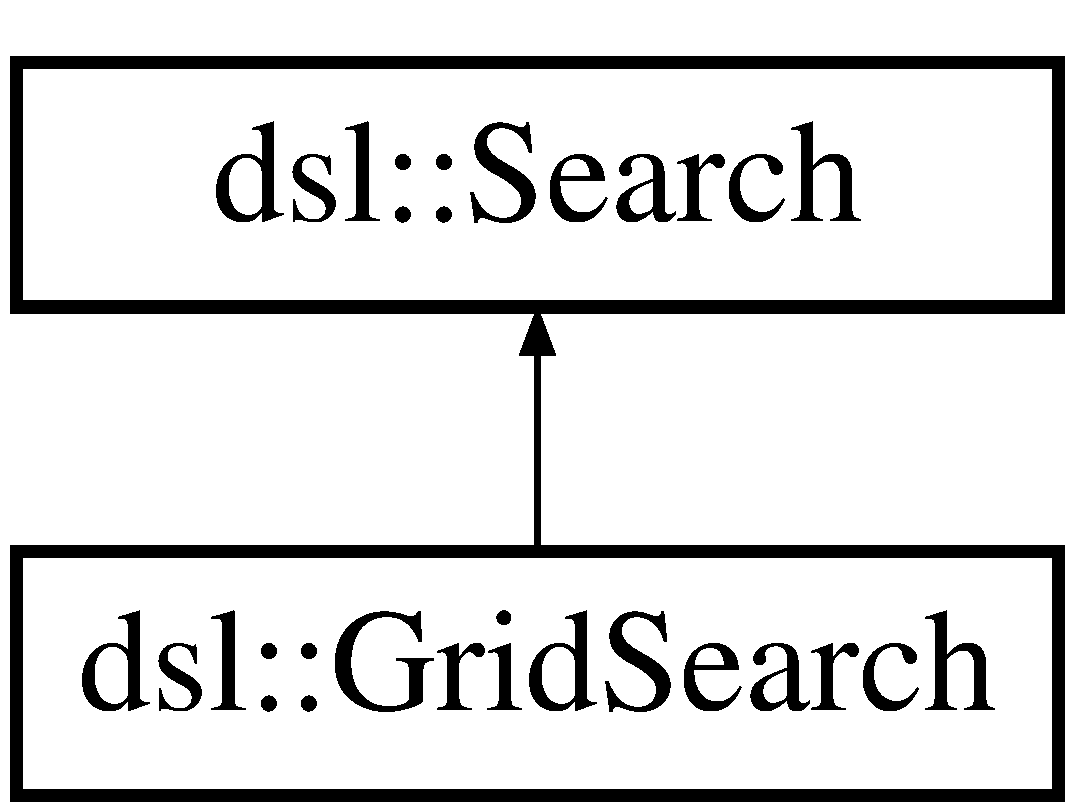
\includegraphics[height=3.000000cm]{classdsl_1_1Search}
\end{center}
\end{figure}
\subsection*{\-Public \-Member \-Functions}
\begin{DoxyCompactItemize}
\item 
{\bf \-Search} ({\bf \-Graph} \&{\bf graph}, const {\bf \-Cost} \&{\bf cost})
\item 
virtual {\bf $\sim$\-Search} ()
\item 
void {\bf \-Reset} ()
\item 
int {\bf \-Plan} ()
\item 
void {\bf \-Set\-Start} (const {\bf \-Vertex} \&v)
\item 
void {\bf \-Set\-Goal} (const {\bf \-Vertex} \&v)
\item 
void {\bf \-Change\-Cost} ({\bf \-Edge} \&e, double {\bf cost})
\item 
void {\bf \-Set\-Eps} (double {\bf eps})
\end{DoxyCompactItemize}
\subsection*{\-Protected \-Member \-Functions}
\begin{DoxyCompactItemize}
\item 
void {\bf \-Update\-Vertex} ({\bf \-Vertex} \&u)
\item 
void {\bf \-Compute\-Shortest\-Path} ()
\item 
{\bf \-Vertex} $\ast$ {\bf \-Min\-Succ} (double $\ast$min\-Rhs, const {\bf \-Vertex} \&v)
\item 
double $\ast$ {\bf \-Calculate\-Ext\-Key} (double $\ast$key, {\bf \-Vertex} \&v)
\item 
double $\ast$ {\bf \-Calculate\-Key} ({\bf \-Vertex} \&v)
\item 
void {\bf \-Insert} ({\bf \-Vertex} \&v)
\item 
void {\bf \-Insert\-Ext} ({\bf \-Vertex} \&v, double $\ast$key)
\item 
void {\bf \-Update} ({\bf \-Vertex} \&v)
\item 
void {\bf \-Remove} ({\bf \-Vertex} \&v)
\item 
{\bf \-Vertex} $\ast$ {\bf \-Pop} ()
\item 
{\bf \-Vertex} $\ast$ {\bf \-Top} ()
\item 
double $\ast$ {\bf \-Top\-Key} ()
\item 
bool {\bf \-Eq} (double a, double b) const 
\end{DoxyCompactItemize}
\subsection*{\-Protected \-Attributes}
\begin{DoxyCompactItemize}
\item 
{\bf \-Graph} \& {\bf graph}
\begin{DoxyCompactList}\small\item\em graph \end{DoxyCompactList}\item 
const {\bf \-Cost} \& {\bf cost}
\begin{DoxyCompactList}\small\item\em cost interface \end{DoxyCompactList}\item 
std\-::vector$<$ {\bf \-Edge} $\ast$ $>$ {\bf changed\-Edges}
\begin{DoxyCompactList}\small\item\em newly changed edges \end{DoxyCompactList}\item 
{\bf \-Vertex} $\ast$ {\bf start}
\begin{DoxyCompactList}\small\item\em start state \end{DoxyCompactList}\item 
{\bf \-Vertex} $\ast$ {\bf goal}
\begin{DoxyCompactList}\small\item\em goal state \end{DoxyCompactList}\item 
{\bf \-Vertex} $\ast$ {\bf last}
\begin{DoxyCompactList}\small\item\em last state \end{DoxyCompactList}\item 
double {\bf km}
\begin{DoxyCompactList}\small\item\em km variable \end{DoxyCompactList}\item 
fibheap\-\_\-t {\bf open\-List}
\begin{DoxyCompactList}\small\item\em fibonacci heap \end{DoxyCompactList}\item 
double {\bf eps}
\begin{DoxyCompactList}\small\item\em epsilon for cost comparision \end{DoxyCompactList}\end{DoxyCompactItemize}
\subsection*{\-Friends}
\begin{DoxyCompactItemize}
\item 
class {\bf \-Graph}
\end{DoxyCompactItemize}


\subsection{\-Constructor \& \-Destructor \-Documentation}
\index{dsl\-::\-Search@{dsl\-::\-Search}!\-Search@{\-Search}}
\index{\-Search@{\-Search}!dsl::Search@{dsl\-::\-Search}}
\subsubsection[{\-Search}]{\setlength{\rightskip}{0pt plus 5cm}{\bf \-Search\-::\-Search} (
\begin{DoxyParamCaption}
\item[{{\bf \-Graph} \&}]{graph, }
\item[{const {\bf \-Cost} \&}]{cost}
\end{DoxyParamCaption}
)}\label{classdsl_1_1Search_a558d369dc90bdfc0f4ad5a7350926082}
\-Initialize dsl with a graph and a cost interface 
\begin{DoxyParams}{\-Parameters}
{\em graph} & graph (the method will modify the nodes in the graph by changing certain search-\/related parameters stored at the nodes, the data or the original edge costs would not be changed) \\
\hline
{\em cost} & cost interface \\
\hline
\end{DoxyParams}


\-References open\-List.

\index{dsl\-::\-Search@{dsl\-::\-Search}!$\sim$\-Search@{$\sim$\-Search}}
\index{$\sim$\-Search@{$\sim$\-Search}!dsl::Search@{dsl\-::\-Search}}
\subsubsection[{$\sim$\-Search}]{\setlength{\rightskip}{0pt plus 5cm}{\bf \-Search\-::$\sim$\-Search} (
\begin{DoxyParamCaption}
{}
\end{DoxyParamCaption}
)\hspace{0.3cm}{\ttfamily  [virtual]}}\label{classdsl_1_1Search_afd7e16f7369d7a44189e530292b5faa0}


\-References changed\-Edges, and open\-List.



\subsection{\-Member \-Function \-Documentation}
\index{dsl\-::\-Search@{dsl\-::\-Search}!\-Calculate\-Ext\-Key@{\-Calculate\-Ext\-Key}}
\index{\-Calculate\-Ext\-Key@{\-Calculate\-Ext\-Key}!dsl::Search@{dsl\-::\-Search}}
\subsubsection[{\-Calculate\-Ext\-Key}]{\setlength{\rightskip}{0pt plus 5cm}double $\ast$ {\bf \-Search\-::\-Calculate\-Ext\-Key} (
\begin{DoxyParamCaption}
\item[{double $\ast$}]{key, }
\item[{{\bf \-Vertex} \&}]{v}
\end{DoxyParamCaption}
)\hspace{0.3cm}{\ttfamily  [protected]}}\label{classdsl_1_1Search_a6e602d83bffee7fad9e3bb9f02eb107b}


\-References cost, \-D\-S\-L\-\_\-\-M\-I\-N, dsl\-::\-Vertex\-::g, dsl\-::\-Cost\-::\-Heur(), \-I\-N\-F, km, dsl\-::\-Vertex\-::rhs, and start.



\-Referenced by \-Calculate\-Key(), \-Insert(), and \-Update().

\index{dsl\-::\-Search@{dsl\-::\-Search}!\-Calculate\-Key@{\-Calculate\-Key}}
\index{\-Calculate\-Key@{\-Calculate\-Key}!dsl::Search@{dsl\-::\-Search}}
\subsubsection[{\-Calculate\-Key}]{\setlength{\rightskip}{0pt plus 5cm}double $\ast$ {\bf \-Search\-::\-Calculate\-Key} (
\begin{DoxyParamCaption}
\item[{{\bf \-Vertex} \&}]{v}
\end{DoxyParamCaption}
)\hspace{0.3cm}{\ttfamily  [protected]}}\label{classdsl_1_1Search_ad59c81421975e3f3855100f73e8e6f17}


\-References \-Calculate\-Ext\-Key(), and dsl\-::\-Vertex\-::key.



\-Referenced by \-Compute\-Shortest\-Path().

\index{dsl\-::\-Search@{dsl\-::\-Search}!\-Change\-Cost@{\-Change\-Cost}}
\index{\-Change\-Cost@{\-Change\-Cost}!dsl::Search@{dsl\-::\-Search}}
\subsubsection[{\-Change\-Cost}]{\setlength{\rightskip}{0pt plus 5cm}void {\bf \-Search\-::\-Change\-Cost} (
\begin{DoxyParamCaption}
\item[{{\bf \-Edge} \&}]{e, }
\item[{double}]{cost}
\end{DoxyParamCaption}
)}\label{classdsl_1_1Search_aa4633ccb38de011506d12c63b1dcf8a9}
\-Change the cost of edge e 
\begin{DoxyParams}{\-Parameters}
{\em e} & edge \\
\hline
{\em cost} & new cost \\
\hline
\end{DoxyParams}


\-References changed\-Edges, dsl\-::\-Edge\-::cost, cost, dsl\-::\-Edge\-::cost\-Change, and \-Eq().



\-Referenced by dsl\-::\-Graph\-::\-Add\-Edge(), dsl\-::\-Grid\-Search\-::\-Set\-Cost(), and dsl\-::\-Grid\-Search3\-D\-::\-Set\-Cost().

\index{dsl\-::\-Search@{dsl\-::\-Search}!\-Compute\-Shortest\-Path@{\-Compute\-Shortest\-Path}}
\index{\-Compute\-Shortest\-Path@{\-Compute\-Shortest\-Path}!dsl::Search@{dsl\-::\-Search}}
\subsubsection[{\-Compute\-Shortest\-Path}]{\setlength{\rightskip}{0pt plus 5cm}void {\bf \-Search\-::\-Compute\-Shortest\-Path} (
\begin{DoxyParamCaption}
{}
\end{DoxyParamCaption}
)\hspace{0.3cm}{\ttfamily  [protected]}}\label{classdsl_1_1Search_a214747a0309d0ba593964bbf2244e0f6}


\-References \-Calculate\-Key(), dsl\-::\-Edge\-::cost, \-D\-S\-L\-\_\-\-M\-I\-N, \-Eq(), fibkey\-\_\-compare(), dsl\-::\-Edge\-::from, dsl\-::\-Vertex\-::g, goal, graph, dsl\-::\-Vertex\-::in, \-I\-N\-F, dsl\-::\-Vertex\-::key, \-Min\-Succ(), open\-List, \-Remove(), dsl\-::\-Vertex\-::rhs, dsl\-::\-Graph\-::search, start, \-Top(), \-Top\-Key(), \-Update(), and \-Update\-Vertex().



\-Referenced by \-Plan().

\index{dsl\-::\-Search@{dsl\-::\-Search}!\-Eq@{\-Eq}}
\index{\-Eq@{\-Eq}!dsl::Search@{dsl\-::\-Search}}
\subsubsection[{\-Eq}]{\setlength{\rightskip}{0pt plus 5cm}bool {\bf dsl\-::\-Search\-::\-Eq} (
\begin{DoxyParamCaption}
\item[{double}]{a, }
\item[{double}]{b}
\end{DoxyParamCaption}
) const\hspace{0.3cm}{\ttfamily  [inline, protected]}}\label{classdsl_1_1Search_a97cf2c2745ef182fd27e99fadf0e7650}
\-Compare two doubles for equality 
\begin{DoxyParams}{\-Parameters}
{\em a} & first number \\
\hline
{\em b} & second number \\
\hline
\end{DoxyParams}
\begin{DoxyReturn}{\-Returns}
$|a-b| < eps$ 
\end{DoxyReturn}


\-References eps.



\-Referenced by \-Change\-Cost(), \-Compute\-Shortest\-Path(), \-Plan(), dsl\-::\-Graph\-::\-Remove\-Edge(), dsl\-::\-Grid\-Search\-::\-Set\-Cost(), and dsl\-::\-Grid\-Search3\-D\-::\-Set\-Cost().

\index{dsl\-::\-Search@{dsl\-::\-Search}!\-Insert@{\-Insert}}
\index{\-Insert@{\-Insert}!dsl::Search@{dsl\-::\-Search}}
\subsubsection[{\-Insert}]{\setlength{\rightskip}{0pt plus 5cm}void {\bf \-Search\-::\-Insert} (
\begin{DoxyParamCaption}
\item[{{\bf \-Vertex} \&}]{v}
\end{DoxyParamCaption}
)\hspace{0.3cm}{\ttfamily  [protected]}}\label{classdsl_1_1Search_a32e20777f1d5b600172c5d95198aeabf}


\-References \-Calculate\-Ext\-Key(), \-Insert\-Ext(), and dsl\-::\-Vertex\-::key.



\-Referenced by \-Update\-Vertex().

\index{dsl\-::\-Search@{dsl\-::\-Search}!\-Insert\-Ext@{\-Insert\-Ext}}
\index{\-Insert\-Ext@{\-Insert\-Ext}!dsl::Search@{dsl\-::\-Search}}
\subsubsection[{\-Insert\-Ext}]{\setlength{\rightskip}{0pt plus 5cm}void {\bf \-Search\-::\-Insert\-Ext} (
\begin{DoxyParamCaption}
\item[{{\bf \-Vertex} \&}]{v, }
\item[{double $\ast$}]{key}
\end{DoxyParamCaption}
)\hspace{0.3cm}{\ttfamily  [protected]}}\label{classdsl_1_1Search_a8bd2f838ecad2222cb74a7c4e8c4641b}


\-References dsl\-::\-Vertex\-::\-O\-P\-E\-N, open\-List, dsl\-::\-Vertex\-::open\-List\-Node, start, and dsl\-::\-Vertex\-::t.



\-Referenced by \-Insert(), and \-Set\-Goal().

\index{dsl\-::\-Search@{dsl\-::\-Search}!\-Min\-Succ@{\-Min\-Succ}}
\index{\-Min\-Succ@{\-Min\-Succ}!dsl::Search@{dsl\-::\-Search}}
\subsubsection[{\-Min\-Succ}]{\setlength{\rightskip}{0pt plus 5cm}{\bf \-Vertex} $\ast$ {\bf \-Search\-::\-Min\-Succ} (
\begin{DoxyParamCaption}
\item[{double $\ast$}]{min\-Rhs, }
\item[{const {\bf \-Vertex} \&}]{v}
\end{DoxyParamCaption}
)\hspace{0.3cm}{\ttfamily  [protected]}}\label{classdsl_1_1Search_a7f097eaacb5f0e0425a979df873848f9}


\-References dsl\-::\-Edge\-::cost, cost, dsl\-::\-Vertex\-::g, goal, \-I\-N\-F, dsl\-::\-Vertex\-::out, dsl\-::\-Cost\-::\-Real(), and dsl\-::\-Edge\-::to.



\-Referenced by \-Compute\-Shortest\-Path(), \-Plan(), and dsl\-::\-Graph\-::\-Remove\-Edge().

\index{dsl\-::\-Search@{dsl\-::\-Search}!\-Plan@{\-Plan}}
\index{\-Plan@{\-Plan}!dsl::Search@{dsl\-::\-Search}}
\subsubsection[{\-Plan}]{\setlength{\rightskip}{0pt plus 5cm}int {\bf \-Search\-::\-Plan} (
\begin{DoxyParamCaption}
{}
\end{DoxyParamCaption}
)}\label{classdsl_1_1Search_ab4424706f45fda5a280d40ce4ea0ce31}
\-Plan an initial path from start to goal, or if any cost changes are detected since it was last called (any calls to \doxyref{\-Change\-Cost()}{p.}{classdsl_1_1Search_aa4633ccb38de011506d12c63b1dcf8a9}) then it replans. \-The generated path can be obtained by following the next pointers from start vertex until goal vertex is reached \begin{DoxyReturn}{\-Returns}
total number of vertices along the path 
\end{DoxyReturn}


\-References changed\-Edges, \-Compute\-Shortest\-Path(), dsl\-::\-Edge\-::cost, cost, dsl\-::\-Edge\-::cost\-Change, \-D\-S\-L\-\_\-\-M\-I\-N, \-Eq(), dsl\-::\-Edge\-::from, dsl\-::\-Vertex\-::g, goal, dsl\-::\-Cost\-::\-Heur(), dsl\-::\-Vertex\-::in, km, last, \-Min\-Succ(), dsl\-::\-Vertex\-::next, dsl\-::\-Vertex\-::out, dsl\-::\-Vertex\-::prev, dsl\-::\-Vertex\-::rhs, start, dsl\-::\-Edge\-::to, and \-Update\-Vertex().



\-Referenced by dsl\-::\-Grid\-Search\-::\-Plan(), and dsl\-::\-Grid\-Search3\-D\-::\-Plan().

\index{dsl\-::\-Search@{dsl\-::\-Search}!\-Pop@{\-Pop}}
\index{\-Pop@{\-Pop}!dsl::Search@{dsl\-::\-Search}}
\subsubsection[{\-Pop}]{\setlength{\rightskip}{0pt plus 5cm}{\bf \-Vertex} $\ast$ {\bf \-Search\-::\-Pop} (
\begin{DoxyParamCaption}
{}
\end{DoxyParamCaption}
)\hspace{0.3cm}{\ttfamily  [protected]}}\label{classdsl_1_1Search_a4844b3dad869bd250f54ab2f2f0d781a}
\index{dsl\-::\-Search@{dsl\-::\-Search}!\-Remove@{\-Remove}}
\index{\-Remove@{\-Remove}!dsl::Search@{dsl\-::\-Search}}
\subsubsection[{\-Remove}]{\setlength{\rightskip}{0pt plus 5cm}void {\bf \-Search\-::\-Remove} (
\begin{DoxyParamCaption}
\item[{{\bf \-Vertex} \&}]{v}
\end{DoxyParamCaption}
)\hspace{0.3cm}{\ttfamily  [protected]}}\label{classdsl_1_1Search_adbcedeafed6eee6e07d17084aedbb935}


\-References dsl\-::\-Vertex\-::\-C\-L\-O\-S\-E\-D, open\-List, dsl\-::\-Vertex\-::open\-List\-Node, and dsl\-::\-Vertex\-::t.



\-Referenced by \-Compute\-Shortest\-Path(), dsl\-::\-Graph\-::\-Remove\-Vertex(), and \-Update\-Vertex().

\index{dsl\-::\-Search@{dsl\-::\-Search}!\-Reset@{\-Reset}}
\index{\-Reset@{\-Reset}!dsl::Search@{dsl\-::\-Search}}
\subsubsection[{\-Reset}]{\setlength{\rightskip}{0pt plus 5cm}void {\bf \-Search\-::\-Reset} (
\begin{DoxyParamCaption}
{}
\end{DoxyParamCaption}
)}\label{classdsl_1_1Search_a869532b31ac40a532e00348b3199c0fa}
\-Reset the planner to its initial state this can be used for example if the goal state was changed but the graph structure is the same \-This is usually called internally at init and with every \doxyref{\-Set\-Goal()}{p.}{classdsl_1_1Search_ac3553c27300a5a3cdefb821de8681523} 

\-References graph, km, last, open\-List, and dsl\-::\-Graph\-::vertices.



\-Referenced by \-Set\-Goal().

\index{dsl\-::\-Search@{dsl\-::\-Search}!\-Set\-Eps@{\-Set\-Eps}}
\index{\-Set\-Eps@{\-Set\-Eps}!dsl::Search@{dsl\-::\-Search}}
\subsubsection[{\-Set\-Eps}]{\setlength{\rightskip}{0pt plus 5cm}void {\bf dsl\-::\-Search\-::\-Set\-Eps} (
\begin{DoxyParamCaption}
\item[{double}]{eps}
\end{DoxyParamCaption}
)\hspace{0.3cm}{\ttfamily  [inline]}}\label{classdsl_1_1Search_a1f458b3b02d08ef931fd2134be39c954}
\-Set epsilon\-: this is used to compare cell costs 
\begin{DoxyParams}{\-Parameters}
{\em eps} & precision (1e-\/10 by default) \\
\hline
\end{DoxyParams}


\-References eps.

\index{dsl\-::\-Search@{dsl\-::\-Search}!\-Set\-Goal@{\-Set\-Goal}}
\index{\-Set\-Goal@{\-Set\-Goal}!dsl::Search@{dsl\-::\-Search}}
\subsubsection[{\-Set\-Goal}]{\setlength{\rightskip}{0pt plus 5cm}void {\bf \-Search\-::\-Set\-Goal} (
\begin{DoxyParamCaption}
\item[{const {\bf \-Vertex} \&}]{v}
\end{DoxyParamCaption}
)}\label{classdsl_1_1Search_ac3553c27300a5a3cdefb821de8681523}
\-Set goal state this also resets the planner 
\begin{DoxyParams}{\-Parameters}
{\em v} & goal vertex \\
\hline
\end{DoxyParams}


\-References cost, goal, dsl\-::\-Cost\-::\-Heur(), \-Insert\-Ext(), dsl\-::\-Vertex\-::key, \-Reset(), dsl\-::\-Vertex\-::rhs, and start.

\index{dsl\-::\-Search@{dsl\-::\-Search}!\-Set\-Start@{\-Set\-Start}}
\index{\-Set\-Start@{\-Set\-Start}!dsl::Search@{dsl\-::\-Search}}
\subsubsection[{\-Set\-Start}]{\setlength{\rightskip}{0pt plus 5cm}void {\bf \-Search\-::\-Set\-Start} (
\begin{DoxyParamCaption}
\item[{const {\bf \-Vertex} \&}]{v}
\end{DoxyParamCaption}
)}\label{classdsl_1_1Search_a85d5cad5f6f79100e695afda95072fc7}
\-Set start state 
\begin{DoxyParams}{\-Parameters}
{\em v} & start vertex \\
\hline
\end{DoxyParams}


\-References start.

\index{dsl\-::\-Search@{dsl\-::\-Search}!\-Top@{\-Top}}
\index{\-Top@{\-Top}!dsl::Search@{dsl\-::\-Search}}
\subsubsection[{\-Top}]{\setlength{\rightskip}{0pt plus 5cm}{\bf \-Vertex} $\ast$ {\bf \-Search\-::\-Top} (
\begin{DoxyParamCaption}
{}
\end{DoxyParamCaption}
)\hspace{0.3cm}{\ttfamily  [protected]}}\label{classdsl_1_1Search_a9c6a4de62e5a58e3d24f4ba513c61a8c}


\-References open\-List, start, and \-Update().



\-Referenced by \-Compute\-Shortest\-Path(), and \-Top\-Key().

\index{dsl\-::\-Search@{dsl\-::\-Search}!\-Top\-Key@{\-Top\-Key}}
\index{\-Top\-Key@{\-Top\-Key}!dsl::Search@{dsl\-::\-Search}}
\subsubsection[{\-Top\-Key}]{\setlength{\rightskip}{0pt plus 5cm}double $\ast$ {\bf \-Search\-::\-Top\-Key} (
\begin{DoxyParamCaption}
{}
\end{DoxyParamCaption}
)\hspace{0.3cm}{\ttfamily  [protected]}}\label{classdsl_1_1Search_a7f629e92b0410574823c96b0b6cea8fe}


\-References dsl\-::\-Vertex\-::key, and \-Top().



\-Referenced by \-Compute\-Shortest\-Path().

\index{dsl\-::\-Search@{dsl\-::\-Search}!\-Update@{\-Update}}
\index{\-Update@{\-Update}!dsl::Search@{dsl\-::\-Search}}
\subsubsection[{\-Update}]{\setlength{\rightskip}{0pt plus 5cm}void {\bf \-Search\-::\-Update} (
\begin{DoxyParamCaption}
\item[{{\bf \-Vertex} \&}]{v}
\end{DoxyParamCaption}
)\hspace{0.3cm}{\ttfamily  [protected]}}\label{classdsl_1_1Search_a444dd522438619227fc157382723c3a6}


\-References \-Calculate\-Ext\-Key(), fibkey\-\_\-compare(), dsl\-::\-Vertex\-::key, dsl\-::\-Vertex\-::\-O\-P\-E\-N, open\-List, dsl\-::\-Vertex\-::open\-List\-Node, start, and dsl\-::\-Vertex\-::t.



\-Referenced by \-Compute\-Shortest\-Path(), \-Top(), and \-Update\-Vertex().

\index{dsl\-::\-Search@{dsl\-::\-Search}!\-Update\-Vertex@{\-Update\-Vertex}}
\index{\-Update\-Vertex@{\-Update\-Vertex}!dsl::Search@{dsl\-::\-Search}}
\subsubsection[{\-Update\-Vertex}]{\setlength{\rightskip}{0pt plus 5cm}void {\bf \-Search\-::\-Update\-Vertex} (
\begin{DoxyParamCaption}
\item[{{\bf \-Vertex} \&}]{u}
\end{DoxyParamCaption}
)\hspace{0.3cm}{\ttfamily  [protected]}}\label{classdsl_1_1Search_a6667ab42755828ca578ff9411c158145}


\-References dsl\-::\-Vertex\-::g, \-Insert(), dsl\-::\-Vertex\-::\-O\-P\-E\-N, \-Remove(), dsl\-::\-Vertex\-::rhs, dsl\-::\-Vertex\-::t, and \-Update().



\-Referenced by \-Compute\-Shortest\-Path(), \-Plan(), and dsl\-::\-Graph\-::\-Remove\-Edge().



\subsection{\-Friends \-And \-Related \-Function \-Documentation}
\index{dsl\-::\-Search@{dsl\-::\-Search}!\-Graph@{\-Graph}}
\index{\-Graph@{\-Graph}!dsl::Search@{dsl\-::\-Search}}
\subsubsection[{\-Graph}]{\setlength{\rightskip}{0pt plus 5cm}friend class {\bf \-Graph}\hspace{0.3cm}{\ttfamily  [friend]}}\label{classdsl_1_1Search_afab89afd724f1b07b1aaad6bdc61c47a}


\subsection{\-Member \-Data \-Documentation}
\index{dsl\-::\-Search@{dsl\-::\-Search}!changed\-Edges@{changed\-Edges}}
\index{changed\-Edges@{changed\-Edges}!dsl::Search@{dsl\-::\-Search}}
\subsubsection[{changed\-Edges}]{\setlength{\rightskip}{0pt plus 5cm}std\-::vector$<${\bf \-Edge}$\ast$$>$ {\bf dsl\-::\-Search\-::changed\-Edges}\hspace{0.3cm}{\ttfamily  [protected]}}\label{classdsl_1_1Search_aa82b611625b3ca55bc9b2e9f8fb20148}


newly changed edges 



\-Referenced by \-Change\-Cost(), \-Plan(), and $\sim$\-Search().

\index{dsl\-::\-Search@{dsl\-::\-Search}!cost@{cost}}
\index{cost@{cost}!dsl::Search@{dsl\-::\-Search}}
\subsubsection[{cost}]{\setlength{\rightskip}{0pt plus 5cm}const {\bf \-Cost}\& {\bf dsl\-::\-Search\-::cost}\hspace{0.3cm}{\ttfamily  [protected]}}\label{classdsl_1_1Search_af6c350062139fd6d0887c4dd6de40d75}


cost interface 



\-Reimplemented in {\bf dsl\-::\-Grid\-Search3\-D} \doxyref{}{p.}{classdsl_1_1GridSearch3D_afdd94f2e7d091f11cbdaf1b171847222}, and {\bf dsl\-::\-Grid\-Search} \doxyref{}{p.}{classdsl_1_1GridSearch_ae4b06b2ddfc295598fcfe0da68f769ff}.



\-Referenced by \-Calculate\-Ext\-Key(), \-Change\-Cost(), \-Min\-Succ(), \-Plan(), and \-Set\-Goal().

\index{dsl\-::\-Search@{dsl\-::\-Search}!eps@{eps}}
\index{eps@{eps}!dsl::Search@{dsl\-::\-Search}}
\subsubsection[{eps}]{\setlength{\rightskip}{0pt plus 5cm}double {\bf dsl\-::\-Search\-::eps}\hspace{0.3cm}{\ttfamily  [protected]}}\label{classdsl_1_1Search_a2c4ab71403607a88a8eaf3ec550b86cd}


epsilon for cost comparision 



\-Referenced by \-Eq(), and \-Set\-Eps().

\index{dsl\-::\-Search@{dsl\-::\-Search}!goal@{goal}}
\index{goal@{goal}!dsl::Search@{dsl\-::\-Search}}
\subsubsection[{goal}]{\setlength{\rightskip}{0pt plus 5cm}{\bf \-Vertex}$\ast$ {\bf dsl\-::\-Search\-::goal}\hspace{0.3cm}{\ttfamily  [protected]}}\label{classdsl_1_1Search_a8c625a87603367abf735c587bce06e0d}


goal state 



\-Referenced by \-Compute\-Shortest\-Path(), \-Min\-Succ(), \-Plan(), dsl\-::\-Graph\-::\-Remove\-Edge(), and \-Set\-Goal().

\index{dsl\-::\-Search@{dsl\-::\-Search}!graph@{graph}}
\index{graph@{graph}!dsl::Search@{dsl\-::\-Search}}
\subsubsection[{graph}]{\setlength{\rightskip}{0pt plus 5cm}{\bf \-Graph}\& {\bf dsl\-::\-Search\-::graph}\hspace{0.3cm}{\ttfamily  [protected]}}\label{classdsl_1_1Search_a41367e4af253eeb3aad5deaac1e31753}


graph 



\-Reimplemented in {\bf dsl\-::\-Grid\-Search3\-D} \doxyref{}{p.}{classdsl_1_1GridSearch3D_a37f3c79462ee3df5bfa525744f206ea3}, and {\bf dsl\-::\-Grid\-Search} \doxyref{}{p.}{classdsl_1_1GridSearch_ad465ba46be970dae903d4d1c5ad76e35}.



\-Referenced by \-Compute\-Shortest\-Path(), and \-Reset().

\index{dsl\-::\-Search@{dsl\-::\-Search}!km@{km}}
\index{km@{km}!dsl::Search@{dsl\-::\-Search}}
\subsubsection[{km}]{\setlength{\rightskip}{0pt plus 5cm}double {\bf dsl\-::\-Search\-::km}\hspace{0.3cm}{\ttfamily  [protected]}}\label{classdsl_1_1Search_ae85ce3ec7324f0f80350cb403db6170a}


km variable 



\-Referenced by \-Calculate\-Ext\-Key(), \-Plan(), and \-Reset().

\index{dsl\-::\-Search@{dsl\-::\-Search}!last@{last}}
\index{last@{last}!dsl::Search@{dsl\-::\-Search}}
\subsubsection[{last}]{\setlength{\rightskip}{0pt plus 5cm}{\bf \-Vertex}$\ast$ {\bf dsl\-::\-Search\-::last}\hspace{0.3cm}{\ttfamily  [protected]}}\label{classdsl_1_1Search_a1ae57feeea79f31010b43f3b0488e910}


last state 



\-Referenced by dsl\-::\-Graph\-::\-Add\-Edge(), \-Plan(), dsl\-::\-Graph\-::\-Remove\-Edge(), dsl\-::\-Graph\-::\-Remove\-Vertex(), and \-Reset().

\index{dsl\-::\-Search@{dsl\-::\-Search}!open\-List@{open\-List}}
\index{open\-List@{open\-List}!dsl::Search@{dsl\-::\-Search}}
\subsubsection[{open\-List}]{\setlength{\rightskip}{0pt plus 5cm}fibheap\-\_\-t {\bf dsl\-::\-Search\-::open\-List}\hspace{0.3cm}{\ttfamily  [protected]}}\label{classdsl_1_1Search_ae6bf8ace708ddd7beab48d3784b62d79}


fibonacci heap 



\-Referenced by \-Compute\-Shortest\-Path(), \-Insert\-Ext(), \-Remove(), \-Reset(), \-Search(), \-Top(), \-Update(), and $\sim$\-Search().

\index{dsl\-::\-Search@{dsl\-::\-Search}!start@{start}}
\index{start@{start}!dsl::Search@{dsl\-::\-Search}}
\subsubsection[{start}]{\setlength{\rightskip}{0pt plus 5cm}{\bf \-Vertex}$\ast$ {\bf dsl\-::\-Search\-::start}\hspace{0.3cm}{\ttfamily  [protected]}}\label{classdsl_1_1Search_acabfc7913a140a3cc263dd5338d705ae}


start state 



\-Referenced by \-Calculate\-Ext\-Key(), \-Compute\-Shortest\-Path(), \-Insert\-Ext(), dsl\-::\-Grid\-Search\-::\-Plan(), \-Plan(), dsl\-::\-Grid\-Search3\-D\-::\-Plan(), \-Set\-Goal(), \-Set\-Start(), \-Top(), and \-Update().



\-The documentation for this class was generated from the following files\-:\begin{DoxyCompactItemize}
\item 
/home/matt/dsl/lib/{\bf search.\-h}\item 
/home/matt/dsl/lib/{\bf search.\-cc}\end{DoxyCompactItemize}

\section{\-Spline$<$ \-X, \-Y $>$ \-Class \-Template \-Reference}
\label{classSpline}\index{\-Spline$<$ X, Y $>$@{\-Spline$<$ X, Y $>$}}


{\ttfamily \#include $<$spline.\-h$>$}

\subsection*{\-Classes}
\begin{DoxyCompactItemize}
\item 
class {\bf \-Element}
\end{DoxyCompactItemize}
\subsection*{\-Public \-Member \-Functions}
\begin{DoxyCompactItemize}
\item 
{\bf \-Spline} ()
\item 
{\bf \-Spline} (const std\-::vector$<$ \-X $>$ \&x, const std\-::vector$<$ \-Y $>$ \&y)
\item 
virtual {\bf $\sim$\-Spline} ()
\item 
\-Y {\bf operator[$\,$]} (const \-X \&x) const 
\item 
\-Y {\bf interpolate} (const \-X \&x) const 
\item 
std\-::vector$<$ \-Y $>$ {\bf operator[$\,$]} (const std\-::vector$<$ \-X $>$ \&xx) const 
\item 
std\-::vector$<$ \-Y $>$ {\bf interpolate} (const std\-::vector$<$ \-X $>$ \&xx) const 
\end{DoxyCompactItemize}
\subsection*{\-Protected \-Types}
\begin{DoxyCompactItemize}
\item 
typedef {\bf \-Element} {\bf element\-\_\-type}
\end{DoxyCompactItemize}
\subsection*{\-Protected \-Attributes}
\begin{DoxyCompactItemize}
\item 
std\-::vector$<$ {\bf element\-\_\-type} $>$ {\bf m\-Elements}
\end{DoxyCompactItemize}


\subsection{\-Detailed \-Description}
\subsubsection*{template$<$typename \-X, typename \-Y$>$class Spline$<$ X, Y $>$}

\-Templated on type of \-X, \-Y. \-X and \-Y must have operator +, -\/, $\ast$, /. \-Y must have defined a constructor that takes a scalar. 

\subsection{\-Member \-Typedef \-Documentation}
\index{\-Spline@{\-Spline}!element\-\_\-type@{element\-\_\-type}}
\index{element\-\_\-type@{element\-\_\-type}!Spline@{\-Spline}}
\subsubsection[{element\-\_\-type}]{\setlength{\rightskip}{0pt plus 5cm}template$<$typename \-X, typename \-Y$>$ typedef {\bf \-Element} {\bf \-Spline}$<$ \-X, \-Y $>$\-::{\bf element\-\_\-type}\hspace{0.3cm}{\ttfamily  [protected]}}\label{classSpline_a0e5f568df00822e6467ad4b6ae6907f1}


\subsection{\-Constructor \& \-Destructor \-Documentation}
\index{\-Spline@{\-Spline}!\-Spline@{\-Spline}}
\index{\-Spline@{\-Spline}!Spline@{\-Spline}}
\subsubsection[{\-Spline}]{\setlength{\rightskip}{0pt plus 5cm}template$<$typename \-X, typename \-Y$>$ {\bf \-Spline}$<$ \-X, \-Y $>$\-::{\bf \-Spline} (
\begin{DoxyParamCaption}
{}
\end{DoxyParamCaption}
)\hspace{0.3cm}{\ttfamily  [inline]}}\label{classSpline_ac97ca6fde5f351cbe739a291de6cfa40}
\-An empty, invalid spline \index{\-Spline@{\-Spline}!\-Spline@{\-Spline}}
\index{\-Spline@{\-Spline}!Spline@{\-Spline}}
\subsubsection[{\-Spline}]{\setlength{\rightskip}{0pt plus 5cm}template$<$typename \-X, typename \-Y$>$ {\bf \-Spline}$<$ \-X, \-Y $>$\-::{\bf \-Spline} (
\begin{DoxyParamCaption}
\item[{const std\-::vector$<$ \-X $>$ \&}]{x, }
\item[{const std\-::vector$<$ \-Y $>$ \&}]{y}
\end{DoxyParamCaption}
)\hspace{0.3cm}{\ttfamily  [inline]}}\label{classSpline_a9202b2897674c1877b2287f83a3079e9}
\-A spline with x and y values 

\-References \-Spline$<$ X, Y $>$\-::m\-Elements.

\index{\-Spline@{\-Spline}!$\sim$\-Spline@{$\sim$\-Spline}}
\index{$\sim$\-Spline@{$\sim$\-Spline}!Spline@{\-Spline}}
\subsubsection[{$\sim$\-Spline}]{\setlength{\rightskip}{0pt plus 5cm}template$<$typename \-X, typename \-Y$>$ virtual {\bf \-Spline}$<$ \-X, \-Y $>$\-::$\sim${\bf \-Spline} (
\begin{DoxyParamCaption}
{}
\end{DoxyParamCaption}
)\hspace{0.3cm}{\ttfamily  [inline, virtual]}}\label{classSpline_a4345b257b90292036e0a4cc2809ddac1}


\subsection{\-Member \-Function \-Documentation}
\index{\-Spline@{\-Spline}!interpolate@{interpolate}}
\index{interpolate@{interpolate}!Spline@{\-Spline}}
\subsubsection[{interpolate}]{\setlength{\rightskip}{0pt plus 5cm}template$<$typename \-X, typename \-Y$>$ \-Y {\bf \-Spline}$<$ \-X, \-Y $>$\-::{\bf interpolate} (
\begin{DoxyParamCaption}
\item[{const \-X \&}]{x}
\end{DoxyParamCaption}
) const\hspace{0.3cm}{\ttfamily  [inline]}}\label{classSpline_ad8594d762a6673e573d38aba5bef70ec}


\-References \-Spline$<$ X, Y $>$\-::m\-Elements.



\-Referenced by \-Spline$<$ X, Y $>$\-::operator[$\,$]().

\index{\-Spline@{\-Spline}!interpolate@{interpolate}}
\index{interpolate@{interpolate}!Spline@{\-Spline}}
\subsubsection[{interpolate}]{\setlength{\rightskip}{0pt plus 5cm}template$<$typename \-X, typename \-Y$>$ std\-::vector$<$\-Y$>$ {\bf \-Spline}$<$ \-X, \-Y $>$\-::{\bf interpolate} (
\begin{DoxyParamCaption}
\item[{const std\-::vector$<$ \-X $>$ \&}]{xx}
\end{DoxyParamCaption}
) const\hspace{0.3cm}{\ttfamily  [inline]}}\label{classSpline_aec162530d74514a6bc57d1cd8d7fe116}


\-References \-Spline$<$ X, Y $>$\-::m\-Elements.

\index{\-Spline@{\-Spline}!operator[$\,$]@{operator[]}}
\index{operator[$\,$]@{operator[]}!Spline@{\-Spline}}
\subsubsection[{operator[]}]{\setlength{\rightskip}{0pt plus 5cm}template$<$typename \-X, typename \-Y$>$ \-Y {\bf \-Spline}$<$ \-X, \-Y $>$\-::operator[$\,$] (
\begin{DoxyParamCaption}
\item[{const \-X \&}]{x}
\end{DoxyParamCaption}
) const\hspace{0.3cm}{\ttfamily  [inline]}}\label{classSpline_a52fd94178e1e0cb612bdb018acc1fee6}


\-References \-Spline$<$ X, Y $>$\-::interpolate().

\index{\-Spline@{\-Spline}!operator[$\,$]@{operator[]}}
\index{operator[$\,$]@{operator[]}!Spline@{\-Spline}}
\subsubsection[{operator[]}]{\setlength{\rightskip}{0pt plus 5cm}template$<$typename \-X, typename \-Y$>$ std\-::vector$<$\-Y$>$ {\bf \-Spline}$<$ \-X, \-Y $>$\-::operator[$\,$] (
\begin{DoxyParamCaption}
\item[{const std\-::vector$<$ \-X $>$ \&}]{xx}
\end{DoxyParamCaption}
) const\hspace{0.3cm}{\ttfamily  [inline]}}\label{classSpline_abdd648dce89434bacb38309eadf13106}


\-References \-Spline$<$ X, Y $>$\-::interpolate().



\subsection{\-Member \-Data \-Documentation}
\index{\-Spline@{\-Spline}!m\-Elements@{m\-Elements}}
\index{m\-Elements@{m\-Elements}!Spline@{\-Spline}}
\subsubsection[{m\-Elements}]{\setlength{\rightskip}{0pt plus 5cm}template$<$typename \-X, typename \-Y$>$ std\-::vector$<${\bf element\-\_\-type}$>$ {\bf \-Spline}$<$ \-X, \-Y $>$\-::{\bf m\-Elements}\hspace{0.3cm}{\ttfamily  [protected]}}\label{classSpline_aec12d605758ea834a7de781781de7e95}


\-Referenced by \-Spline$<$ X, Y $>$\-::interpolate(), and \-Spline$<$ X, Y $>$\-::\-Spline().



\-The documentation for this class was generated from the following file\-:\begin{DoxyCompactItemize}
\item 
/home/matt/dsl/lib/{\bf spline.\-h}\end{DoxyCompactItemize}

\section{dsl\-:\-:\-Trav\-Edge\-Cost \-Class \-Reference}
\label{classdsl_1_1TravEdgeCost}\index{dsl\-::\-Trav\-Edge\-Cost@{dsl\-::\-Trav\-Edge\-Cost}}


{\ttfamily \#include $<$travedgecost.\-h$>$}

\-Inheritance diagram for dsl\-:\-:\-Trav\-Edge\-Cost\-:\begin{figure}[H]
\begin{center}
\leavevmode
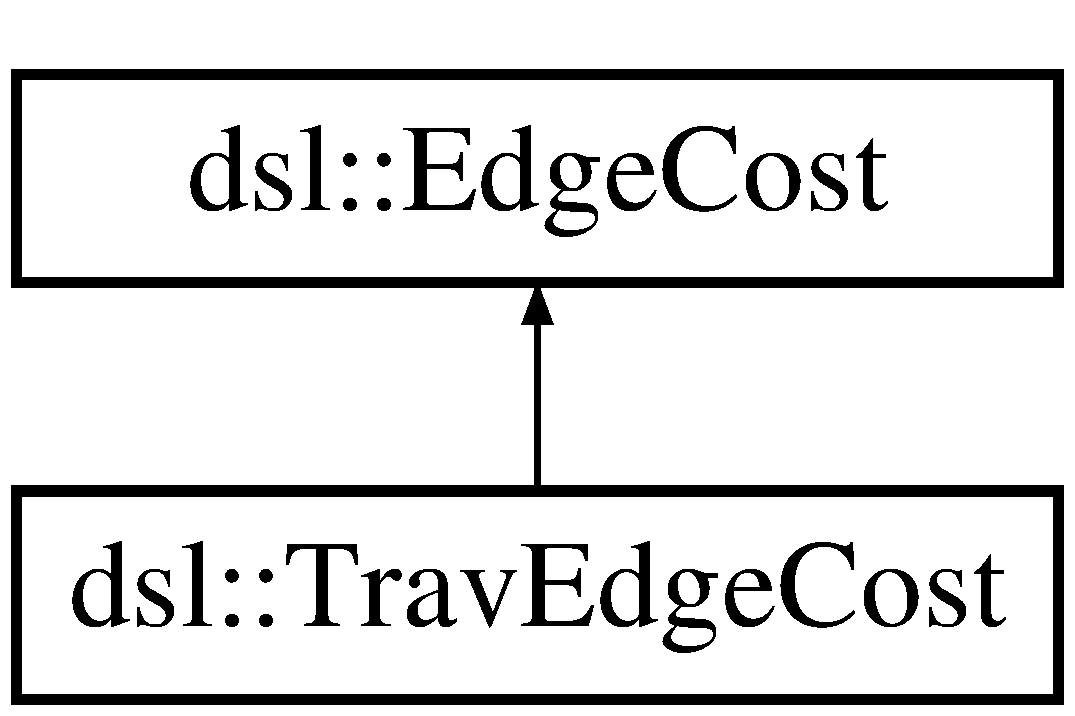
\includegraphics[height=2.000000cm]{classdsl_1_1TravEdgeCost}
\end{center}
\end{figure}
\subsection*{\-Public \-Member \-Functions}
\begin{DoxyCompactItemize}
\item 
virtual double {\bf \-Calc\-Edge\-Cost} (double v1cost, double v2cost, double elength)
\end{DoxyCompactItemize}


\subsection{\-Member \-Function \-Documentation}
\index{dsl\-::\-Trav\-Edge\-Cost@{dsl\-::\-Trav\-Edge\-Cost}!\-Calc\-Edge\-Cost@{\-Calc\-Edge\-Cost}}
\index{\-Calc\-Edge\-Cost@{\-Calc\-Edge\-Cost}!dsl::TravEdgeCost@{dsl\-::\-Trav\-Edge\-Cost}}
\subsubsection[{\-Calc\-Edge\-Cost}]{\setlength{\rightskip}{0pt plus 5cm}double {\bf \-Trav\-Edge\-Cost\-::\-Calc\-Edge\-Cost} (
\begin{DoxyParamCaption}
\item[{double}]{v1cost, }
\item[{double}]{v2cost, }
\item[{double}]{elength}
\end{DoxyParamCaption}
)\hspace{0.3cm}{\ttfamily  [virtual]}}\label{classdsl_1_1TravEdgeCost_a76e9ac094eeee2aba70d8cb89b27b2d8}
\-Calculates the cost (usually a height) gradient between two vertices. param v1cost cost of \char`\"{}from\char`\"{} vertex param v2cost cost of \char`\"{}to\char`\"{} vertex param ecost cost of edge 

\-Implements {\bf dsl\-::\-Edge\-Cost} \doxyref{}{p.}{classdsl_1_1EdgeCost_ae09d4d844afd0dda495013c4279ced33}.



\-The documentation for this class was generated from the following files\-:\begin{DoxyCompactItemize}
\item 
/home/matt/dsl/lib/{\bf travedgecost.\-h}\item 
/home/matt/dsl/lib/{\bf travedgecost.\-cc}\end{DoxyCompactItemize}

\section{dsl\-:\-:\-Vertex \-Class \-Reference}
\label{classdsl_1_1Vertex}\index{dsl\-::\-Vertex@{dsl\-::\-Vertex}}


{\ttfamily \#include $<$vertex.\-h$>$}

\subsection*{\-Public \-Member \-Functions}
\begin{DoxyCompactItemize}
\item 
{\bf \-Vertex} (void $\ast${\bf data}=0)
\item 
virtual {\bf $\sim$\-Vertex} ()
\item 
void {\bf \-Reset} ()
\item 
{\bf \-Edge} $\ast$ {\bf \-Find} (const {\bf \-Vertex} \&v, bool {\bf in}) const 
\end{DoxyCompactItemize}
\subsection*{\-Public \-Attributes}
\begin{DoxyCompactItemize}
\item 
int {\bf id}
\begin{DoxyCompactList}\small\item\em vertex id (set internally) \end{DoxyCompactList}\item 
void $\ast$ {\bf data}
\begin{DoxyCompactList}\small\item\em application data (optional) \end{DoxyCompactList}\item 
std\-::map$<$ int, {\bf \-Edge} $\ast$ $>$ {\bf in}
\begin{DoxyCompactList}\small\item\em map of incoming edges \end{DoxyCompactList}\item 
std\-::map$<$ int, {\bf \-Edge} $\ast$ $>$ {\bf out}
\begin{DoxyCompactList}\small\item\em map of outgoing edges \end{DoxyCompactList}\item 
{\bf \-Vertex} $\ast$ {\bf next}
\begin{DoxyCompactList}\small\item\em next state in a path (used for tracing paths) \end{DoxyCompactList}\item 
{\bf \-Vertex} $\ast$ {\bf prev}
\begin{DoxyCompactList}\small\item\em previous state in a path (used for tracing paths) \end{DoxyCompactList}\item 
double {\bf rhs}
\begin{DoxyCompactList}\small\item\em dsl g heuristic values (used internally) \end{DoxyCompactList}\item 
double {\bf g}
\begin{DoxyCompactList}\small\item\em dsl rhs heuristic values (used internally) \end{DoxyCompactList}\end{DoxyCompactItemize}
\subsection*{\-Protected \-Attributes}
\begin{DoxyCompactItemize}
\item 
int {\bf t}
\begin{DoxyCompactList}\small\item\em label (one of \-N\-E\-W,\-O\-P\-E\-N,\-C\-L\-O\-S\-E\-D) \end{DoxyCompactList}\item 
fibnode\-\_\-t {\bf open\-List\-Node}
\begin{DoxyCompactList}\small\item\em heap node associated to this vertex \end{DoxyCompactList}\item 
double {\bf key} [2]
\begin{DoxyCompactList}\small\item\em heap key \end{DoxyCompactList}\end{DoxyCompactItemize}
\subsection*{\-Static \-Protected \-Attributes}
\begin{DoxyCompactItemize}
\item 
static const int {\bf \-N\-E\-W} = 0
\begin{DoxyCompactList}\small\item\em open list label \-N\-E\-W \end{DoxyCompactList}\item 
static const int {\bf \-O\-P\-E\-N} = 1
\begin{DoxyCompactList}\small\item\em open list label \-O\-P\-E\-N \end{DoxyCompactList}\item 
static const int {\bf \-C\-L\-O\-S\-E\-D} = 2
\begin{DoxyCompactList}\small\item\em open list label \-C\-L\-O\-S\-E\-D \end{DoxyCompactList}\end{DoxyCompactItemize}
\subsection*{\-Friends}
\begin{DoxyCompactItemize}
\item 
class {\bf \-Graph}
\item 
class {\bf \-Search}
\item 
std\-::ostream \& {\bf operator$<$$<$} (std\-::ostream \&os, const {\bf \-Vertex} \&v)
\item 
std\-::istream \& {\bf operator$>$$>$} (std\-::istream \&is, {\bf \-Vertex} \&v)
\end{DoxyCompactItemize}


\subsection{\-Detailed \-Description}
\-Generic graph vertex containing a list of incoming and outgoing edges as well as information used for graph search algorithms. \-Specific implementations can either extend this class with extra functionality or simply pass a pointer to additional application data.

\-Marin \-Kobilarov -\/-\/ \-Copyright (\-C) 2004 

\subsection{\-Constructor \& \-Destructor \-Documentation}
\index{dsl\-::\-Vertex@{dsl\-::\-Vertex}!\-Vertex@{\-Vertex}}
\index{\-Vertex@{\-Vertex}!dsl::Vertex@{dsl\-::\-Vertex}}
\subsubsection[{\-Vertex}]{\setlength{\rightskip}{0pt plus 5cm}{\bf \-Vertex\-::\-Vertex} (
\begin{DoxyParamCaption}
\item[{void $\ast$}]{data = {\ttfamily 0}}
\end{DoxyParamCaption}
)}\label{classdsl_1_1Vertex_aadea5c14ccf996def2282684158ab1f0}
\-Initialize the vertex with an optional pointer to user data 
\begin{DoxyParams}{\-Parameters}
{\em data} & data \\
\hline
\end{DoxyParams}


\-References \-Reset().

\index{dsl\-::\-Vertex@{dsl\-::\-Vertex}!$\sim$\-Vertex@{$\sim$\-Vertex}}
\index{$\sim$\-Vertex@{$\sim$\-Vertex}!dsl::Vertex@{dsl\-::\-Vertex}}
\subsubsection[{$\sim$\-Vertex}]{\setlength{\rightskip}{0pt plus 5cm}{\bf \-Vertex\-::$\sim$\-Vertex} (
\begin{DoxyParamCaption}
{}
\end{DoxyParamCaption}
)\hspace{0.3cm}{\ttfamily  [virtual]}}\label{classdsl_1_1Vertex_ad7a0ce588b7f688dc4488a0f567d9155}


\-References in, and out.



\subsection{\-Member \-Function \-Documentation}
\index{dsl\-::\-Vertex@{dsl\-::\-Vertex}!\-Find@{\-Find}}
\index{\-Find@{\-Find}!dsl::Vertex@{dsl\-::\-Vertex}}
\subsubsection[{\-Find}]{\setlength{\rightskip}{0pt plus 5cm}{\bf \-Edge} $\ast$ {\bf \-Vertex\-::\-Find} (
\begin{DoxyParamCaption}
\item[{const {\bf \-Vertex} \&}]{v, }
\item[{bool}]{in}
\end{DoxyParamCaption}
) const}\label{classdsl_1_1Vertex_a5aa722d8a1a62d8fcf6075e9c433be4b}
\-Finds an edge that connects this vertex with a given vertex v 
\begin{DoxyParams}{\-Parameters}
{\em v} & vertex v \\
\hline
{\em in} & whether to look among incoming or outgoing edges \\
\hline
\end{DoxyParams}
\begin{DoxyReturn}{\-Returns}
the edge or 0 if none 
\end{DoxyReturn}


\-References dsl\-::\-Edge\-::from, out, and dsl\-::\-Edge\-::to.

\index{dsl\-::\-Vertex@{dsl\-::\-Vertex}!\-Reset@{\-Reset}}
\index{\-Reset@{\-Reset}!dsl::Vertex@{dsl\-::\-Vertex}}
\subsubsection[{\-Reset}]{\setlength{\rightskip}{0pt plus 5cm}void {\bf \-Vertex\-::\-Reset} (
\begin{DoxyParamCaption}
{}
\end{DoxyParamCaption}
)}\label{classdsl_1_1Vertex_a9f75c0a26a8f598a0071a86acd2b862a}
\-Reset to initial conditions (only the id is kept) 

\-References g, \-I\-N\-F, key, \-N\-E\-W, next, open\-List\-Node, prev, rhs, and t.



\-Referenced by \-Vertex().



\subsection{\-Friends \-And \-Related \-Function \-Documentation}
\index{dsl\-::\-Vertex@{dsl\-::\-Vertex}!\-Graph@{\-Graph}}
\index{\-Graph@{\-Graph}!dsl::Vertex@{dsl\-::\-Vertex}}
\subsubsection[{\-Graph}]{\setlength{\rightskip}{0pt plus 5cm}friend class {\bf \-Graph}\hspace{0.3cm}{\ttfamily  [friend]}}\label{classdsl_1_1Vertex_afab89afd724f1b07b1aaad6bdc61c47a}
\index{dsl\-::\-Vertex@{dsl\-::\-Vertex}!operator$<$$<$@{operator$<$$<$}}
\index{operator$<$$<$@{operator$<$$<$}!dsl::Vertex@{dsl\-::\-Vertex}}
\subsubsection[{operator$<$$<$}]{\setlength{\rightskip}{0pt plus 5cm}std\-::ostream\& operator$<$$<$ (
\begin{DoxyParamCaption}
\item[{std\-::ostream \&}]{os, }
\item[{const {\bf \-Vertex} \&}]{v}
\end{DoxyParamCaption}
)\hspace{0.3cm}{\ttfamily  [friend]}}\label{classdsl_1_1Vertex_aa80cb53b0a61b605b5e10d5b3fe9d505}
\-Output the vertex to a stream 
\begin{DoxyParams}{\-Parameters}
{\em os} & output stream \\
\hline
{\em v} & vertex \\
\hline
\end{DoxyParams}
\begin{DoxyReturn}{\-Returns}
the output stream 
\end{DoxyReturn}
\index{dsl\-::\-Vertex@{dsl\-::\-Vertex}!operator$>$$>$@{operator$>$$>$}}
\index{operator$>$$>$@{operator$>$$>$}!dsl::Vertex@{dsl\-::\-Vertex}}
\subsubsection[{operator$>$$>$}]{\setlength{\rightskip}{0pt plus 5cm}std\-::istream\& operator$>$$>$ (
\begin{DoxyParamCaption}
\item[{std\-::istream \&}]{is, }
\item[{{\bf \-Vertex} \&}]{v}
\end{DoxyParamCaption}
)\hspace{0.3cm}{\ttfamily  [friend]}}\label{classdsl_1_1Vertex_ad0a68acc39e3ef903add7e66757cf158}
\-Input the vertex from a stream 
\begin{DoxyParams}{\-Parameters}
{\em is} & input stream \\
\hline
{\em v} & vertex \\
\hline
\end{DoxyParams}
\begin{DoxyReturn}{\-Returns}
the input stream 
\end{DoxyReturn}
\index{dsl\-::\-Vertex@{dsl\-::\-Vertex}!\-Search@{\-Search}}
\index{\-Search@{\-Search}!dsl::Vertex@{dsl\-::\-Vertex}}
\subsubsection[{\-Search}]{\setlength{\rightskip}{0pt plus 5cm}friend class {\bf \-Search}\hspace{0.3cm}{\ttfamily  [friend]}}\label{classdsl_1_1Vertex_aea88561fddd2e924cebf793f0cfdc8b6}


\subsection{\-Member \-Data \-Documentation}
\index{dsl\-::\-Vertex@{dsl\-::\-Vertex}!\-C\-L\-O\-S\-E\-D@{\-C\-L\-O\-S\-E\-D}}
\index{\-C\-L\-O\-S\-E\-D@{\-C\-L\-O\-S\-E\-D}!dsl::Vertex@{dsl\-::\-Vertex}}
\subsubsection[{\-C\-L\-O\-S\-E\-D}]{\setlength{\rightskip}{0pt plus 5cm}const int {\bf dsl\-::\-Vertex\-::\-C\-L\-O\-S\-E\-D} = 2\hspace{0.3cm}{\ttfamily  [static, protected]}}\label{classdsl_1_1Vertex_a6f1927e13f5c9c52fe241d379790ecc4}


open list label \-C\-L\-O\-S\-E\-D 



\-Referenced by dsl\-::\-Search\-::\-Remove().

\index{dsl\-::\-Vertex@{dsl\-::\-Vertex}!data@{data}}
\index{data@{data}!dsl::Vertex@{dsl\-::\-Vertex}}
\subsubsection[{data}]{\setlength{\rightskip}{0pt plus 5cm}void$\ast$ {\bf dsl\-::\-Vertex\-::data}}\label{classdsl_1_1Vertex_a2c6f027591db54c5fbf5e50e27def3a0}


application data (optional) 



\-Referenced by dsl\-::\-Grid\-Cost\-::\-Heur(), dsl\-::\-Grid\-Cost3\-D\-::\-Heur(), dsl\-::\-Grid\-Search\-::\-Plan(), dsl\-::\-Grid\-Search3\-D\-::\-Plan(), dsl\-::\-Grid\-Cost\-::\-Real(), dsl\-::\-Grid\-Cost3\-D\-::\-Real(), dsl\-::\-Grid\-Search\-::$\sim$\-Grid\-Search(), and dsl\-::\-Grid\-Search3\-D\-::$\sim$\-Grid\-Search3\-D().

\index{dsl\-::\-Vertex@{dsl\-::\-Vertex}!g@{g}}
\index{g@{g}!dsl::Vertex@{dsl\-::\-Vertex}}
\subsubsection[{g}]{\setlength{\rightskip}{0pt plus 5cm}double {\bf dsl\-::\-Vertex\-::g}}\label{classdsl_1_1Vertex_a1792e5abf07174d4e24e5dd3d3fb6e12}


dsl rhs heuristic values (used internally) 



\-Referenced by dsl\-::\-Search\-::\-Calculate\-Ext\-Key(), dsl\-::\-Search\-::\-Compute\-Shortest\-Path(), dsl\-::\-Search\-::\-Min\-Succ(), dsl\-::operator$<$$<$(), dsl\-::\-Search\-::\-Plan(), dsl\-::\-Graph\-::\-Remove\-Edge(), \-Reset(), and dsl\-::\-Search\-::\-Update\-Vertex().

\index{dsl\-::\-Vertex@{dsl\-::\-Vertex}!id@{id}}
\index{id@{id}!dsl::Vertex@{dsl\-::\-Vertex}}
\subsubsection[{id}]{\setlength{\rightskip}{0pt plus 5cm}int {\bf dsl\-::\-Vertex\-::id}}\label{classdsl_1_1Vertex_ade0c7c448fddd603cdeb8d1775f3ae7a}


vertex id (set internally) 



\-Referenced by dsl\-::\-Graph\-::\-Add\-Vertex(), dsl\-::\-Graph\-::\-Exists(), dsl\-::operator$<$$<$(), and dsl\-::\-Graph\-::\-Remove\-Vertex().

\index{dsl\-::\-Vertex@{dsl\-::\-Vertex}!in@{in}}
\index{in@{in}!dsl::Vertex@{dsl\-::\-Vertex}}
\subsubsection[{in}]{\setlength{\rightskip}{0pt plus 5cm}std\-::map$<$int, {\bf \-Edge}$\ast$$>$ {\bf dsl\-::\-Vertex\-::in}}\label{classdsl_1_1Vertex_a0366cdb27e1674f10b033c5cad9cfe71}


map of incoming edges 



\-Referenced by dsl\-::\-Graph\-::\-Add\-Edge(), dsl\-::\-Search\-::\-Compute\-Shortest\-Path(), dsl\-::operator$<$$<$(), dsl\-::\-Search\-::\-Plan(), dsl\-::\-Graph\-::\-Remove\-Edge(), dsl\-::\-Graph\-::\-Remove\-Vertex(), dsl\-::\-Grid\-Search\-::\-Set\-Cost(), dsl\-::\-Grid\-Search3\-D\-::\-Set\-Cost(), and $\sim$\-Vertex().

\index{dsl\-::\-Vertex@{dsl\-::\-Vertex}!key@{key}}
\index{key@{key}!dsl::Vertex@{dsl\-::\-Vertex}}
\subsubsection[{key}]{\setlength{\rightskip}{0pt plus 5cm}double {\bf dsl\-::\-Vertex\-::key}[2]\hspace{0.3cm}{\ttfamily  [protected]}}\label{classdsl_1_1Vertex_a0ada3f69f585f98e0e3e4a078c979eac}


heap key 



\-Referenced by dsl\-::\-Search\-::\-Calculate\-Key(), dsl\-::\-Search\-::\-Compute\-Shortest\-Path(), dsl\-::\-Search\-::\-Insert(), dsl\-::operator$<$$<$(), \-Reset(), dsl\-::\-Search\-::\-Set\-Goal(), dsl\-::\-Search\-::\-Top\-Key(), and dsl\-::\-Search\-::\-Update().

\index{dsl\-::\-Vertex@{dsl\-::\-Vertex}!\-N\-E\-W@{\-N\-E\-W}}
\index{\-N\-E\-W@{\-N\-E\-W}!dsl::Vertex@{dsl\-::\-Vertex}}
\subsubsection[{\-N\-E\-W}]{\setlength{\rightskip}{0pt plus 5cm}const int {\bf dsl\-::\-Vertex\-::\-N\-E\-W} = 0\hspace{0.3cm}{\ttfamily  [static, protected]}}\label{classdsl_1_1Vertex_a44275282e5f7b0be43bcc153621f1f6d}


open list label \-N\-E\-W 



\-Referenced by \-Reset().

\index{dsl\-::\-Vertex@{dsl\-::\-Vertex}!next@{next}}
\index{next@{next}!dsl::Vertex@{dsl\-::\-Vertex}}
\subsubsection[{next}]{\setlength{\rightskip}{0pt plus 5cm}{\bf \-Vertex}$\ast$ {\bf dsl\-::\-Vertex\-::next}}\label{classdsl_1_1Vertex_a8d1304ddb4aac965291b30f25d8a24a4}


next state in a path (used for tracing paths) 



\-Referenced by dsl\-::operator$<$$<$(), dsl\-::\-Grid\-Search\-::\-Plan(), dsl\-::\-Search\-::\-Plan(), dsl\-::\-Grid\-Search3\-D\-::\-Plan(), and \-Reset().

\index{dsl\-::\-Vertex@{dsl\-::\-Vertex}!\-O\-P\-E\-N@{\-O\-P\-E\-N}}
\index{\-O\-P\-E\-N@{\-O\-P\-E\-N}!dsl::Vertex@{dsl\-::\-Vertex}}
\subsubsection[{\-O\-P\-E\-N}]{\setlength{\rightskip}{0pt plus 5cm}const int {\bf dsl\-::\-Vertex\-::\-O\-P\-E\-N} = 1\hspace{0.3cm}{\ttfamily  [static, protected]}}\label{classdsl_1_1Vertex_a76be5b53d16bd35ef36992609b05b5e1}


open list label \-O\-P\-E\-N 



\-Referenced by dsl\-::\-Search\-::\-Insert\-Ext(), dsl\-::\-Search\-::\-Update(), and dsl\-::\-Search\-::\-Update\-Vertex().

\index{dsl\-::\-Vertex@{dsl\-::\-Vertex}!open\-List\-Node@{open\-List\-Node}}
\index{open\-List\-Node@{open\-List\-Node}!dsl::Vertex@{dsl\-::\-Vertex}}
\subsubsection[{open\-List\-Node}]{\setlength{\rightskip}{0pt plus 5cm}fibnode\-\_\-t {\bf dsl\-::\-Vertex\-::open\-List\-Node}\hspace{0.3cm}{\ttfamily  [protected]}}\label{classdsl_1_1Vertex_a407f820d27408e3716ca42347d3a432f}


heap node associated to this vertex 



\-Referenced by dsl\-::\-Search\-::\-Insert\-Ext(), dsl\-::operator$<$$<$(), dsl\-::\-Search\-::\-Remove(), dsl\-::\-Graph\-::\-Remove\-Edge(), \-Reset(), and dsl\-::\-Search\-::\-Update().

\index{dsl\-::\-Vertex@{dsl\-::\-Vertex}!out@{out}}
\index{out@{out}!dsl::Vertex@{dsl\-::\-Vertex}}
\subsubsection[{out}]{\setlength{\rightskip}{0pt plus 5cm}std\-::map$<$int, {\bf \-Edge}$\ast$$>$ {\bf dsl\-::\-Vertex\-::out}}\label{classdsl_1_1Vertex_a8eece6b931c93f951100d2ab988c8666}


map of outgoing edges 



\-Referenced by dsl\-::\-Graph\-::\-Add\-Edge(), \-Find(), dsl\-::\-Search\-::\-Min\-Succ(), dsl\-::operator$<$$<$(), dsl\-::\-Search\-::\-Plan(), dsl\-::\-Graph\-::\-Remove\-Edge(), dsl\-::\-Graph\-::\-Remove\-Vertex(), dsl\-::\-Grid\-Search\-::\-Set\-Cost(), dsl\-::\-Grid\-Search3\-D\-::\-Set\-Cost(), and $\sim$\-Vertex().

\index{dsl\-::\-Vertex@{dsl\-::\-Vertex}!prev@{prev}}
\index{prev@{prev}!dsl::Vertex@{dsl\-::\-Vertex}}
\subsubsection[{prev}]{\setlength{\rightskip}{0pt plus 5cm}{\bf \-Vertex}$\ast$ {\bf dsl\-::\-Vertex\-::prev}}\label{classdsl_1_1Vertex_a872a93b3aff52d54e65d2346f95f46e3}


previous state in a path (used for tracing paths) 



\-Referenced by dsl\-::\-Search\-::\-Plan(), and \-Reset().

\index{dsl\-::\-Vertex@{dsl\-::\-Vertex}!rhs@{rhs}}
\index{rhs@{rhs}!dsl::Vertex@{dsl\-::\-Vertex}}
\subsubsection[{rhs}]{\setlength{\rightskip}{0pt plus 5cm}double {\bf dsl\-::\-Vertex\-::rhs}}\label{classdsl_1_1Vertex_ad9a72f64c36b5f7fa4f3521d3012a2ff}


dsl g heuristic values (used internally) 



\-Referenced by dsl\-::\-Search\-::\-Calculate\-Ext\-Key(), dsl\-::\-Search\-::\-Compute\-Shortest\-Path(), dsl\-::operator$<$$<$(), dsl\-::\-Search\-::\-Plan(), dsl\-::\-Graph\-::\-Remove\-Edge(), \-Reset(), dsl\-::\-Search\-::\-Set\-Goal(), and dsl\-::\-Search\-::\-Update\-Vertex().

\index{dsl\-::\-Vertex@{dsl\-::\-Vertex}!t@{t}}
\index{t@{t}!dsl::Vertex@{dsl\-::\-Vertex}}
\subsubsection[{t}]{\setlength{\rightskip}{0pt plus 5cm}int {\bf dsl\-::\-Vertex\-::t}\hspace{0.3cm}{\ttfamily  [protected]}}\label{classdsl_1_1Vertex_a37774ca86c886bfd93a2b5e1f22328b5}


label (one of \-N\-E\-W,\-O\-P\-E\-N,\-C\-L\-O\-S\-E\-D) 



\-Referenced by dsl\-::\-Search\-::\-Insert\-Ext(), dsl\-::operator$<$$<$(), dsl\-::\-Search\-::\-Remove(), \-Reset(), dsl\-::\-Search\-::\-Update(), and dsl\-::\-Search\-::\-Update\-Vertex().



\-The documentation for this class was generated from the following files\-:\begin{DoxyCompactItemize}
\item 
/home/matt/dsl/lib/{\bf vertex.\-h}\item 
/home/matt/dsl/lib/{\bf vertex.\-cc}\end{DoxyCompactItemize}

\chapter{\-File \-Documentation}
\section{/home/matt/dsl/bin/test.cc \-File \-Reference}
\label{test_8cc}\index{/home/matt/dsl/bin/test.\-cc@{/home/matt/dsl/bin/test.\-cc}}
{\ttfamily \#include $<$stdio.\-h$>$}\*
{\ttfamily \#include $<$assert.\-h$>$}\*
{\ttfamily \#include $<$math.\-h$>$}\*
{\ttfamily \#include $<$sys/time.\-h$>$}\*
{\ttfamily \#include $<$stdlib.\-h$>$}\*
{\ttfamily \#include $<$string.\-h$>$}\*
{\ttfamily \#include \char`\"{}gridsearch.\-h\char`\"{}}\*
\subsection*{\-Functions}
\begin{DoxyCompactItemize}
\item 
void {\bf save\-\_\-map} (const char $\ast$map, int width, int height, const char $\ast$filename)
\item 
char $\ast$ {\bf load\-\_\-map} (int $\ast$width, int $\ast$height, const char $\ast$filename)
\item 
void {\bf timer\-\_\-start} (struct timeval $\ast$time)
\item 
long {\bf timer\-\_\-us} (struct timeval $\ast$time)
\item 
int {\bf main} (int argc, char $\ast$$\ast$argv)
\end{DoxyCompactItemize}


\subsection{\-Function \-Documentation}
\index{test.\-cc@{test.\-cc}!load\-\_\-map@{load\-\_\-map}}
\index{load\-\_\-map@{load\-\_\-map}!test.cc@{test.\-cc}}
\subsubsection[{load\-\_\-map}]{\setlength{\rightskip}{0pt plus 5cm}char$\ast$ {\bf load\-\_\-map} (
\begin{DoxyParamCaption}
\item[{int $\ast$}]{width, }
\item[{int $\ast$}]{height, }
\item[{const char $\ast$}]{filename}
\end{DoxyParamCaption}
)}\label{test_8cc_a358a7f4a8709529d700da886d011fb71}


\-Referenced by main().

\index{test.\-cc@{test.\-cc}!main@{main}}
\index{main@{main}!test.cc@{test.\-cc}}
\subsubsection[{main}]{\setlength{\rightskip}{0pt plus 5cm}int {\bf main} (
\begin{DoxyParamCaption}
\item[{int}]{argc, }
\item[{char $\ast$$\ast$}]{argv}
\end{DoxyParamCaption}
)}\label{test_8cc_a3c04138a5bfe5d72780bb7e82a18e627}


\-References dsl\-::\-Grid\-Path\-::count, dsl\-::\-Grid\-Path\-::len, load\-\_\-map(), dsl\-::\-Grid\-Search\-::\-Opt\-Path(), dsl\-::\-Grid\-Search\-::\-Plan(), dsl\-::\-Grid\-Path\-::pos, dsl\-::\-Grid\-Search\-::\-Remove\-Vertex(), save\-\_\-map(), dsl\-::\-Grid\-Search\-::\-Set\-Cost(), dsl\-::\-Grid\-Search\-::\-Set\-Goal(), dsl\-::\-Grid\-Search\-::\-Set\-Start(), timer\-\_\-start(), and timer\-\_\-us().

\index{test.\-cc@{test.\-cc}!save\-\_\-map@{save\-\_\-map}}
\index{save\-\_\-map@{save\-\_\-map}!test.cc@{test.\-cc}}
\subsubsection[{save\-\_\-map}]{\setlength{\rightskip}{0pt plus 5cm}void {\bf save\-\_\-map} (
\begin{DoxyParamCaption}
\item[{const char $\ast$}]{map, }
\item[{int}]{width, }
\item[{int}]{height, }
\item[{const char $\ast$}]{filename}
\end{DoxyParamCaption}
)}\label{test_8cc_afe51d8578a491f419faac8d7f72dc76c}


\-Referenced by main().

\index{test.\-cc@{test.\-cc}!timer\-\_\-start@{timer\-\_\-start}}
\index{timer\-\_\-start@{timer\-\_\-start}!test.cc@{test.\-cc}}
\subsubsection[{timer\-\_\-start}]{\setlength{\rightskip}{0pt plus 5cm}void {\bf timer\-\_\-start} (
\begin{DoxyParamCaption}
\item[{struct timeval $\ast$}]{time}
\end{DoxyParamCaption}
)}\label{test_8cc_a95579c03aab7cc44004af8cdd5f1ccd0}


\-Referenced by main().

\index{test.\-cc@{test.\-cc}!timer\-\_\-us@{timer\-\_\-us}}
\index{timer\-\_\-us@{timer\-\_\-us}!test.cc@{test.\-cc}}
\subsubsection[{timer\-\_\-us}]{\setlength{\rightskip}{0pt plus 5cm}long {\bf timer\-\_\-us} (
\begin{DoxyParamCaption}
\item[{struct timeval $\ast$}]{time}
\end{DoxyParamCaption}
)}\label{test_8cc_ae8df24716ff9bc0ec9bde1931f2c01d4}


\-Referenced by main().


\section{build/\-C\-Make\-Files/2.8.12.2/\-Compiler\-Id\-C/\-C\-Make\-C\-Compiler\-Id.c File Reference}
\label{CMakeCCompilerId_8c}\index{build/\-C\-Make\-Files/2.\-8.\-12.\-2/\-Compiler\-Id\-C/\-C\-Make\-C\-Compiler\-Id.\-c@{build/\-C\-Make\-Files/2.\-8.\-12.\-2/\-Compiler\-Id\-C/\-C\-Make\-C\-Compiler\-Id.\-c}}
\subsection*{Macros}
\begin{DoxyCompactItemize}
\item 
\#define {\bf C\-O\-M\-P\-I\-L\-E\-R\-\_\-\-I\-D}~\char`\"{}\char`\"{}
\item 
\#define {\bf P\-L\-A\-T\-F\-O\-R\-M\-\_\-\-I\-D}~\char`\"{}\char`\"{}
\item 
\#define {\bf A\-R\-C\-H\-I\-T\-E\-C\-T\-U\-R\-E\-\_\-\-I\-D}~\char`\"{}\char`\"{}
\item 
\#define {\bf D\-E\-C}(n)
\item 
\#define {\bf H\-E\-X}(n)
\end{DoxyCompactItemize}
\subsection*{Functions}
\begin{DoxyCompactItemize}
\item 
int {\bf main} (int argc, char $\ast$argv[$\,$])
\end{DoxyCompactItemize}
\subsection*{Variables}
\begin{DoxyCompactItemize}
\item 
char const $\ast$ {\bf info\-\_\-compiler} = \char`\"{}I\-N\-F\-O\char`\"{} \char`\"{}\-:\char`\"{} \char`\"{}compiler[\char`\"{} C\-O\-M\-P\-I\-L\-E\-R\-\_\-\-I\-D \char`\"{}]\char`\"{}
\item 
char const $\ast$ {\bf info\-\_\-platform} = \char`\"{}I\-N\-F\-O\char`\"{} \char`\"{}\-:\char`\"{} \char`\"{}platform[\char`\"{} P\-L\-A\-T\-F\-O\-R\-M\-\_\-\-I\-D \char`\"{}]\char`\"{}
\item 
char const $\ast$ {\bf info\-\_\-arch} = \char`\"{}I\-N\-F\-O\char`\"{} \char`\"{}\-:\char`\"{} \char`\"{}arch[\char`\"{} A\-R\-C\-H\-I\-T\-E\-C\-T\-U\-R\-E\-\_\-\-I\-D \char`\"{}]\char`\"{}
\end{DoxyCompactItemize}


\subsection{Macro Definition Documentation}
\index{C\-Make\-C\-Compiler\-Id.\-c@{C\-Make\-C\-Compiler\-Id.\-c}!A\-R\-C\-H\-I\-T\-E\-C\-T\-U\-R\-E\-\_\-\-I\-D@{A\-R\-C\-H\-I\-T\-E\-C\-T\-U\-R\-E\-\_\-\-I\-D}}
\index{A\-R\-C\-H\-I\-T\-E\-C\-T\-U\-R\-E\-\_\-\-I\-D@{A\-R\-C\-H\-I\-T\-E\-C\-T\-U\-R\-E\-\_\-\-I\-D}!CMakeCCompilerId.c@{C\-Make\-C\-Compiler\-Id.\-c}}
\subsubsection[{A\-R\-C\-H\-I\-T\-E\-C\-T\-U\-R\-E\-\_\-\-I\-D}]{\setlength{\rightskip}{0pt plus 5cm}\#define A\-R\-C\-H\-I\-T\-E\-C\-T\-U\-R\-E\-\_\-\-I\-D~\char`\"{}\char`\"{}}\label{CMakeCCompilerId_8c_aba35d0d200deaeb06aee95ca297acb28}
\index{C\-Make\-C\-Compiler\-Id.\-c@{C\-Make\-C\-Compiler\-Id.\-c}!C\-O\-M\-P\-I\-L\-E\-R\-\_\-\-I\-D@{C\-O\-M\-P\-I\-L\-E\-R\-\_\-\-I\-D}}
\index{C\-O\-M\-P\-I\-L\-E\-R\-\_\-\-I\-D@{C\-O\-M\-P\-I\-L\-E\-R\-\_\-\-I\-D}!CMakeCCompilerId.c@{C\-Make\-C\-Compiler\-Id.\-c}}
\subsubsection[{C\-O\-M\-P\-I\-L\-E\-R\-\_\-\-I\-D}]{\setlength{\rightskip}{0pt plus 5cm}\#define C\-O\-M\-P\-I\-L\-E\-R\-\_\-\-I\-D~\char`\"{}\char`\"{}}\label{CMakeCCompilerId_8c_a81dee0709ded976b2e0319239f72d174}
\index{C\-Make\-C\-Compiler\-Id.\-c@{C\-Make\-C\-Compiler\-Id.\-c}!D\-E\-C@{D\-E\-C}}
\index{D\-E\-C@{D\-E\-C}!CMakeCCompilerId.c@{C\-Make\-C\-Compiler\-Id.\-c}}
\subsubsection[{D\-E\-C}]{\setlength{\rightskip}{0pt plus 5cm}\#define D\-E\-C(
\begin{DoxyParamCaption}
\item[{}]{n}
\end{DoxyParamCaption}
)}\label{CMakeCCompilerId_8c_ad1280362da42492bbc11aa78cbf776ad}
{\bfseries Value\-:}
\begin{DoxyCode}
(\textcolor{charliteral}{'0'} + (((n) / 10000000)%10)), \(\backslash\)
  (\textcolor{charliteral}{'0'} + (((n) / 1000000)%10)),  \(\backslash\)
  (\textcolor{charliteral}{'0'} + (((n) / 100000)%10)),   \(\backslash\)
  (\textcolor{charliteral}{'0'} + (((n) / 10000)%10)),    \(\backslash\)
  (\textcolor{charliteral}{'0'} + (((n) / 1000)%10)),     \(\backslash\)
  (\textcolor{charliteral}{'0'} + (((n) / 100)%10)),      \(\backslash\)
  (\textcolor{charliteral}{'0'} + (((n) / 10)%10)),       \(\backslash\)
  (\textcolor{charliteral}{'0'} +  ((n) % 10))
\end{DoxyCode}
\index{C\-Make\-C\-Compiler\-Id.\-c@{C\-Make\-C\-Compiler\-Id.\-c}!H\-E\-X@{H\-E\-X}}
\index{H\-E\-X@{H\-E\-X}!CMakeCCompilerId.c@{C\-Make\-C\-Compiler\-Id.\-c}}
\subsubsection[{H\-E\-X}]{\setlength{\rightskip}{0pt plus 5cm}\#define H\-E\-X(
\begin{DoxyParamCaption}
\item[{}]{n}
\end{DoxyParamCaption}
)}\label{CMakeCCompilerId_8c_a46d5d95daa1bef867bd0179594310ed5}
{\bfseries Value\-:}
\begin{DoxyCode}
(\textcolor{charliteral}{'0'} + ((n)>>28 & 0xF)), \(\backslash\)
  (\textcolor{charliteral}{'0'} + ((n)>>24 & 0xF)), \(\backslash\)
  (\textcolor{charliteral}{'0'} + ((n)>>20 & 0xF)), \(\backslash\)
  (\textcolor{charliteral}{'0'} + ((n)>>16 & 0xF)), \(\backslash\)
  (\textcolor{charliteral}{'0'} + ((n)>>12 & 0xF)), \(\backslash\)
  (\textcolor{charliteral}{'0'} + ((n)>>8  & 0xF)), \(\backslash\)
  (\textcolor{charliteral}{'0'} + ((n)>>4  & 0xF)), \(\backslash\)
  (\textcolor{charliteral}{'0'} + ((n)     & 0xF))
\end{DoxyCode}
\index{C\-Make\-C\-Compiler\-Id.\-c@{C\-Make\-C\-Compiler\-Id.\-c}!P\-L\-A\-T\-F\-O\-R\-M\-\_\-\-I\-D@{P\-L\-A\-T\-F\-O\-R\-M\-\_\-\-I\-D}}
\index{P\-L\-A\-T\-F\-O\-R\-M\-\_\-\-I\-D@{P\-L\-A\-T\-F\-O\-R\-M\-\_\-\-I\-D}!CMakeCCompilerId.c@{C\-Make\-C\-Compiler\-Id.\-c}}
\subsubsection[{P\-L\-A\-T\-F\-O\-R\-M\-\_\-\-I\-D}]{\setlength{\rightskip}{0pt plus 5cm}\#define P\-L\-A\-T\-F\-O\-R\-M\-\_\-\-I\-D~\char`\"{}\char`\"{}}\label{CMakeCCompilerId_8c_adbc5372f40838899018fadbc89bd588b}


\subsection{Function Documentation}
\index{C\-Make\-C\-Compiler\-Id.\-c@{C\-Make\-C\-Compiler\-Id.\-c}!main@{main}}
\index{main@{main}!CMakeCCompilerId.c@{C\-Make\-C\-Compiler\-Id.\-c}}
\subsubsection[{main}]{\setlength{\rightskip}{0pt plus 5cm}int main (
\begin{DoxyParamCaption}
\item[{int}]{argc, }
\item[{char $\ast$}]{argv[$\,$]}
\end{DoxyParamCaption}
)}\label{CMakeCCompilerId_8c_a0ddf1224851353fc92bfbff6f499fa97}


References info\-\_\-arch, info\-\_\-compiler, and info\-\_\-platform.



\subsection{Variable Documentation}
\index{C\-Make\-C\-Compiler\-Id.\-c@{C\-Make\-C\-Compiler\-Id.\-c}!info\-\_\-arch@{info\-\_\-arch}}
\index{info\-\_\-arch@{info\-\_\-arch}!CMakeCCompilerId.c@{C\-Make\-C\-Compiler\-Id.\-c}}
\subsubsection[{info\-\_\-arch}]{\setlength{\rightskip}{0pt plus 5cm}char const$\ast$ info\-\_\-arch = \char`\"{}I\-N\-F\-O\char`\"{} \char`\"{}\-:\char`\"{} \char`\"{}arch[\char`\"{} A\-R\-C\-H\-I\-T\-E\-C\-T\-U\-R\-E\-\_\-\-I\-D \char`\"{}]\char`\"{}}\label{CMakeCCompilerId_8c_a59647e99d304ed33b15cb284c27ed391}


Referenced by main().

\index{C\-Make\-C\-Compiler\-Id.\-c@{C\-Make\-C\-Compiler\-Id.\-c}!info\-\_\-compiler@{info\-\_\-compiler}}
\index{info\-\_\-compiler@{info\-\_\-compiler}!CMakeCCompilerId.c@{C\-Make\-C\-Compiler\-Id.\-c}}
\subsubsection[{info\-\_\-compiler}]{\setlength{\rightskip}{0pt plus 5cm}char const$\ast$ info\-\_\-compiler = \char`\"{}I\-N\-F\-O\char`\"{} \char`\"{}\-:\char`\"{} \char`\"{}compiler[\char`\"{} C\-O\-M\-P\-I\-L\-E\-R\-\_\-\-I\-D \char`\"{}]\char`\"{}}\label{CMakeCCompilerId_8c_a4b0efeb7a5d59313986b3a0390f050f6}


Referenced by main().

\index{C\-Make\-C\-Compiler\-Id.\-c@{C\-Make\-C\-Compiler\-Id.\-c}!info\-\_\-platform@{info\-\_\-platform}}
\index{info\-\_\-platform@{info\-\_\-platform}!CMakeCCompilerId.c@{C\-Make\-C\-Compiler\-Id.\-c}}
\subsubsection[{info\-\_\-platform}]{\setlength{\rightskip}{0pt plus 5cm}char const$\ast$ info\-\_\-platform = \char`\"{}I\-N\-F\-O\char`\"{} \char`\"{}\-:\char`\"{} \char`\"{}platform[\char`\"{} P\-L\-A\-T\-F\-O\-R\-M\-\_\-\-I\-D \char`\"{}]\char`\"{}}\label{CMakeCCompilerId_8c_a2321403dee54ee23f0c2fa849c60f7d4}


Referenced by main().


\section{\-C\-Make\-Files/\-Compiler\-Id\-C\-X\-X/\-C\-Make\-C\-X\-X\-Compiler\-Id.cpp \-File \-Reference}
\label{CMakeCXXCompilerId_8cpp}\index{\-C\-Make\-Files/\-Compiler\-Id\-C\-X\-X/\-C\-Make\-C\-X\-X\-Compiler\-Id.\-cpp@{\-C\-Make\-Files/\-Compiler\-Id\-C\-X\-X/\-C\-Make\-C\-X\-X\-Compiler\-Id.\-cpp}}
\subsection*{\-Defines}
\begin{DoxyCompactItemize}
\item 
\#define {\bf \-C\-O\-M\-P\-I\-L\-E\-R\-\_\-\-I\-D}~\char`\"{}\char`\"{}
\item 
\#define {\bf \-P\-L\-A\-T\-F\-O\-R\-M\-\_\-\-I\-D}~\char`\"{}\char`\"{}
\item 
\#define {\bf \-A\-R\-C\-H\-I\-T\-E\-C\-T\-U\-R\-E\-\_\-\-I\-D}~\char`\"{}\char`\"{}
\end{DoxyCompactItemize}
\subsection*{\-Functions}
\begin{DoxyCompactItemize}
\item 
int {\bf main} (int argc, char $\ast$argv[$\,$])
\end{DoxyCompactItemize}
\subsection*{\-Variables}
\begin{DoxyCompactItemize}
\item 
char const $\ast$ {\bf info\-\_\-compiler} = \char`\"{}]\char`\"{}
\item 
char const $\ast$ {\bf info\-\_\-platform} = \char`\"{}]\char`\"{}
\item 
char const $\ast$ {\bf info\-\_\-arch} = \char`\"{}]\char`\"{}
\end{DoxyCompactItemize}


\subsection{\-Define \-Documentation}
\index{\-C\-Make\-C\-X\-X\-Compiler\-Id.\-cpp@{\-C\-Make\-C\-X\-X\-Compiler\-Id.\-cpp}!\-A\-R\-C\-H\-I\-T\-E\-C\-T\-U\-R\-E\-\_\-\-I\-D@{\-A\-R\-C\-H\-I\-T\-E\-C\-T\-U\-R\-E\-\_\-\-I\-D}}
\index{\-A\-R\-C\-H\-I\-T\-E\-C\-T\-U\-R\-E\-\_\-\-I\-D@{\-A\-R\-C\-H\-I\-T\-E\-C\-T\-U\-R\-E\-\_\-\-I\-D}!CMakeCXXCompilerId.cpp@{\-C\-Make\-C\-X\-X\-Compiler\-Id.\-cpp}}
\subsubsection[{\-A\-R\-C\-H\-I\-T\-E\-C\-T\-U\-R\-E\-\_\-\-I\-D}]{\setlength{\rightskip}{0pt plus 5cm}\#define {\bf \-A\-R\-C\-H\-I\-T\-E\-C\-T\-U\-R\-E\-\_\-\-I\-D}~\char`\"{}\char`\"{}}\label{CMakeCXXCompilerId_8cpp_aba35d0d200deaeb06aee95ca297acb28}
\index{\-C\-Make\-C\-X\-X\-Compiler\-Id.\-cpp@{\-C\-Make\-C\-X\-X\-Compiler\-Id.\-cpp}!\-C\-O\-M\-P\-I\-L\-E\-R\-\_\-\-I\-D@{\-C\-O\-M\-P\-I\-L\-E\-R\-\_\-\-I\-D}}
\index{\-C\-O\-M\-P\-I\-L\-E\-R\-\_\-\-I\-D@{\-C\-O\-M\-P\-I\-L\-E\-R\-\_\-\-I\-D}!CMakeCXXCompilerId.cpp@{\-C\-Make\-C\-X\-X\-Compiler\-Id.\-cpp}}
\subsubsection[{\-C\-O\-M\-P\-I\-L\-E\-R\-\_\-\-I\-D}]{\setlength{\rightskip}{0pt plus 5cm}\#define {\bf \-C\-O\-M\-P\-I\-L\-E\-R\-\_\-\-I\-D}~\char`\"{}\char`\"{}}\label{CMakeCXXCompilerId_8cpp_a81dee0709ded976b2e0319239f72d174}
\index{\-C\-Make\-C\-X\-X\-Compiler\-Id.\-cpp@{\-C\-Make\-C\-X\-X\-Compiler\-Id.\-cpp}!\-P\-L\-A\-T\-F\-O\-R\-M\-\_\-\-I\-D@{\-P\-L\-A\-T\-F\-O\-R\-M\-\_\-\-I\-D}}
\index{\-P\-L\-A\-T\-F\-O\-R\-M\-\_\-\-I\-D@{\-P\-L\-A\-T\-F\-O\-R\-M\-\_\-\-I\-D}!CMakeCXXCompilerId.cpp@{\-C\-Make\-C\-X\-X\-Compiler\-Id.\-cpp}}
\subsubsection[{\-P\-L\-A\-T\-F\-O\-R\-M\-\_\-\-I\-D}]{\setlength{\rightskip}{0pt plus 5cm}\#define {\bf \-P\-L\-A\-T\-F\-O\-R\-M\-\_\-\-I\-D}~\char`\"{}\char`\"{}}\label{CMakeCXXCompilerId_8cpp_adbc5372f40838899018fadbc89bd588b}


\subsection{\-Function \-Documentation}
\index{\-C\-Make\-C\-X\-X\-Compiler\-Id.\-cpp@{\-C\-Make\-C\-X\-X\-Compiler\-Id.\-cpp}!main@{main}}
\index{main@{main}!CMakeCXXCompilerId.cpp@{\-C\-Make\-C\-X\-X\-Compiler\-Id.\-cpp}}
\subsubsection[{main}]{\setlength{\rightskip}{0pt plus 5cm}int {\bf main} (
\begin{DoxyParamCaption}
\item[{int}]{argc, }
\item[{char $\ast$}]{argv[$\,$]}
\end{DoxyParamCaption}
)}\label{CMakeCXXCompilerId_8cpp_a0ddf1224851353fc92bfbff6f499fa97}


\-References info\-\_\-compiler, and info\-\_\-platform.



\subsection{\-Variable \-Documentation}
\index{\-C\-Make\-C\-X\-X\-Compiler\-Id.\-cpp@{\-C\-Make\-C\-X\-X\-Compiler\-Id.\-cpp}!info\-\_\-arch@{info\-\_\-arch}}
\index{info\-\_\-arch@{info\-\_\-arch}!CMakeCXXCompilerId.cpp@{\-C\-Make\-C\-X\-X\-Compiler\-Id.\-cpp}}
\subsubsection[{info\-\_\-arch}]{\setlength{\rightskip}{0pt plus 5cm}char const$\ast$ {\bf info\-\_\-arch} = \char`\"{}]\char`\"{}}\label{CMakeCXXCompilerId_8cpp_a59647e99d304ed33b15cb284c27ed391}
\index{\-C\-Make\-C\-X\-X\-Compiler\-Id.\-cpp@{\-C\-Make\-C\-X\-X\-Compiler\-Id.\-cpp}!info\-\_\-compiler@{info\-\_\-compiler}}
\index{info\-\_\-compiler@{info\-\_\-compiler}!CMakeCXXCompilerId.cpp@{\-C\-Make\-C\-X\-X\-Compiler\-Id.\-cpp}}
\subsubsection[{info\-\_\-compiler}]{\setlength{\rightskip}{0pt plus 5cm}char const$\ast$ {\bf info\-\_\-compiler} = \char`\"{}]\char`\"{}}\label{CMakeCXXCompilerId_8cpp_a4b0efeb7a5d59313986b3a0390f050f6}
\index{\-C\-Make\-C\-X\-X\-Compiler\-Id.\-cpp@{\-C\-Make\-C\-X\-X\-Compiler\-Id.\-cpp}!info\-\_\-platform@{info\-\_\-platform}}
\index{info\-\_\-platform@{info\-\_\-platform}!CMakeCXXCompilerId.cpp@{\-C\-Make\-C\-X\-X\-Compiler\-Id.\-cpp}}
\subsubsection[{info\-\_\-platform}]{\setlength{\rightskip}{0pt plus 5cm}char const$\ast$ {\bf info\-\_\-platform} = \char`\"{}]\char`\"{}}\label{CMakeCXXCompilerId_8cpp_a2321403dee54ee23f0c2fa849c60f7d4}

\section{lib/cost.cc File Reference}
\label{cost_8cc}\index{lib/cost.\-cc@{lib/cost.\-cc}}
{\ttfamily \#include \char`\"{}cost.\-h\char`\"{}}\\*

\section{lib/cost.h File Reference}
\label{cost_8h}\index{lib/cost.\-h@{lib/cost.\-h}}
{\ttfamily \#include \char`\"{}vertex.\-h\char`\"{}}\\*
\subsection*{Classes}
\begin{DoxyCompactItemize}
\item 
class {\bf dsl\-::\-Cost}
\end{DoxyCompactItemize}
\subsection*{Namespaces}
\begin{DoxyCompactItemize}
\item 
{\bf dsl}
\end{DoxyCompactItemize}

\section{/home/matt/dsl/lib/distedgecost.cc \-File \-Reference}
\label{distedgecost_8cc}\index{/home/matt/dsl/lib/distedgecost.\-cc@{/home/matt/dsl/lib/distedgecost.\-cc}}
{\ttfamily \#include $<$assert.\-h$>$}\*
{\ttfamily \#include $<$math.\-h$>$}\*
{\ttfamily \#include $<$stdlib.\-h$>$}\*
{\ttfamily \#include $<$iostream$>$}\*
{\ttfamily \#include \char`\"{}distedgecost.\-h\char`\"{}}\*

\section{/home/matt/dsl/lib/distedgecost.h \-File \-Reference}
\label{distedgecost_8h}\index{/home/matt/dsl/lib/distedgecost.\-h@{/home/matt/dsl/lib/distedgecost.\-h}}
{\ttfamily \#include \char`\"{}edgecost.\-h\char`\"{}}\*
\subsection*{\-Classes}
\begin{DoxyCompactItemize}
\item 
class {\bf dsl\-::\-Dist\-Edge\-Cost}
\end{DoxyCompactItemize}
\subsection*{\-Namespaces}
\begin{DoxyCompactItemize}
\item 
namespace {\bf dsl}
\end{DoxyCompactItemize}

\section{lib/edge.cc File Reference}
\label{edge_8cc}\index{lib/edge.\-cc@{lib/edge.\-cc}}
{\ttfamily \#include \char`\"{}edge.\-h\char`\"{}}\\*
{\ttfamily \#include \char`\"{}vertex.\-h\char`\"{}}\\*
\subsection*{Namespaces}
\begin{DoxyCompactItemize}
\item 
{\bf dsl}
\end{DoxyCompactItemize}
\subsection*{Functions}
\begin{DoxyCompactItemize}
\item 
std\-::ostream \& {\bf dsl\-::operator$<$$<$} (std\-::ostream \&os, const {\bf Edge} \&e)
\item 
std\-::istream \& {\bf dsl\-::operator$>$$>$} (std\-::istream \&is, {\bf Edge} \&e)
\end{DoxyCompactItemize}

\section{/home/matt/dsl/lib/edge.h \-File \-Reference}
\label{edge_8h}\index{/home/matt/dsl/lib/edge.\-h@{/home/matt/dsl/lib/edge.\-h}}
{\ttfamily \#include $<$iostream$>$}\*
{\ttfamily \#include $<$iomanip$>$}\*
{\ttfamily \#include $<$stdlib.\-h$>$}\*
{\ttfamily \#include $<$string$>$}\*
\subsection*{\-Classes}
\begin{DoxyCompactItemize}
\item 
class {\bf dsl\-::\-Edge}
\end{DoxyCompactItemize}
\subsection*{\-Namespaces}
\begin{DoxyCompactItemize}
\item 
namespace {\bf dsl}
\end{DoxyCompactItemize}
\subsection*{\-Functions}
\begin{DoxyCompactItemize}
\item 
std\-::ostream \& {\bf dsl\-::operator$<$$<$} (std\-::ostream \&os, const {\bf \-Edge} \&e)
\item 
std\-::istream \& {\bf dsl\-::operator$>$$>$} (std\-::istream \&is, {\bf \-Edge} \&e)
\end{DoxyCompactItemize}

\section{/home/matt/dsl/lib/edgecost.h \-File \-Reference}
\label{edgecost_8h}\index{/home/matt/dsl/lib/edgecost.\-h@{/home/matt/dsl/lib/edgecost.\-h}}
\subsection*{\-Classes}
\begin{DoxyCompactItemize}
\item 
class {\bf dsl\-::\-Edge\-Cost}
\end{DoxyCompactItemize}
\subsection*{\-Namespaces}
\begin{DoxyCompactItemize}
\item 
namespace {\bf dsl}
\end{DoxyCompactItemize}

\section{lib/graph.cc File Reference}
\label{graph_8cc}\index{lib/graph.\-cc@{lib/graph.\-cc}}
{\ttfamily \#include \char`\"{}graph.\-h\char`\"{}}\\*
{\ttfamily \#include \char`\"{}search.\-h\char`\"{}}\\*
{\ttfamily \#include $<$iostream$>$}\\*

\section{lib/graph.h File Reference}
\label{graph_8h}\index{lib/graph.\-h@{lib/graph.\-h}}
{\ttfamily \#include \char`\"{}vertex.\-h\char`\"{}}\\*
{\ttfamily \#include \char`\"{}edge.\-h\char`\"{}}\\*
\subsection*{Classes}
\begin{DoxyCompactItemize}
\item 
class {\bf dsl\-::\-Graph}
\end{DoxyCompactItemize}
\subsection*{Namespaces}
\begin{DoxyCompactItemize}
\item 
{\bf dsl}
\end{DoxyCompactItemize}

\section{/home/matt/dsl/lib/gridcost.cc \-File \-Reference}
\label{gridcost_8cc}\index{/home/matt/dsl/lib/gridcost.\-cc@{/home/matt/dsl/lib/gridcost.\-cc}}
{\ttfamily \#include \char`\"{}gridcost.\-h\char`\"{}}\*
{\ttfamily \#include $<$cmath$>$}\*

\section{lib/gridcost.h File Reference}
\label{gridcost_8h}\index{lib/gridcost.\-h@{lib/gridcost.\-h}}
{\ttfamily \#include \char`\"{}cost.\-h\char`\"{}}\\*
\subsection*{Classes}
\begin{DoxyCompactItemize}
\item 
class {\bf dsl\-::\-Grid\-Cost}
\end{DoxyCompactItemize}
\subsection*{Namespaces}
\begin{DoxyCompactItemize}
\item 
{\bf dsl}
\end{DoxyCompactItemize}

\section{/home/matt/dsl/lib/gridcost3d.cc \-File \-Reference}
\label{gridcost3d_8cc}\index{/home/matt/dsl/lib/gridcost3d.\-cc@{/home/matt/dsl/lib/gridcost3d.\-cc}}
{\ttfamily \#include \char`\"{}gridcost3d.\-h\char`\"{}}\*
{\ttfamily \#include $<$cmath$>$}\*
\subsection*{\-Defines}
\begin{DoxyCompactItemize}
\item 
\#define {\bf \-M\-A\-X}(a, b)~(a$>$b?a\-:b)
\end{DoxyCompactItemize}


\subsection{\-Define \-Documentation}
\index{gridcost3d.\-cc@{gridcost3d.\-cc}!\-M\-A\-X@{\-M\-A\-X}}
\index{\-M\-A\-X@{\-M\-A\-X}!gridcost3d.cc@{gridcost3d.\-cc}}
\subsubsection[{\-M\-A\-X}]{\setlength{\rightskip}{0pt plus 5cm}\#define {\bf \-M\-A\-X}(
\begin{DoxyParamCaption}
\item[{}]{a, }
\item[{}]{b}
\end{DoxyParamCaption}
)~(a$>$b?a\-:b)}\label{gridcost3d_8cc_afa99ec4acc4ecb2dc3c2d05da15d0e3f}


\-Referenced by dsl\-::\-Grid\-Cost3\-D\-::\-Heur().


\section{/home/matt/dsl/lib/gridcost3d.h \-File \-Reference}
\label{gridcost3d_8h}\index{/home/matt/dsl/lib/gridcost3d.\-h@{/home/matt/dsl/lib/gridcost3d.\-h}}
{\ttfamily \#include \char`\"{}cost.\-h\char`\"{}}\*
\subsection*{\-Classes}
\begin{DoxyCompactItemize}
\item 
class {\bf dsl\-::\-Grid\-Cost3\-D}
\end{DoxyCompactItemize}
\subsection*{\-Namespaces}
\begin{DoxyCompactItemize}
\item 
namespace {\bf dsl}
\end{DoxyCompactItemize}

\section{/home/matt/dsl/lib/gridsearch.cc \-File \-Reference}
\label{gridsearch_8cc}\index{/home/matt/dsl/lib/gridsearch.\-cc@{/home/matt/dsl/lib/gridsearch.\-cc}}
{\ttfamily \#include $<$assert.\-h$>$}\*
{\ttfamily \#include $<$math.\-h$>$}\*
{\ttfamily \#include $<$stdlib.\-h$>$}\*
{\ttfamily \#include $<$iostream$>$}\*
{\ttfamily \#include $<$string.\-h$>$}\*
{\ttfamily \#include \char`\"{}gridsearch.\-h\char`\"{}}\*
\subsection*{\-Defines}
\begin{DoxyCompactItemize}
\item 
\#define {\bf \-M\-A\-X}(a, b)~(a$>$b?a\-:b)
\item 
\#define {\bf \-N\-B\-R\-\_\-\-C\-O\-U\-N\-T}~8
\item 
\#define {\bf \-S\-Q\-R\-T2}~1.\-414213562373095
\item 
\#define {\bf \-R\-A\-Y\-\_\-\-T\-R\-A\-C\-E\-\_\-\-S\-T\-E\-P}~1.\-0
\end{DoxyCompactItemize}


\subsection{\-Define \-Documentation}
\index{gridsearch.\-cc@{gridsearch.\-cc}!\-M\-A\-X@{\-M\-A\-X}}
\index{\-M\-A\-X@{\-M\-A\-X}!gridsearch.cc@{gridsearch.\-cc}}
\subsubsection[{\-M\-A\-X}]{\setlength{\rightskip}{0pt plus 5cm}\#define {\bf \-M\-A\-X}(
\begin{DoxyParamCaption}
\item[{}]{a, }
\item[{}]{b}
\end{DoxyParamCaption}
)~(a$>$b?a\-:b)}\label{gridsearch_8cc_afa99ec4acc4ecb2dc3c2d05da15d0e3f}
\index{gridsearch.\-cc@{gridsearch.\-cc}!\-N\-B\-R\-\_\-\-C\-O\-U\-N\-T@{\-N\-B\-R\-\_\-\-C\-O\-U\-N\-T}}
\index{\-N\-B\-R\-\_\-\-C\-O\-U\-N\-T@{\-N\-B\-R\-\_\-\-C\-O\-U\-N\-T}!gridsearch.cc@{gridsearch.\-cc}}
\subsubsection[{\-N\-B\-R\-\_\-\-C\-O\-U\-N\-T}]{\setlength{\rightskip}{0pt plus 5cm}\#define {\bf \-N\-B\-R\-\_\-\-C\-O\-U\-N\-T}~8}\label{gridsearch_8cc_a11a86d7f840460b5ff808e0882a8d5ca}


\-Referenced by dsl\-::\-Grid\-Search\-::\-Grid\-Search().

\index{gridsearch.\-cc@{gridsearch.\-cc}!\-R\-A\-Y\-\_\-\-T\-R\-A\-C\-E\-\_\-\-S\-T\-E\-P@{\-R\-A\-Y\-\_\-\-T\-R\-A\-C\-E\-\_\-\-S\-T\-E\-P}}
\index{\-R\-A\-Y\-\_\-\-T\-R\-A\-C\-E\-\_\-\-S\-T\-E\-P@{\-R\-A\-Y\-\_\-\-T\-R\-A\-C\-E\-\_\-\-S\-T\-E\-P}!gridsearch.cc@{gridsearch.\-cc}}
\subsubsection[{\-R\-A\-Y\-\_\-\-T\-R\-A\-C\-E\-\_\-\-S\-T\-E\-P}]{\setlength{\rightskip}{0pt plus 5cm}\#define {\bf \-R\-A\-Y\-\_\-\-T\-R\-A\-C\-E\-\_\-\-S\-T\-E\-P}~1.\-0}\label{gridsearch_8cc_a80cdef6e452f5b61415ca47e137f1b46}


\-Referenced by dsl\-::\-Grid\-Search\-::\-Opt\-Path().

\index{gridsearch.\-cc@{gridsearch.\-cc}!\-S\-Q\-R\-T2@{\-S\-Q\-R\-T2}}
\index{\-S\-Q\-R\-T2@{\-S\-Q\-R\-T2}!gridsearch.cc@{gridsearch.\-cc}}
\subsubsection[{\-S\-Q\-R\-T2}]{\setlength{\rightskip}{0pt plus 5cm}\#define {\bf \-S\-Q\-R\-T2}~1.\-414213562373095}\label{gridsearch_8cc_a514396dd60fa0621c83072091fb2a0cd}

\section{lib/gridsearch.h File Reference}
\label{gridsearch_8h}\index{lib/gridsearch.\-h@{lib/gridsearch.\-h}}
{\ttfamily \#include \char`\"{}search.\-h\char`\"{}}\\*
{\ttfamily \#include \char`\"{}gridcost.\-h\char`\"{}}\\*
\subsection*{Classes}
\begin{DoxyCompactItemize}
\item 
class {\bf dsl\-::\-Grid\-Path}
\item 
class {\bf dsl\-::\-Grid\-Search}
\end{DoxyCompactItemize}
\subsection*{Namespaces}
\begin{DoxyCompactItemize}
\item 
{\bf dsl}
\end{DoxyCompactItemize}

\section{/home/matt/dsl/lib/gridsearch3d.cc \-File \-Reference}
\label{gridsearch3d_8cc}\index{/home/matt/dsl/lib/gridsearch3d.\-cc@{/home/matt/dsl/lib/gridsearch3d.\-cc}}
{\ttfamily \#include $<$assert.\-h$>$}\*
{\ttfamily \#include $<$math.\-h$>$}\*
{\ttfamily \#include $<$stdlib.\-h$>$}\*
{\ttfamily \#include $<$iostream$>$}\*
{\ttfamily \#include $<$string.\-h$>$}\*
{\ttfamily \#include \char`\"{}gridsearch3d.\-h\char`\"{}}\*
{\ttfamily \#include \char`\"{}spline.\-h\char`\"{}}\*
\subsection*{\-Defines}
\begin{DoxyCompactItemize}
\item 
\#define {\bf \-M\-A\-X}(a, b)~(a$>$b?a\-:b)
\item 
\#define {\bf \-N\-B\-R\-\_\-\-C\-O\-U\-N\-T}~26
\item 
\#define {\bf \-S\-Q\-R\-T2}~1.\-414213562373095
\item 
\#define {\bf \-S\-Q\-R\-T3}~1.\-73205080757
\item 
\#define {\bf \-R\-A\-Y\-\_\-\-T\-R\-A\-C\-E\-\_\-\-S\-T\-E\-P}~0.\-05
\end{DoxyCompactItemize}


\subsection{\-Define \-Documentation}
\index{gridsearch3d.\-cc@{gridsearch3d.\-cc}!\-M\-A\-X@{\-M\-A\-X}}
\index{\-M\-A\-X@{\-M\-A\-X}!gridsearch3d.cc@{gridsearch3d.\-cc}}
\subsubsection[{\-M\-A\-X}]{\setlength{\rightskip}{0pt plus 5cm}\#define {\bf \-M\-A\-X}(
\begin{DoxyParamCaption}
\item[{}]{a, }
\item[{}]{b}
\end{DoxyParamCaption}
)~(a$>$b?a\-:b)}\label{gridsearch3d_8cc_afa99ec4acc4ecb2dc3c2d05da15d0e3f}


\-Referenced by dsl\-::\-Grid\-Search3\-D\-::\-Add\-Edge(), dsl\-::\-Grid\-Search3\-D\-::\-Grid\-Search3\-D(), and dsl\-::\-Grid\-Search3\-D\-::\-Set\-Cost().

\index{gridsearch3d.\-cc@{gridsearch3d.\-cc}!\-N\-B\-R\-\_\-\-C\-O\-U\-N\-T@{\-N\-B\-R\-\_\-\-C\-O\-U\-N\-T}}
\index{\-N\-B\-R\-\_\-\-C\-O\-U\-N\-T@{\-N\-B\-R\-\_\-\-C\-O\-U\-N\-T}!gridsearch3d.cc@{gridsearch3d.\-cc}}
\subsubsection[{\-N\-B\-R\-\_\-\-C\-O\-U\-N\-T}]{\setlength{\rightskip}{0pt plus 5cm}\#define {\bf \-N\-B\-R\-\_\-\-C\-O\-U\-N\-T}~26}\label{gridsearch3d_8cc_a11a86d7f840460b5ff808e0882a8d5ca}


\-Referenced by dsl\-::\-Grid\-Search3\-D\-::\-Grid\-Search3\-D().

\index{gridsearch3d.\-cc@{gridsearch3d.\-cc}!\-R\-A\-Y\-\_\-\-T\-R\-A\-C\-E\-\_\-\-S\-T\-E\-P@{\-R\-A\-Y\-\_\-\-T\-R\-A\-C\-E\-\_\-\-S\-T\-E\-P}}
\index{\-R\-A\-Y\-\_\-\-T\-R\-A\-C\-E\-\_\-\-S\-T\-E\-P@{\-R\-A\-Y\-\_\-\-T\-R\-A\-C\-E\-\_\-\-S\-T\-E\-P}!gridsearch3d.cc@{gridsearch3d.\-cc}}
\subsubsection[{\-R\-A\-Y\-\_\-\-T\-R\-A\-C\-E\-\_\-\-S\-T\-E\-P}]{\setlength{\rightskip}{0pt plus 5cm}\#define {\bf \-R\-A\-Y\-\_\-\-T\-R\-A\-C\-E\-\_\-\-S\-T\-E\-P}~0.\-05}\label{gridsearch3d_8cc_a80cdef6e452f5b61415ca47e137f1b46}


\-Referenced by dsl\-::\-Grid\-Search3\-D\-::\-Opt\-Path(), and dsl\-::\-Grid\-Search3\-D\-::\-Smooth\-Path\-Bezier().

\index{gridsearch3d.\-cc@{gridsearch3d.\-cc}!\-S\-Q\-R\-T2@{\-S\-Q\-R\-T2}}
\index{\-S\-Q\-R\-T2@{\-S\-Q\-R\-T2}!gridsearch3d.cc@{gridsearch3d.\-cc}}
\subsubsection[{\-S\-Q\-R\-T2}]{\setlength{\rightskip}{0pt plus 5cm}\#define {\bf \-S\-Q\-R\-T2}~1.\-414213562373095}\label{gridsearch3d_8cc_a514396dd60fa0621c83072091fb2a0cd}
\index{gridsearch3d.\-cc@{gridsearch3d.\-cc}!\-S\-Q\-R\-T3@{\-S\-Q\-R\-T3}}
\index{\-S\-Q\-R\-T3@{\-S\-Q\-R\-T3}!gridsearch3d.cc@{gridsearch3d.\-cc}}
\subsubsection[{\-S\-Q\-R\-T3}]{\setlength{\rightskip}{0pt plus 5cm}\#define {\bf \-S\-Q\-R\-T3}~1.\-73205080757}\label{gridsearch3d_8cc_ae42978afd835c3a1f70d409a1b5f5a39}

\section{/home/matt/dsl/lib/gridsearch3d.h \-File \-Reference}
\label{gridsearch3d_8h}\index{/home/matt/dsl/lib/gridsearch3d.\-h@{/home/matt/dsl/lib/gridsearch3d.\-h}}
{\ttfamily \#include $<$iostream$>$}\*
{\ttfamily \#include \char`\"{}search.\-h\char`\"{}}\*
{\ttfamily \#include \char`\"{}gridcost3d.\-h\char`\"{}}\*
\subsection*{\-Classes}
\begin{DoxyCompactItemize}
\item 
class {\bf dsl\-::\-Grid\-Path3\-D}
\item 
class {\bf dsl\-::\-Grid\-Path3\-D\-Plus\-Time}
\item 
class {\bf dsl\-::\-Grid\-Search3\-D}
\end{DoxyCompactItemize}
\subsection*{\-Namespaces}
\begin{DoxyCompactItemize}
\item 
namespace {\bf dsl}
\end{DoxyCompactItemize}
\subsection*{\-Defines}
\begin{DoxyCompactItemize}
\item 
\#define {\bf \-D\-S\-L3\-D\-\_\-\-O\-C\-C\-U\-P\-I\-E\-D}~1e10
\end{DoxyCompactItemize}


\subsection{\-Define \-Documentation}
\index{gridsearch3d.\-h@{gridsearch3d.\-h}!\-D\-S\-L3\-D\-\_\-\-O\-C\-C\-U\-P\-I\-E\-D@{\-D\-S\-L3\-D\-\_\-\-O\-C\-C\-U\-P\-I\-E\-D}}
\index{\-D\-S\-L3\-D\-\_\-\-O\-C\-C\-U\-P\-I\-E\-D@{\-D\-S\-L3\-D\-\_\-\-O\-C\-C\-U\-P\-I\-E\-D}!gridsearch3d.h@{gridsearch3d.\-h}}
\subsubsection[{\-D\-S\-L3\-D\-\_\-\-O\-C\-C\-U\-P\-I\-E\-D}]{\setlength{\rightskip}{0pt plus 5cm}\#define {\bf \-D\-S\-L3\-D\-\_\-\-O\-C\-C\-U\-P\-I\-E\-D}~1e10}\label{gridsearch3d_8h_a82dc4d23dd619ee2c37f8bf2e15a34a3}
\-Grid based \-D$\ast$ \-Lite in 3\-D, extends graph-\/based \-D$\ast$ \-Lite. \-The class maps grid cell costs and the transition costs b/n two cells into graph edge costs of the base \-Search class

\-The cell transition costs are hardcoded as the euclidean distance b/n the centers of the cells (i.\-e. each cell has 26 neighbors) \-These transition costs are added to the maximum of the values of two neighboring cells to compute the cost of their connecting edge. \-Finally that cost is multiplied by the variable scale.

\-The planner is used as follows\-:

1) \-Grid\-Search3\-D(map, width, height) 2) \-Set\-Start(x, y) 3) \-Set\-Goal(x, y) 4) \-Plan(path) and \-Opt\-Path(path, opt\-Path) -\/-\/ to plan a path and optimize it 5) follow path until map changes are observed 6) for each change\-: \-Set\-Cost(x, y, cost) or change the whole map\-: \-Set\-Map(map) 7) \-Set\-Start(x,y) -\/-\/ change the start to the current robot position 8) goto 4

\-Author\-: \-Matt \-Sheckells (c) 2014 msheckells(at)jhu.\-edu 

\-Referenced by dsl\-::\-Grid\-Search3\-D\-::\-Get\-Cost(), dsl\-::\-Grid\-Search3\-D\-::\-Opt\-Path(), and dsl\-::\-Grid\-Search3\-D\-::\-Smooth\-Path\-Opt\-Cost().


\section{lib/search.cc File Reference}
\label{search_8cc}\index{lib/search.\-cc@{lib/search.\-cc}}
{\ttfamily \#include $<$stdlib.\-h$>$}\\*
{\ttfamily \#include $<$stdio.\-h$>$}\\*
{\ttfamily \#include $<$assert.\-h$>$}\\*
{\ttfamily \#include $<$math.\-h$>$}\\*
{\ttfamily \#include $<$unistd.\-h$>$}\\*
{\ttfamily \#include $<$iostream$>$}\\*
{\ttfamily \#include \char`\"{}fibheap.\-h\char`\"{}}\\*
{\ttfamily \#include \char`\"{}search.\-h\char`\"{}}\\*
\subsection*{Macros}
\begin{DoxyCompactItemize}
\item 
\#define {\bf D\-S\-L\-\_\-\-M\-I\-N}(a, b)~((a$<$b)?(a)\-:(b))
\end{DoxyCompactItemize}
\subsection*{Functions}
\begin{DoxyCompactItemize}
\item 
int {\bf fibkey\-\_\-compare} (fibheapkey\-\_\-t a, fibheapkey\-\_\-t b)
\end{DoxyCompactItemize}
\subsection*{Variables}
\begin{DoxyCompactItemize}
\item 
int {\bf F\-I\-B\-H\-E\-A\-P\-K\-E\-Y\-\_\-\-S\-I\-Z\-E} = 2$\ast$sizeof(double)
\item 
fibheapkey\-\_\-t {\bf F\-I\-B\-H\-E\-A\-P\-K\-E\-Y\-\_\-\-M\-I\-N} = (void$\ast$)(double[2])\{-\/{\bf I\-N\-F}, -\/{\bf I\-N\-F}\}
\end{DoxyCompactItemize}


\subsection{Macro Definition Documentation}
\index{search.\-cc@{search.\-cc}!D\-S\-L\-\_\-\-M\-I\-N@{D\-S\-L\-\_\-\-M\-I\-N}}
\index{D\-S\-L\-\_\-\-M\-I\-N@{D\-S\-L\-\_\-\-M\-I\-N}!search.cc@{search.\-cc}}
\subsubsection[{D\-S\-L\-\_\-\-M\-I\-N}]{\setlength{\rightskip}{0pt plus 5cm}\#define D\-S\-L\-\_\-\-M\-I\-N(
\begin{DoxyParamCaption}
\item[{}]{a, }
\item[{}]{b}
\end{DoxyParamCaption}
)~((a$<$b)?(a)\-:(b))}\label{search_8cc_aaf38d66d7e86ce1c4c5b51b77e958ff4}


Referenced by dsl\-::\-Search\-::\-Calculate\-Ext\-Key(), dsl\-::\-Search\-::\-Compute\-Shortest\-Path(), and dsl\-::\-Search\-::\-Plan().



\subsection{Function Documentation}
\index{search.\-cc@{search.\-cc}!fibkey\-\_\-compare@{fibkey\-\_\-compare}}
\index{fibkey\-\_\-compare@{fibkey\-\_\-compare}!search.cc@{search.\-cc}}
\subsubsection[{fibkey\-\_\-compare}]{\setlength{\rightskip}{0pt plus 5cm}int fibkey\-\_\-compare (
\begin{DoxyParamCaption}
\item[{fibheapkey\-\_\-t}]{a, }
\item[{fibheapkey\-\_\-t}]{b}
\end{DoxyParamCaption}
)}\label{search_8cc_af39458aebb0f1d9d2afd504bca6b43d9}


Referenced by dsl\-::\-Search\-::\-Compute\-Shortest\-Path(), and dsl\-::\-Search\-::\-Update().



\subsection{Variable Documentation}
\index{search.\-cc@{search.\-cc}!F\-I\-B\-H\-E\-A\-P\-K\-E\-Y\-\_\-\-M\-I\-N@{F\-I\-B\-H\-E\-A\-P\-K\-E\-Y\-\_\-\-M\-I\-N}}
\index{F\-I\-B\-H\-E\-A\-P\-K\-E\-Y\-\_\-\-M\-I\-N@{F\-I\-B\-H\-E\-A\-P\-K\-E\-Y\-\_\-\-M\-I\-N}!search.cc@{search.\-cc}}
\subsubsection[{F\-I\-B\-H\-E\-A\-P\-K\-E\-Y\-\_\-\-M\-I\-N}]{\setlength{\rightskip}{0pt plus 5cm}fibheapkey\-\_\-t F\-I\-B\-H\-E\-A\-P\-K\-E\-Y\-\_\-\-M\-I\-N = (void$\ast$)(double[2])\{-\/{\bf I\-N\-F}, -\/{\bf I\-N\-F}\}}\label{search_8cc_af2c4d9bc8866bb5d427bde2c3f3114c2}
\index{search.\-cc@{search.\-cc}!F\-I\-B\-H\-E\-A\-P\-K\-E\-Y\-\_\-\-S\-I\-Z\-E@{F\-I\-B\-H\-E\-A\-P\-K\-E\-Y\-\_\-\-S\-I\-Z\-E}}
\index{F\-I\-B\-H\-E\-A\-P\-K\-E\-Y\-\_\-\-S\-I\-Z\-E@{F\-I\-B\-H\-E\-A\-P\-K\-E\-Y\-\_\-\-S\-I\-Z\-E}!search.cc@{search.\-cc}}
\subsubsection[{F\-I\-B\-H\-E\-A\-P\-K\-E\-Y\-\_\-\-S\-I\-Z\-E}]{\setlength{\rightskip}{0pt plus 5cm}int F\-I\-B\-H\-E\-A\-P\-K\-E\-Y\-\_\-\-S\-I\-Z\-E = 2$\ast$sizeof(double)}\label{search_8cc_adaf97948f8d64edec1110ddbb516fa77}

\section{/home/matt/dsl/lib/search.h \-File \-Reference}
\label{search_8h}\index{/home/matt/dsl/lib/search.\-h@{/home/matt/dsl/lib/search.\-h}}
{\ttfamily \#include $<$vector$>$}\*
{\ttfamily \#include $<$cmath$>$}\*
{\ttfamily \#include \char`\"{}graph.\-h\char`\"{}}\*
{\ttfamily \#include \char`\"{}cost.\-h\char`\"{}}\*
\subsection*{\-Classes}
\begin{DoxyCompactItemize}
\item 
class {\bf dsl\-::\-Search}
\end{DoxyCompactItemize}
\subsection*{\-Namespaces}
\begin{DoxyCompactItemize}
\item 
namespace {\bf dsl}
\end{DoxyCompactItemize}

\section{/home/matt/dsl/lib/spline.h \-File \-Reference}
\label{spline_8h}\index{/home/matt/dsl/lib/spline.\-h@{/home/matt/dsl/lib/spline.\-h}}
{\ttfamily \#include $<$vector$>$}\*
{\ttfamily \#include $<$iostream$>$}\*
\subsection*{\-Classes}
\begin{DoxyCompactItemize}
\item 
class {\bf \-Spline$<$ X, Y $>$}
\item 
class {\bf \-Spline$<$ X, Y $>$\-::\-Element}
\end{DoxyCompactItemize}

\section{/home/matt/dsl/lib/travedgecost.cc \-File \-Reference}
\label{travedgecost_8cc}\index{/home/matt/dsl/lib/travedgecost.\-cc@{/home/matt/dsl/lib/travedgecost.\-cc}}
{\ttfamily \#include $<$assert.\-h$>$}\*
{\ttfamily \#include $<$math.\-h$>$}\*
{\ttfamily \#include $<$stdlib.\-h$>$}\*
{\ttfamily \#include $<$iostream$>$}\*
{\ttfamily \#include \char`\"{}travedgecost.\-h\char`\"{}}\*

\section{/home/matt/dsl/lib/travedgecost.h \-File \-Reference}
\label{travedgecost_8h}\index{/home/matt/dsl/lib/travedgecost.\-h@{/home/matt/dsl/lib/travedgecost.\-h}}
{\ttfamily \#include \char`\"{}edgecost.\-h\char`\"{}}\*
\subsection*{\-Classes}
\begin{DoxyCompactItemize}
\item 
class {\bf dsl\-::\-Trav\-Edge\-Cost}
\end{DoxyCompactItemize}
\subsection*{\-Namespaces}
\begin{DoxyCompactItemize}
\item 
namespace {\bf dsl}
\end{DoxyCompactItemize}

\section{lib/vertex.cc File Reference}
\label{vertex_8cc}\index{lib/vertex.\-cc@{lib/vertex.\-cc}}
{\ttfamily \#include \char`\"{}vertex.\-h\char`\"{}}\\*
{\ttfamily \#include \char`\"{}edge.\-h\char`\"{}}\\*
\subsection*{Namespaces}
\begin{DoxyCompactItemize}
\item 
{\bf dsl}
\end{DoxyCompactItemize}
\subsection*{Functions}
\begin{DoxyCompactItemize}
\item 
std\-::ostream \& {\bf dsl\-::operator$<$$<$} (std\-::ostream \&os, const {\bf Vertex} \&v)
\item 
std\-::istream \& {\bf dsl\-::operator$>$$>$} (std\-::istream \&is, {\bf Vertex} \&v)
\end{DoxyCompactItemize}

\section{/home/matt/dsl/lib/vertex.h \-File \-Reference}
\label{vertex_8h}\index{/home/matt/dsl/lib/vertex.\-h@{/home/matt/dsl/lib/vertex.\-h}}
{\ttfamily \#include $<$map$>$}\*
{\ttfamily \#include $<$float.\-h$>$}\*
{\ttfamily \#include \char`\"{}fibheap.\-h\char`\"{}}\*
{\ttfamily \#include $<$ostream$>$}\*
{\ttfamily \#include $<$istream$>$}\*
\subsection*{\-Classes}
\begin{DoxyCompactItemize}
\item 
class {\bf dsl\-::\-Vertex}
\end{DoxyCompactItemize}
\subsection*{\-Namespaces}
\begin{DoxyCompactItemize}
\item 
namespace {\bf dsl}
\end{DoxyCompactItemize}
\subsection*{\-Defines}
\begin{DoxyCompactItemize}
\item 
\#define {\bf \-I\-N\-F}~(1e16)
\begin{DoxyCompactList}\small\item\em $<$ maximum possible edge cost, treated as infinity \end{DoxyCompactList}\end{DoxyCompactItemize}
\subsection*{\-Functions}
\begin{DoxyCompactItemize}
\item 
std\-::ostream \& {\bf dsl\-::operator$<$$<$} (std\-::ostream \&os, const {\bf \-Vertex} \&v)
\item 
std\-::istream \& {\bf dsl\-::operator$>$$>$} (std\-::istream \&is, {\bf \-Vertex} \&v)
\end{DoxyCompactItemize}


\subsection{\-Define \-Documentation}
\index{vertex.\-h@{vertex.\-h}!\-I\-N\-F@{\-I\-N\-F}}
\index{\-I\-N\-F@{\-I\-N\-F}!vertex.h@{vertex.\-h}}
\subsubsection[{\-I\-N\-F}]{\setlength{\rightskip}{0pt plus 5cm}\#define {\bf \-I\-N\-F}~(1e16)}\label{vertex_8h_a12c2040f25d8e3a7b9e1c2024c618cb6}


$<$ maximum possible edge cost, treated as infinity 



\-Referenced by dsl\-::\-Graph\-::\-Add\-Edge(), dsl\-::\-Search\-::\-Calculate\-Ext\-Key(), dsl\-::\-Search\-::\-Compute\-Shortest\-Path(), dsl\-::\-Search\-::\-Min\-Succ(), dsl\-::\-Graph\-::\-Remove\-Edge(), and dsl\-::\-Vertex\-::\-Reset().


\printindex
\end{document}
